\documentclass[uplatex,dvipdfmx,a4paper,11pt]{jsarticle}

\usepackage{multirow}
\usepackage{makeidx}

\usepackage{wrapfig}

\usepackage{amsmath,amsthm,amssymb}
\usepackage[dvipdfmx]{graphicx, color}

\definecolor{gray}{gray}{0.8}
\usepackage{bm}
\usepackage{ascmac}
\usepackage{plext} 
\usepackage{lscape}
%
%hyperrefの設定
\usepackage[%
 dvipdfmx,% 欧文ではコメントアウトする
 setpagesize=false,%
 bookmarks=true,%
 bookmarksdepth=tocdepth,%
 bookmarksnumbered=true,%
%  hidelinks
 colorlinks=true,	
 linkcolor=red,anchorcolor=blue,urlcolor=red,citecolor=green
%  
pdftitle={高分子物理 演習問題},%
pdfauthor={佐々木 裕、川勝 年洋},%
pdfsubject={サブタイトル},%
pdfkeywords={キーワード},
]{hyperref}
% PDFのしおり機能の日本語文字化けを防ぐ((u)pLaTeXのときのみかく)
\usepackage{pxjahyper}

\allowdisplaybreaks[3]

%% 高さの設定
\usepackage{geometry}
\geometry{left=25truemm, right=25truemm, top=25truemm, bottom=25truemm}

%微分関連のマクロ
%
\newcommand{\diff}{\mathrm d}
\newcommand{\difd}[2]{\dfrac{\diff #1}{\diff #2}}
\newcommand{\difp}[2]{\dfrac{\partial #1}{\partial #2}}
\newcommand{\difdd}[2]{\dfrac{\diff^2 #1}{\diff #2^2}}
\newcommand{\difpp}[2]{\dfrac{\partial^2 #1}{\partial #2^2}}

%% 曲り矢印 10pt x 10pt 相当
\def\lbarrow{{\begin{picture}(10,10) 
      \put(10,10){\oval(20,20)[lb]}\put(10,0){\vector(1,0){2}}
    \end{picture}}}
\def\ltarrow{{\begin{picture}(10,10) 
      \put(10,0){\oval(20,20)[lt]}\put(10,10){\vector(1,0){2}}
    \end{picture}}}
\def\rbarrow{{\begin{picture}(10,10) 
      \put(0,10){\oval(20,20)[rb]}\put(10,10){\vector(0,1){2}}
    \end{picture}}}
\def\rtarrow{{\begin{picture}(10,10) 
      \put(0,0){\oval(20,20)[rt]}\put(10,0){\vector(0,-1){2}}
    \end{picture}}}
%
%
\title{高分子物理 演習問題}
\author{佐々木 裕 \and 川勝 年洋}
\date{\today}

\begin{document}
\maketitle

\begin{abstract}

この演習問題は、高分子物理に関連する基礎的な事項について選択した問題とその解答例についてまとめたものである
\footnote
{
演習問題は、東北大学川勝先生が作成されたものをベースにした。

解答例の作成については、一旦、佐々木が作成した後に、川勝先生の多大なご助言によりほぼ全面的に訂正を加えている。
従って、解答例における間違い等については全面的に佐々木の責任となる。
}。

\end{abstract}

\pagenumbering{roman}
\setcounter{tocdepth}{4}
\tableofcontents
\newpage

\setcounter{secnumdepth}{4}
\pagenumbering{arabic}
\newpage

\section{基礎的事項の確認}

\subsection{確率の基本事項}

\subsubsection{平均と分散}

\begin{boxnote}
%{\bf 
出題意図: 高分子鎖の配位の確率分布を計算する際に無くてはならない知識である、一様分布および正規分布(ガウス分布)の性質についての復習にあたる。 
%}
\end{boxnote}

\vspace{10pt}

\begin{enumerate}
\setlength{\parskip}{0cm} % 段落間
\setlength{\itemsep}{0.5cm} % 項目間

\item
確率変数 $X$ の確率分布関数 $P_X(x)$ が以下の場合の、確率変数の平均(期待値)、および、分散を求めよ。
\begin{align*}
[0,1] \text{区間の一様分布}& \\
P_X(x) &=
\begin{cases}
1 \quad (0 \leq x \leq 1) \\
0 \quad (\text{上記以外})
\end{cases}
\end{align*}

\begin{itembox}[l]{{\bf ヒント:}}

素直に積分範囲を決めて、公式どおりに積分すればよい。
\begin{align*}
平均(期待値)\quad \bar{X} &= \displaystyle \int x P_X(x) \diff x \\
分散 \quad \sigma^2 &= \displaystyle \int \left(x-\bar{X} \right)^2 P_X(x) \diff x
\end{align*}

\end{itembox}



\item
以下に示したガウス分布の平均(期待値)、および、分散を求めよ。
\begin{equation*}
P_X(x) = \dfrac{1}{\sqrt{2 \pi}} \exp \left(-\dfrac{x^2}{2} \right)
\end{equation*}

\begin{itembox}[l]{{\bf ヒント:}}

ガウス積分の公式は、
\begin{align*}
&\int_{-\infty}^{\infty} \exp(-ax^2) \diff x = \sqrt{\dfrac{\pi}{a}} \\
&\int_{-\infty}^{\infty} x^2 \exp(-ax^2) \diff x = \dfrac{1}{2a} \sqrt{\dfrac{\pi}{a}}
\end{align*}

\end{itembox}

\end{enumerate}

\newpage



\begin{enumerate}
\setlength{\parskip}{0cm} % 段落間
\setlength{\itemsep}{0.5cm} % 項目間
\item
確率変数 $X$ の確率分布関数 $P_X(x)$ が以下の場合の、確率変数の平均(期待値)、および、分散を求めよ。
\begin{align*}
[0,1] \text{区間の一様分布}& \\
P_X(x) &=
\begin{cases}
1 \quad (0 \leq x \leq 1) \\
0 \quad (\text{上記以外})
\end{cases}
\end{align*}

\begin{itembox}[l]{{\bf ヒント:}}

素直に積分範囲を決めて、公式どおりに積分すればよい。
\begin{align*}
平均(期待値)\quad \bar{X} &= \displaystyle \int x P_X(x) \diff x \\
分散 \quad \sigma^2 &= \displaystyle \int \left(x-\bar{X} \right)^2 P_X(x) \diff x
\end{align*}

\end{itembox}

{\bf (解答例)}

平均 $\bar{X}$ は以下のように求めることができる。
\begin{align*}
\bar{X} 
	&= \int_{-\infty}^{\infty} x P_X(x) \diff x \\
	&= \int_0^1 x \times 1 \diff x \\
	&= \left[ \dfrac{x^2}{2} \right]_0^1 \\
	&= \dfrac{1}{2}
\end{align*}

また、分散 $\sigma^2$ は、以下のようになる。

\begin{align*}
\sigma^2 
	&= \int_{-\infty}^{\infty} (x - \bar{X})^2 P_X(x) \diff x \\
	&= \int_{0}^{1} P_X(x) x^2 \diff x - \bar{X}^2 \\
	&= \left[ \dfrac{x^3}{3} \right]_{0}^{1} - \dfrac{1}{4} \\
	&= \dfrac{1}{3} - \dfrac{1}{4} \\
	&= \dfrac{1}{12} \\
\end{align*}

\newpage

\item
以下に示したガウス分布の平均(期待値)、および、分散を求めよ。
\begin{equation*}
P_X(x) = \dfrac{1}{\sqrt{2 \pi}} \exp \left(-\dfrac{x^2}{2} \right)
\end{equation*}

\begin{itembox}[l]{{\bf ヒント:}}

ガウス積分の公式は、
\begin{align*}
&\int_{-\infty}^{\infty} \exp(-ax^2) \diff x = \sqrt{\dfrac{\pi}{a}} \\
&\int_{-\infty}^{\infty} x^2 \exp(-ax^2) \diff x = \dfrac{1}{2a} \sqrt{\dfrac{\pi}{a}}
\end{align*}

\end{itembox}

{\bf (解答例)}

平均(期待値 $E(X)$)は、定義より、
\begin{align*}
E(X) &= \int_{-\infty}^{\infty} x P_X(x) \diff x \\
	&= \int_{-\infty}^{\infty} x \frac{1}{\sqrt{2 \pi}} \exp \left(- \frac{x^2}{2} \right) \diff x \\
	&= \frac{1}{\sqrt{2 \pi}} \int_{-\infty}^{\infty} x \exp \left(- \frac{x^2}{2} \right) \diff x \\
	&= 0
\end{align*}

$x \exp \left(- \dfrac{x^2}{2} \right)$ が奇関数 $f(-x) = -f(x)$ であることから、それを全域にわたって積分した
$\displaystyle \int_{-\infty}^{\infty} x \exp \left(- \dfrac{x^2}{2} \right) \diff x =0$ である
\footnote{
この説明で、騙されたような感じを受ける人のために、細かく書けば、
\begin{align*}
E(X) 
	&= \frac{1}{\sqrt{2 \pi}} \int_{-\infty}^{0} x \exp \left(- \frac{x^2}{2} \right) \diff x 
	+ \frac{1}{\sqrt{2 \pi}} \int_{0}^{\infty} x \exp \left(- \frac{x^2}{2} \right) \diff x
\end{align*}
と積分範囲を二分して、
\begin{equation*}
\left(\exp \left[- \frac{x^2}{2} \right] \right)' = -x \exp \left(- \frac{x^2}{2} \right)
\end{equation*}
であるから、上式は以下のようになることが確認できる。
\begin{align*}
E(X)
	&= \frac{1}{\sqrt{2 \pi}} \left[ - \exp \left(- \frac{x^2}{2} \right)\right]_{-\infty}^{0}
	+\frac{1}{\sqrt{2 \pi}} \left[ - \exp \left(- \frac{x^2}{2} \right)\right]_{0}^{\infty} \\
	&= \frac{1}{\sqrt{2 \pi}} [ -0 -(-1) ] + \frac{1}{\sqrt{2 \pi}} [-1 -0] \\
	&=0
\end{align*}
}。

\vspace{10pt}

分散 $\sigma^2$ は、上記のように期待値が 0 であったので、以下のように展開できる。
\begin{align*}
V(X) 
	&= \int_{-\infty}^{\infty} [x -E(X)]^2 P_X(x) \diff x \\
	&= \int_{-\infty}^{\infty} x^2 P_X(x) \diff x \\
	&= \frac{1}{\sqrt{2 \pi}} \int_{-\infty}^{\infty} x^2 \exp \left(- \frac{x^2}{2} \right) \diff x \\
	&= \frac{1}{\sqrt{2 \pi}} \frac{1}{2\cdot 1/2} \sqrt{\frac{\pi}{1/2}} \\
	&=1
\end{align*}
なお、三行目へはヒントにあるガウス積分の公式を用いた。

設問で与えられたガウス分布は、平均が $\bar{X} = 0$ で、分散が $\sigma^2 = 1$ となっていた
\footnote
{
ガウス分布の一般式は、平均 $\bar{X}$ と分散 $\sigma^2$ を用いて以下のように表記される。
\begin{equation*}
P(x) = \dfrac{1}{\sqrt{2 \pi \sigma^2}} \exp \left(-\dfrac{(x-\bar{X})^2}{2 \sigma^2} \right)
\end{equation*}
}。
この分布を、図 \ref{fig:gauss_dist} に示した。

また、図中の緑線でのプロットから判るように、$\dfrac{1}{\sqrt{2 \pi}} $ の因子により規格化されているので全範囲にわたる積分が 1 となっていることも確認できた。

\begin{figure}[htp]
\centering
	\includegraphics[width=8cm]{./figures/gauss_dist.eps}
	\caption{ガウス分布の平均と標準偏差}
	\label{fig:gauss_dist}
\end{figure}

\end{enumerate}

\newpage





\subsubsection{中心極限定理}

\begin{boxnote}

ある一定の条件を満たす任意の独立な $N$ 個の確率変数の和を新たな確率変数とした場合、$N$ が大きな極限で確率分布関数がガウス分布に近づくことが知られています(中心極限定理)。
すなわち、同じ確率分布に従う互いに独立な確率変数をたくさん加えた和の値は、平均 $\bar{Y}$ と分散 $\sigma_Y$ の 2 つのパラメタだけで指定できることになるわけです。
\begin{equation*}
P_Y(y) = \dfrac{1}{\sqrt{2 \pi \sigma_Y^2}} \exp \left(-\dfrac{(y-\bar{Y})^2}{2 \sigma_Y^2} \right)
\end{equation*}

%また、独立な確率変数の和の確率密度を求める場合には、確率密度の合成が必要になります。
このような考え方は、高分子のボンドの分布を計算するときに必要になる概念です。
中心極限定理の証明はそれほど簡単ではないため、ここでは、直感的な理解を目指します。

\end{boxnote}

\color{black}

\vspace{8pt}

\begin{enumerate}
\setlength{\parskip}{0cm} % 段落間
\setlength{\itemsep}{0.5cm} % 項目間

\item

確率変数 $X_i \; (i=0, 1, 2, \cdots, n)$ がそれぞれ独立であり、閉区間 $\left[0, 1 \right]$ における一様分布に従う場合、以下のように表すことができる。
\begin{equation*}
P_i(x) = 
\begin{cases}
1 \quad \text{$\left( 0 \leq x \leq 1 \right)$} \\
0 \quad \text{$\left( x < 0 \right. $ or  $\left. x > 1 \right)$}
\end{cases}
\end{equation*}

このとき、二つの一様分布関数の和である $Y=X_1 + X_2$ の確率密度分布を求めよ。

\begin{itembox}[l]{{\bf ヒント:}}
$n$ 個の独立な確率変数 $X_1. X_2, \cdots, X_n$ の和として定義された $Y = X_1 + X_2 +\cdots +X_n $ の確率密度関数 $P_Y(y)$ は、一般には畳み込み積分の形で、以下のように記述することができる。
\begin{equation*}
P_Y(y) = \int_{-\infty}^{\infty} \cdots \int_{-\infty}^{\infty} P_1[y-(x_2 + x_3 + \cdots +x_n)] P_2(x_2) \cdots P_n(x_n) \diff x_2 \cdots \diff x_n
\end{equation*}

ここでは、二つの独立な一様分布関数の和 $Y=X_1 + X_2$ であるので、以下の積分を場合わけして解けばよいことになる。
\begin{equation*}
P_Y(y) = \int_{-\infty}^{\infty} P_1(y - x_2) P_2(x_2) \diff x_2
\end{equation*}

\end{itembox}

\item

上記問題と同様の独立な一様分布に対して、三つの一様分布関数の和である $Y=X_1 + X_2 + X_3$ の確率密度分布を求めよ。

\begin{itembox}[l]{{\bf ヒント:}}

三つの独立な一様分布関数の和 $Y=X_1 + X_2+ X_3$ に対しては、以下を解けばよい。
\begin{equation*}
P_Y(y) = \int_{-\infty}^{\infty} \int_{-\infty}^{\infty} P_1(y - x_2 - x_3) P_2(x_2) P_3 (x_3) \diff x_2 \diff x_3
\end{equation*}

\end{itembox}

\item

上述の設問において $N$ が十分に大きい場合、コーシー分布のように収束の遅い分布関数を除き、ほとんどの確率分布 $\{ P_i \}$ に対して、中心極限定理が成立する。





平均および分散がそれぞれ、$\bar{X}, \sigma^2$ で表される確率分布 $\{ P_i \}$ に従う $N$ 個の独立な確率変数 $X^{(1)}, X^{(2)}, \cdots, X^{(N)}$ の算術平均 $Y$ を以下のように定めると、$Y$ は新たな確率変数となる。
\begin{equation*}
Y= \dfrac{X^{(1)} + X^{(2)} + \cdots + X^{(N)} }{N}
\end{equation*}

この時の確率変数 $Y$ の分布関数が以下のガウス分布となることを示せ。
\begin{equation*}
P_Y(y) = \dfrac{1}{\sqrt{2 \pi \sigma^2/N}} \exp \left(-\dfrac{(y-\bar{X})^2}{2 \sigma^2/N} \right)
\end{equation*}

\begin{itembox}[l]{{\bf ヒント:}}

まず、$Y$ の期待値および分散の「定数倍」と「和」の性質を利用して、期待値および分散を求め、これをガウス分布の期待値と分散であるとみなせばよい。

\end{itembox}


\end{enumerate}

\newpage

\begin{enumerate}
\setlength{\parskip}{0cm} % 段落間
\setlength{\itemsep}{0.5cm} % 項目間

\item

確率変数 $X_i \; (i=0, 1, 2, \cdots, n)$ がそれぞれ独立であり、閉区間 $\left[0, 1 \right]$ における一様分布に従う場合、以下のように表すことができる。
\begin{equation*}
P_i(x) = 
\begin{cases}
1 \quad \text{$\left( 0 \leq x \leq 1 \right)$} \\
0 \quad \text{$\left( x < 0 \right. $ or  $\left. x > 1 \right)$}
\end{cases}
\end{equation*}

このとき、二つの一様分布関数の和である $Y=X_1 + X_2$ の確率密度分布を求めよ。

\begin{itembox}[l]{{\bf ヒント:}}
$n$ 個の独立な確率変数 $X_1, X_2, \cdots, X_n$ の和として定義された $Y = X_1 + X_2 +\cdots +X_n $ の確率密度関数 $P_Y(y)$ は、一般には畳み込み積分の形で、以下のように記述することができる。
\begin{equation*}
P_Y(y) = \int_{-\infty}^{\infty} \cdots \int_{-\infty}^{\infty} P_1[y-(x_2 + \cdots +x_n)] P_2(x_2) \cdots P_n(x_n) \diff x_2 \cdots \diff x_n
\end{equation*}

ここでは、二つの独立な一様分布関数の和 $Y=X_1 + X_2$ であるので、以下の積分を場合わけして解けばよいことになる。
\begin{equation*}
P_Y(y) = \int_{-\infty}^{\infty} P_1(y - x_2) P_2(x_2) \diff x_2
\end{equation*}

\end{itembox}

{\bf(解答例)}

まず、二個の独立な連続型確率変数 $X_1, X_2$ の和として定義された $Y = X_1 + X_2 $ の確率密度関数 $P_Y(y)$ が、畳み込み積分の形で記述できることを証明しよう。

$X_1, X_2$ の累積分布関数をそれぞれ $\mathcal{P}_1(x_1), \mathcal{P}_2(x_2)$ とし、$Y$ についての累積分布関数を $\mathcal{P}_Y(y)$ とすると、
\begin{align*}
\mathcal{P}_Y (y) 
	&=P_Y(Y \le y) \\
	&=P_Y(X_1+X_2 \le y) \\
	&=\int \int_{x_1 + x_2 \le y} P_1(x_1) P_2(x_2) \diff x_1 \diff x_2 \\
	&=\int_{-\infty}^{\infty} \left( \int_{-\infty}^{y-x_2} P_1(x_1) \diff x_1 \right) P_2(x_2) \diff x_2 \\
	&=\int_{-\infty}^{\infty} \mathcal{P}_1(y-x_2) P_2(x_2) \diff x_2
\end{align*}
となる。

このとき、確率密度関数 $P_Y(y)$ は、累積分布関数 $\mathcal{P}_Y(y)$ を $y$ で微分して、以下のように表すことができる。
\begin{align*}
P_Y(y)
	&=\difd{\mathcal{P}_Y (y)}{y} \\ 
	&=\difd{}{y} \int_{-\infty}^{\infty} \mathcal{P}_1(y-x_2) P_2(x_2) \diff x_2 \\
	&=\int_{-\infty}^{\infty} \difd{}{y} \mathcal{P}_1(y-x_2) P_2(x_2) \diff x_2 \\
	&=\int_{-\infty}^{\infty} P_1(y-x_2) P_2(x_2) \diff x_2
\end{align*}

%互いに独立な一様分布の確率密度の和である $Y=X_1 + X_2$ の確率密度関数 $P_Y(y)$ は、$y = x_1 + x_2$ とおくと畳み込み積分の形で、
%\begin{equation*}
%P_Y(y) = \int_{-\infty}^{\infty} P_1(y - x_1) P_2(x_2) \diff x_2
%\end{equation*}
%と書くことができる。

設問に提示されたように、一様分布関数は引数が条件を満たしたときに 1 となるので、上記の積分における被積分関数は $P_1(y - x_2)$ および $P_2(x_2)$ が同時に 1 となった場合にのみ 1 となる。そして、$y < 0$ あるいは $y>2$ の場合は、必ず $P_Y(y) = 0$ となる。

したがって、$0 \leq y \leq 2$ となる範囲において、$x_2$ の積分範囲を場合わけして考えればよい。
この条件を、$x_1, x_2$ の標本空間においてグラフとすると、
\begin{figure}[htb]
	\centering
	    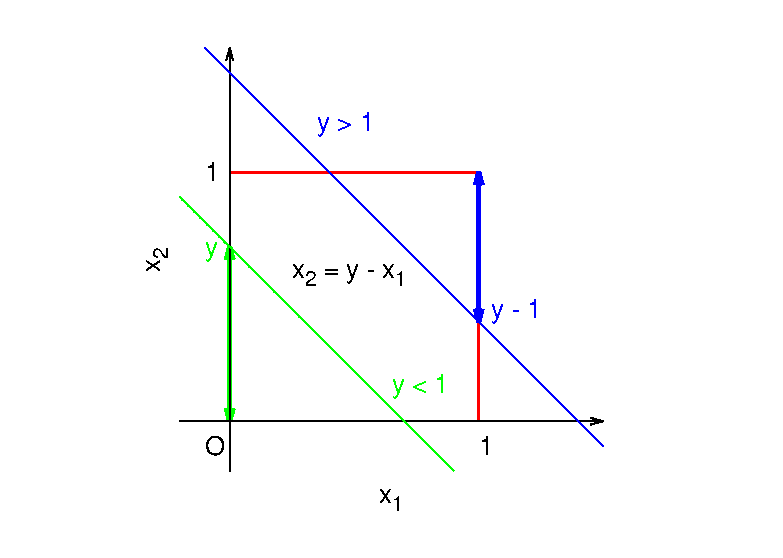
\includegraphics[width=6cm]{./figures/uni_jyouken.eps}
		\caption{$x_1, x_2$ の標本空間と $x_2 = y - x_1$}
		\label{fig:uni_jouken}
\end{figure}



$y = x_1 + x_2$ より $x_2 = y - x_1$ であるので、図 \ref{fig:uni_jouken} に示したように、$0 \leq y \leq 1$ のときに積分範囲は $0 \leq x_2 \leq y$ (図中の緑で示した両矢印の範囲)となり、$1 \leq y \leq 2$ のときは $y − 1 \leq x_2 \leq 1$ と(図中の青の両矢印)なる。

したがって、求める確率密度関数は、

\begin{equation*}
P_Y(y) = 
\begin{cases}
0 \quad (y < 0) \\[8pt]
\displaystyle \int_{0}^{y} 1 \diff x_2 = \left[x_2 \right]_0^y = y \quad (0 \leq y \leq 1) \\[8pt]
\displaystyle \int_{y-1}^{1} 1 \diff x_2 = \left[x_2 \right]_{y-1}^1 = 2-y \quad (1 \leq y \leq 2) \\[8pt]
0 \quad (2 < y)
\end{cases}
\end{equation*}
となる。
\begin{figure}[htb]
	\centering
	    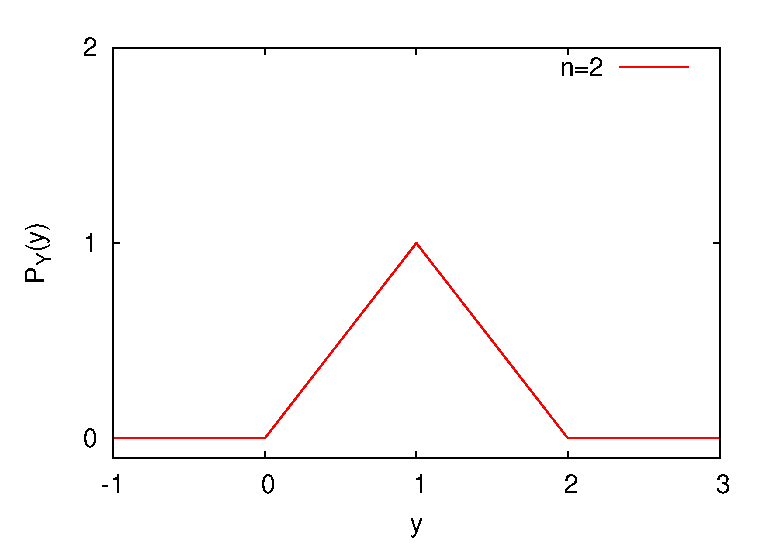
\includegraphics[width=6cm]{./figures/uni_2.eps}
		\caption{二つの一様分布の和の確率密度関数}
		\label{fig:uni_2}
\end{figure}

この結果をプロットすれば以下のように、期待値の和である $y=1$ にピークをとる三角形状となる。

\newpage

\item

上記問題と同様の独立な一様分布に対して、三つの一様分布関数の和である $Y=X_1 + X_2 + X_3$ の確率密度分布を求めよ。

\begin{itembox}[l]{{\bf ヒント:}}

三つの独立な一様分布関数の和 $Y=X_1 + X_2+ X_3$ に対しては、以下を解けばよい。
\begin{equation*}
P_Y(y) = \int_{-\infty}^{\infty} \int_{-\infty}^{\infty} P_1(y - x_1 - x_2) P_2(x_2) P_3 (x_3) \diff x_2 \diff x_3
\end{equation*}

\end{itembox}

{\bf(解答例)}

前問と同様に、$y = x_1 + x_2 + x_3$ とおくと、畳み込み積分の形で以下となる。
\begin{equation*}
P_Y(y) = \int_{-\infty}^{\infty} \int_{-\infty}^{\infty} P_1(y - x_2 - x_3) P_2(x_2) P_3 (x_3) \diff x_2 \diff x_3
\end{equation*}

$y < 0$ あるいは $y>3$ の場合は、必ず $P_Y(y) = 0$ となるので、$0 \leq y \leq 3$ となる範囲において、$x_2, x_3$ の積分範囲を場合わけして考えればよいことになる。

$x_2 = y − x_1 - x_3$ であり、$0 \leq x_1 \leq 1$ だから、
\begin{align*}
y − 1 -x_3 \leq x_ 2 \leq y - x_3
\end{align*}

さらに、$0 \leq x_2 \leq 1$ であるので、以下のように考えることができる。
\begin{align*}
\max (0, y-1-x_3) \leq x_2 \leq \min (1, y-x_3)
\end{align*}

このとき、まず、$x_3$ についての場合わけを行い、
\begin{align*}
(\rm{A})& \quad x_3 \leq y-1 \; \text{のとき、} \; y-1-x_3 \leq x_2 \leq 1 \\[10pt]
(\rm{B})& \quad y-1\leq x_3 \; \text{のとき、} \; 0\leq x_2 \leq y-x_3
\end{align*}



上記の場合わけにおいて、$x_2$ の積分領域が存在するためには、$y − 1 − x_3 \leq 1$、かつ、$0 \leq y − x_3$ となる必要がある。
すなわち、$y − 2 \leq x_ 3 \leq y$ でなければならない。

これと、$0 \leq x_3 \leq 1$ とを比較して、
\begin{align*}
\max(y − 2, 0) \leq x_3 \leq \min(y, 1)
\end{align*}

また、$y \leq 1$ のとき、$(\rm{A})$ を満たす $x_3$ は存在しない。
さらに、$1\leq y − 1$ のときには、$(\rm{B})$ を満たす $x_3$ は存在しない。


これらの場合わけを整理すると、

\begin{description}
\item[$0 \leq y \leq 1$ の場合]
$y-1 \leq x_3$ かつ $0 \leq x_3 \leq y$ であるので、
\begin{align*}
\begin{cases}
0\leq x_3 \leq y \\
0\leq x_2 \leq y-x_3
\end{cases}
\end{align*}

このとき、
\begin{align*}
P_Y(y) 
	&= \int_{0}^{y} \diff x_3 \int_{0}^{y-x_3} \diff x_2 \\
	&= \int_{0}^{y} \diff x_3 (y-x_3) \\
	&= \left[y x_3 - \dfrac{x_3^2}{2} \right]_0^y \\
	&= \dfrac{y^2}{2}
\end{align*}


\item[$1 \leq y \leq 2$ の場合]
$0 \leq x_3 \leq 1$ であるので、
\begin{align*}
\begin{cases}
0\leq x_3 \leq y-1 \\
y-1-x_3\leq x_2 \leq 1
\end{cases}
\end{align*}
あるいは、
\begin{align*}
\begin{cases}
y-1 \leq x_3 \leq 1 \\
0 \leq x_2 \leq y-x_3
\end{cases}
\end{align*}

このとき、
\begin{align*}
P_Y(y) 
	&= \int_{0}^{y-1} \diff x_3 \int_{y-1-x_3}^{1} \diff x_2 + \int_{y-1}^{1} \diff x_3 \int_{0}^{y-x_3} \diff x_2 \\
	&= \int_{0}^{y-1} \diff x_3 [(1 -(y - 1 - x_3)] + \int_{y-1}^{1} \diff x_3 (y - x_3) \\
	&= \left[-y x_3 + \dfrac{x_3^2}{2} +2x_3 \right]_0^{y-1} + \left[y x_3 - \dfrac{x_3^2}{2} \right]_{y-1}^1 \\
	&= \left[ -y (y-1) + \dfrac{(y-1)^2}{2} + 2(y-1) \right] + \left[ \left( y-\dfrac{1}{2} \right) - \left(y (y-1) - \dfrac{(y-1)^2}{2} \right) \right] \\
%	&= -2y^2 + 2y + y^2 -2y + 1 + 2y -2 + y - \dfrac{1}{2} \\
	&= -y^2 + 3y - \dfrac{3}{2}
\end{align*}

\item[$2 \leq y \leq 3$ の場合]
$x_3 \leq y-1$ かつ $y-2 \leq x_3 \leq 1$ であるので、
\begin{align*}
\begin{cases}
y-2 \leq x_3 \leq 1 \\
y-1-x_3\leq x_2 \leq 1
\end{cases}
\end{align*}

このとき、
\begin{align*}
P_Y(y) 
	&= \int_{y-2}^{1} \diff x_3 \int_{y-1-x_3}^{1} \diff x_2 \\
	&= \int_{0}^{y} \diff x_3 [1-(y-1-x_3)] \\
	&= \left[-y x_3 + \dfrac{x_3^2}{2} + 2 x_3 \right]_{y-2}^1 \\
	&= \left[-y + \dfrac{1}{2} +2 -\left(-y (y-2) + \dfrac{(y-2)^2}{2} +2(y-2) \right) \right] \\
%	&= \left[-y + \dfrac{5}{2} +y^2 -2y - \dfrac{(y-2)^2}{2} -2y +4 \right] \\
%	&= \left[\dfrac{13}{2} +y^2 -5y - \dfrac{(y-2)^2}{2}  \right] \\
%	&= \dfrac{1}{2}\left[2y^2 -10y + 13 - y^2 + 4y - 4 \right] \\
	&= \dfrac{1}{2}\left( y^2 -6y + 9 \right) \\
	&= \dfrac{(y-3)^2}{2}
\end{align*}

\end{description}


したがって、求める確率密度関数は、
\begin{equation*}
P_Y(y) = 
\begin{cases}
0 \quad (y < 0) \\[8pt]
\displaystyle 
	\int_{0}^{y} \diff x_3 \int_{0}^{y-x_3} \diff x_2 
	= \dfrac{y^2}{2} \quad (0 \leq y \leq 1) \\[12pt]
\displaystyle 
	\int_{0}^{y-1} \diff x_3 \int_{y-1-x_3}^{1} \diff x_2 + \int_{y-1}^{1} \diff x_3 \int_{0}^{y-x_3} \diff x_2 
	= -y^2 + 3y - \dfrac{3}{2} \quad (1 \leq y \leq 2) \\[12pt]
\displaystyle 
	\int_{y-2}^{1} \diff x_3 \int_{y-1-x_3}^{1} \diff x_2 
	= \dfrac{(y-3)^2}{2} \quad (2 \leq y \leq 3) \\[12pt]
0 \quad (3 < y)
\end{cases}
\end{equation*}
となる。

この結果をプロットすれば以下のように、三角形のグラフから、期待値の和である $y=1.5$ を極大としたベル型のグラフと近づいていることが確認できる。

\begin{figure}[htb]
	\centering
	    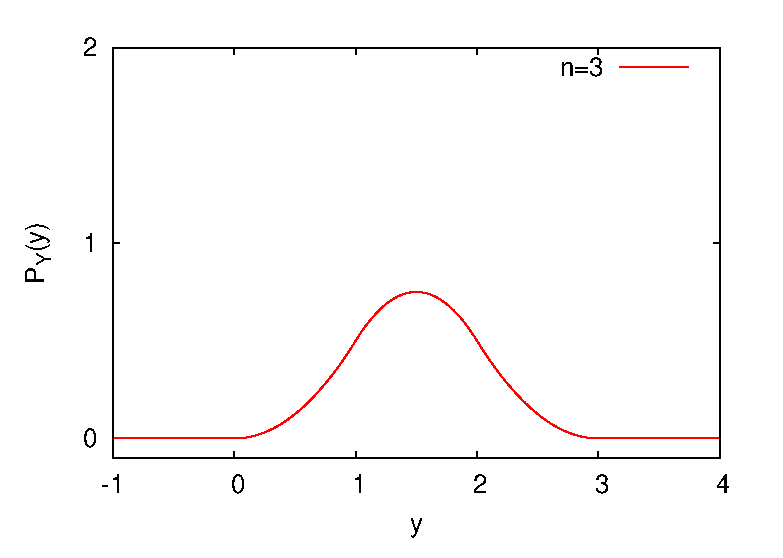
\includegraphics[width=10cm]{./figures/uni_3.eps}
		\caption{三つの一様分布の和の確率密度関数}
		\label{fig:uni_3}
\end{figure}
\color{black}

\newpage
\item

上述の設問において $N$ が十分に大きい場合、コーシー分布のように収束の遅い分布関数を除き、ほとんどの確率分布 $\{ P_i \}$ に対して、中心極限定理が成立する。

平均および分散がそれぞれ、$\bar{X}, \sigma^2$ で表される確率分布 $\{ P_i \}$ に従う $N$ 個の独立な確率変数 $X^{(1)}, X^{(2)}, \cdots, X^{(N)}$ の算術平均 $Y$ を以下のように定めると、$Y$ は新たな確率変数となる。
\begin{equation*}
Y= \dfrac{X^{(1)} + X^{(2)} + \cdots + X^{(N)} }{N}
\end{equation*}

この時の確率変数 $Y$ の分布関数が以下のガウス分布となることを示せ。
\begin{equation*}
P_Y(y) = \dfrac{1}{\sqrt{2 \pi \sigma^2/N}} \exp \left(-\dfrac{(y-\bar{X})^2}{2 \sigma^2/N} \right)
\end{equation*}

\begin{itembox}[l]{{\bf ヒント:}}

まず、$Y$ の期待値および分散の「定数倍」と「和」の性質を利用して、期待値および分散を求め、これをガウス分布の期待値と分散であるとみなせばよい。

\end{itembox}

{\bf (解答例)}

$Y$ の期待値 $E(Y)$ は以下のように展開できる。
\begin{align*}
E(Y)
	&= E \left(\dfrac{X^{(1)} + X^{(2)} + \cdots + X^{(N)} }{N} \right) \\
	&= \dfrac{1}{N} E \left(X^{(1)} + X^{(2)} + \cdots + X^{(N)} \right) \\
	&= \dfrac{1}{N} \left\{ E (X^{(1)}) + E(X^{(2)}) + \cdots + E(X^{(N)}) \right\} \\
	&= \dfrac{1}{N} \times N \times \bar{X} \\
	&= \bar{X}
\end{align*}
なお、二行目へは「期待値の定数倍」の性質を、また、三行目へは「確率変数の期待値の和」の性質をそれぞれ利用した。

一方、確率変数 $X^{(1)}, X^{(2)}, \cdots, X^{(N)}$ が独立であることから、$Y$ の分散 $V(Y)$ は以下のように展開できる。
\begin{align*}
V(Y)
	&= V \left(\dfrac{X^{(1)} + X^{(2)} + \cdots + X^{(N)} }{N} \right) \\
	&= \left(\dfrac{1}{N} \right)^2 V \left(X^{(1)} + X^{(2)} + \cdots + X^{(N)} \right) \\
	&= \dfrac{1}{N^2} \left\{ V (X^{(1)}) + V(X^{(2)}) + \cdots + V(X^{(N)}) \right\} \\
	&= \dfrac{1}{N^2} \times N \times \sigma^2 \\
	&= \dfrac{1}{N} \sigma^2
\end{align*}
なお、二行目へは「分散の定数倍」の性質を利用した。
また、三行目へは「それぞれの確率変数が独立である」から、「分散の和」の性質を利用できた。



これらの結果から、期待値は元の確率変数と同様なものとなるが、分散はサンプリング数の増加に伴い、$1/\sqrt{N}$ で小さくなっていくことが理解できる。
%このことから、巨視的な気体の振る舞いが

\color{black}

このとき、上記の期待値および分散を用いて、求める確率変数 $Y$ の分布関数は以下のガウス分布で表すことができる。
\begin{equation*}
P_Y(y) = \dfrac{1}{\sqrt{2 \pi \sigma^2/N}} \exp \left(-\dfrac{(y-\bar{X})^2}{2 \sigma^2/N} \right)
\end{equation*}


\color{black}

\end{enumerate}

\newpage


%\subsection{物理数学}
%
%\subsubsection{フーリエ変換}
%
%\newpage

\color{black}

\subsection{熱力学}


\subsubsection{熱力学ポテンシャルの一般的性質}

\begin{boxnote}
系に課せられた各種の拘束条件と、それに対応する統計集団(アンサンブル)および熱力学ポテンシャル(自由エネルギー)との関係を確認する問題です。

種々の熱力学的な拘束条件(温度が一定とか圧力が一定など)の下での平衡状態を求める場合に、熱力学ポテンシャルは非常に有効な手段である。
それは、与えられた拘束条件の下で、対応する熱力学ポテンシャルが最小になるため、平衡状態を求める問題は、熱力学ポテンシャルの最小化問題に帰着できるからである。


\end{boxnote}

\vspace{10pt}

\begin{enumerate}
\setlength{\parskip}{0cm} % 段落間
\setlength{\itemsep}{0.5cm} % 項目間
\item
体積 $V$、粒子数 $N$、内部エネルギー $E$ が一定の系(孤立系)の平衡状態で極値を取る熱力学量を示せ。

%\vspace{10pt}
\begin{itembox}[l]{{\bf ヒント:}}
この例の場合のみ、最小化問題ではなく最大化問題になる。
\end{itembox}


\item
上の結果を用いて、以下の各変数が一定の系の平衡状態を記述するのに適した自由エネルギーを求めよ。
%\vspace{10pt}

\begin{itembox}[l]{{\bf ヒント:}}
上記の設問の解答から、ルジャンドル変換により、独立な変数を変換すれば導出できる。
\end{itembox}

\begin{enumerate}
\item
体積 $V$、粒子数 $N$、温度 $T$ が一定の系(カノニカル系)

\item
体積 $V$、化学ポテンシャル $\mu$、温度 $T$ が一定の系(グランドカノニカル系)
\item
圧力 $P$、粒子数 $N$ 、温度 $T$ が一定の系(T-p分布と呼ばれる)

\end{enumerate}

\end{enumerate}

\newpage







\begin{enumerate}
\setlength{\parskip}{0cm} % 段落間
\setlength{\itemsep}{0.5cm} % 項目間
\item
体積 $V$、粒子数 $N$、内部エネルギー $E$ が一定の系(孤立系)の平衡状態で極値を取る熱力学量を示せ。

\begin{itembox}[l]{{\bf ヒント:}}
この例の場合のみ、最小化問題ではなく最大化問題になる。
\end{itembox}

\vspace{10pt}

{\bf (解答例)}

熱力学の第二法則より、孤立系において、不可逆過程により系が変化した場合、常にエントロピーが増加するのであった(エントロピー増大則)。

系の平衡状態とは、系中において物質やエネルギー(熱)の正味の流れがなく、系が変化しなくなった状態と考えることができる。
上記の増大則にしたがって系のエントロピーは増加し続けてきたのであるから、この平衡状態において系のエントロピーは最大化すると考えることができる。

したがって、孤立系の平衡状態を表す熱力学量はエントロピーであり、平衡状態において最大化する。

これを、微分表現で表せば、
\begin{equation*}
\diff S \geq \dfrac{\diff E}{T} + \dfrac{P \diff V}{T} + \dfrac{\sum_i \mu_i \diff N_i}{T}
\end{equation*}
となる。

このとき、独立変数である体積 $V$、粒子数 $N$、内部エネルギー $E$ を一定、すなわち、右辺が 0 となる場合に $S \geq 0$ となり、エントロピーが最大化し、等号成立は平衡状態の場合のみとなる。



\newpage

\item
上の結果を用いて、以下の各変数が一定の系の平衡状態を記述するのに適した自由エネルギーを求めよ。

\begin{itembox}[l]{{\bf ヒント:}}
上記の設問の解答から、ルジャンドル変換により、独立な変数を変換すれば導出できる。
\end{itembox}

\vspace{10pt}

\begin{enumerate}
\item
体積 $V$、粒子数 $N$、温度 $T$ が一定の系(カノニカル系)


\vspace{10pt}
{\bf (解答例)}

内部エネルギーの式は、内部エネルギー $E$ の微小変化 $dE$ を、エントロピー $S$、体積 $V$、および、粒子数 $N$ の微小変化である $\diff S, \diff V, \diff N$ により、
\begin{equation*}
\diff E \leq T \diff S - P \diff V + \mu \diff N
\end{equation*}

これを、$S, V, N$ を独立な変数とする内部エネルギーの関数であると見て、$E(S, V, N)$と書くことにする。
求めるカノニカル系での自由エネルギーは、$T, V, N$ を独立な変数とする関数として $F(T, V, N)$ と書くことができる。
したがって、$E(S, V, N) \Rightarrow F(T, V, N)$ という変数変換を行う必要がある。

積の微分公式から、
\begin{align*}
\diff (TS) = S \diff T + T \diff S \notag \\
\therefore T \diff S = \diff (TS) - S \diff T
\end{align*}
	 	
これを、内部エネルギーの式に代入し、更に変形すると、
\begin{align*}
\diff E \leq \diff (TS) - S \diff T - P \diff V + \mu \diff N \notag \\
\diff (E-TS) \leq -S \diff T - P \diff V + \mu \diff N
\end{align*}

ここで、求めるカノニカル系の自由エネルギーを $F(T,V,N) = E-TS$ として、
\begin{equation*}
\diff F(T,V,N) \leq -S \diff T - P \diff V + \mu \diff N
\end{equation*}
	 	
これで、温度 $T$、体積 $V$、および、粒子数 $N$ を独立変数とするカノニカル系の自由エネルギー(ヘルムホルツエネルギー)の表式が求まった。

なお、独立変数である体積 $V$、粒子数 $N$、温度 $T$ が一定となった場合に右辺が 0 となり、$\diff F \leq 0$ で最小化し、平衡状態で等号が成立する。

\color{black}

\vspace{10pt}
\item
体積 $V$、化学ポテンシャル $\mu$、温度 $T$ が一定の系(グランドカノニカル系)



\vspace{10pt}
{\bf (解答例)}

求めるグランドカノニカル系での自由エネルギーを、$\Omega(T, V, \mu)$ とすると、$F(T, V, N) \Rightarrow J(T, V, \mu)$ という変数変換を行えばよいことになる。

積の微分公式から、
\begin{align*}
\diff (N \mu) = N \diff \mu + \mu \diff N \notag \\
\therefore \mu \diff N = \diff (N \mu) - N \diff \mu
\end{align*}
	 	
これを、前述のヘルムホルツエネルギーの式に代入し、更に変形すると、
\begin{align*}
\diff F \leq -S \diff T - P \diff V + N \mu - N \diff \mu \notag \\
\diff \left(F - N \mu \right) \leq -S \diff T - P \diff V - N \diff \mu
\end{align*}

ここで、求めたいグランドカノニカル系の自由エネルギーを $\Omega(T,V,\mu) = F - N \mu$ として、
\begin{equation*}
\diff \Omega(T,V,\mu) \leq -S \diff T - P \diff V - N \diff \mu
\end{equation*}
	 	
これで、温度 $T$、体積 $V$、および、化学ポテンシャル $\mu$ を独立変数とするグランドカノニカル系での自由エネルギー(グランドポテンシャルと呼ばれる) $\Omega$ の表式が求まる。
これは、独立変数が一定となる条件で、$\Omega \leq 0$ となり、平衡状態で最小化する。

\color{black}
\vspace{10pt}
\item
圧力 $P$、粒子数 $N$ 、温度 $T$ が一定の系(T-p分布と呼ばれる)



\vspace{10pt}
{\bf (解答例)}

指定された系での自由エネルギーを、$G(T, P, N)$ とすると、ヘルムホルツエネルギー $F$ から、$F(T, V, N) \Rightarrow J(T, P, N)$ という変数変換を行う必要がある。

積の微分公式から、
\begin{align*}
\diff (PV) = P \diff V + V \diff P \notag \\
\therefore  P \diff V = \diff (PV) - V \diff P
\end{align*}
	 	
これを、ヘルムホルツエネルギーの式に代入し、更に変形すると、
\begin{align*}
\diff F &\leq -S \diff T - [\diff (PV) -V \diff P] + \mu \diff N \notag \\
\diff (F + PV) &\leq -S \diff T + V \diff P + \mu \diff N
\end{align*}

ここで、求める自由エネルギーを $G(T,P,N) = F + PV$ として、
\begin{equation*}
\diff G(T,P,N) \leq -S \diff T + V \diff P + \mu \diff N
\end{equation*}
	 	
これで、温度 $T$、圧力 $P$、および、粒子数 $N$ を独立変数とする指定された系での自由エネルギー(ギッブスエネルギー) $G$ の表式が求まる。
なお、独立変数を一定とすれば、$\diff G \leq 0$ となる。
等号成立は、平衡状態の時である。

\end{enumerate}

\newpage


\end{enumerate}

\color{black}


\newpage



\newpage

%**********************************************************************
%                              問2
%**********************************************************************

\subsubsection{理想気体の断熱自由膨張}
\label{sec:dan_netsu_jiyuu}


\begin{boxnote}
{\bf 出題意図:}
理想気体の断熱自由膨張がエントロピーが増加する不可逆過程であることを、熱力学の観点から確認する問題です。
後程、「\ref{sec:dan_netsu_toukei} 理想気体の断熱自由膨張の2」において、統計力学的な観点からの検討も行います。
\end{boxnote}

\color{black}

\vspace{8pt}

断熱固体壁で囲まれた体積 $V$ の容器の中央を仕切り、それぞれ体積 $V/2$ の2つの領域 A と B に分ける。
領域 A を温度 $T$ の1モルの理想気体で満たし、一方領域 B は真空にした状態で平衡に保つとする。
この状態から仕切りを取り除くと、領域 A の気体は領域 B の方へと拡散し、やがて気体は領域 A と領域 B を等しく満たした状態で新たな平衡に達した。

この理想気体の断熱自由膨張に関して、以下の問いに答えよ。

\begin{enumerate}
\setlength{\parskip}{0cm} % 段落間
\setlength{\itemsep}{0.3cm} % 項目間

\item
粒子数一定の系の Helmholtz の自由エネルギー $F$ を、温度 $T$ と体積 $V$ の関数として $F(T,V)$ と表すとき、その全微分 $dF$ を共役な変数 $S,P$ を用いて表せ。


\begin{itembox}[l]{{\bf ヒント:}}

内部エネルギー $E$ の微分表現からルジャンドル変換すればよい。

\end{itembox}

\color{black}

\item
前問で導出した全微分形式を用いて、以下の Maxwell の関係式を証明せよ。
\begin{equation*}
\Bigl( \frac{\partial S}{\partial V} \Bigr)_T = \Bigl( \frac{\partial P}{\partial T} \Bigr)_V
\end{equation*}


\begin{itembox}[l]{{\bf ヒント:}}

Helmholtz の自由エネルギー $F$ の全微分形式での表記である以下を前問の結果と比較すればよい。
\begin{align*}
dF = \left( \dfrac{\partial F}{\partial T} \right)_V dT + \left( \dfrac{\partial  F}{\partial V} \right)_T dV
\end{align*}

\end{itembox}

\color{black}

\item
1 モルの理想気体の状態方程式 $PV = RT$ を用いて $(\partial E / \partial V)_T$ を計算することにより、理想気体の内部エネルギー $E$ が温度 $T$ だけの関数であることを示せ。


\begin{itembox}[l]{{\bf ヒント:}}

内部エネルギーの体積依存を表す $\left(\dfrac{\partial E}{\partial V} \right)_T$ が 0 となることを示せばよい。

\end{itembox}

\color{black}

\item
\label{part: ref1}
最初の平衡状態(始状態: initial)と最後の平衡状態(終状態: final)における全系のエントロピーの値を $S_{i}$ および $S_{f}$ とするとき、エントロピー変化量
\begin{equation*}
\Delta S = S_{i} - S_{f} = \int_{\rm initial}^{\rm final} dS
\end{equation*}
を{\bf 「熱力学的に計算」}することにより、上記の現象が不可逆過程であることを示せ。

\begin{itembox}[l]{{\bf ヒント:}}

エントロピーは状態量であることを利用するとよい。

具体的には、任意の適正な準静的過程を経由して比較したい二つの状態変化を再現してやれば、状態量としての結果は常に等しいので、単純に差を取ればよいことになる。

\end{itembox}
\color{black}

\end{enumerate}

\newpage


\begin{enumerate}
\setlength{\parskip}{0cm} % 段落間
\setlength{\itemsep}{0.3cm} % 項目間

\item
粒子数一定の系の Helmholtz の自由エネルギー $F$ を、温度 $T$ と体積 $V$ の関数として $F(T,V)$ と表すとき、その全微分 $dF$ を共役な変数 $S,P$ を用いて表せ。
\vspace{8pt}

\begin{itembox}[l]{{\bf ヒント:}}

内部エネルギー $E$ の微分表現からルジャンドル変換すればよい。

\end{itembox}

{\bf (解答例)}

Helmholtz の自由エネルギー $F$ は、温度 $T$ と体積 $V$、および、粒子数 $N$ を自然な変数の組とし、それらの変数が与えられたときに、系の平衡状態における熱力学的性質の情報をすべて持つ完全な熱力学関数となるのであった
\footnote
{
ここでの、「熱力学的性質の情報をすべて持つ」ということの意味は、この関数を対応する変数で偏微分することにより、その変数に共役な状態量をすべて導出できるという意味である。

なお、共役な変数(状態量)とは、例えば、内部エネルギー $E(S, V, N)$ を例にとれば、以下のように対応する $S \leftrightarrow T, V \leftrightarrow P, N_i \leftrightarrow \mu_i$ のような示量性変数と示強性変数の組み合わせのことを指している。
\begin{align*}
\begin{cases}
T(S, V, N) = \left(\difp{E(S, V, N)}{S} \right)_{V, N} \\[10pt]
P(S, V, N) = - \left(\difp{E(S, V, N)}{V} \right)_{S, N} \\[10pt]
\mu_i(S, V, N) = \left(\difp{E(S, V, N)}{N_i} \right)_{S, V} \\
\end{cases}
\end{align*}

}。

設問に示された系では、粒子数一定で、温度 $T$ と体積 $V$ の関数として $F(T,V)$ と表すのであるから完全な熱力学関数となり、その全微分は自然な変数の微分 $\diff T, \diff V$ と共役な変数 $S, P$ との積の形で書けることになる。

具体的な表式としては、示量変数 $S, V$ を自然な変数の組とする内部エネルギー $E$ の全微分表現 $\diff E = T \diff S - P \diff V$ からのルジャンドル変換により、示量変数であるエントロピー $S$ を示強変数である温度 $T$ に変換することで導出することができる。
\begin{align*}
\diff F 
	&= \diff(E-TS) \\
	&= (T \diff S - P \diff V) -(\diff T S + T \diff S) \\
	&=-S \diff T -P \diff V
\end{align*}

\color{black}

\newpage

\item
前問で導出した全微分形式を用いて、以下の Maxwell の関係式を証明せよ。
\begin{equation*}
\Bigl( \frac{\partial S}{\partial V} \Bigr)_T = \Bigl( \frac{\partial P}{\partial T} \Bigr)_V
\end{equation*}


\begin{itembox}[l]{{\bf ヒント:}}

Helmholtz の自由エネルギー $F$ の全微分形式での表記である以下を前問の結果と比較すればよい。
\begin{align*}
dF = \left( \dfrac{\partial F}{\partial T} \right)_V dT + \left( \dfrac{\partial  F}{\partial V} \right)_T dV
\end{align*}

\end{itembox}

{\bf (解答例
\footnote{
Maxwell の関係式に関する参考事項:\href{http://kisokouza.island.ac/documents/Thermo_Dynamics_basics.pdf}{「熱力学の基礎的事項」の「5.1 マクスウェルの関係式」}
}
)}

Helmholtz の自由エネルギー $F$ は、全微分で以下のように書くこともできる。
\begin{align*}
dF = \left( \dfrac{\partial F}{\partial T} \right)_V dT + \left( \dfrac{\partial  F}{\partial V} \right)_T dV
\end{align*}

独立変数は線形独立なので 上式を、前問の解の係数と比較して、
\begin{align*}
\begin{cases}
\left( \dfrac{\partial F}{\partial T} \right)_V = -S \\[10pt]
\left( \dfrac{\partial  F}{\partial V} \right)_T = -P
\end{cases}
\end{align*}
を得る。

このとき、
\begin{align*}
\left( \dfrac{\partial S}{\partial V} \right)_T 
	&= \dfrac{\partial}{\partial V} \left[ \left( - \dfrac{\partial F}{\partial T} \right)_V \right]_T \\
	&= \left( - \dfrac{\partial^2 F}{\partial T \partial V} \right)_{V, T} \\
	&= \left( \dfrac{\partial P}{\partial T} \right)_{V} 
\end{align*}
なお、二行目への変換で二階微分の連続性を利用している。
\newpage

\item
1 モルの理想気体の状態方程式 $PV = RT$ を用いて $(\partial E / \partial V)_T$ を計算することにより、理想気体の内部エネルギー $E$ が温度 $T$ だけの関数であることを示せ。
\vspace{8pt}

\begin{itembox}[l]{{\bf ヒント:}}

内部エネルギーの体積依存を表す $\left(\dfrac{\partial E}{\partial V} \right)_T$ が 0 となることを示せばよい。

\end{itembox}
\vspace{8pt}

{\bf (解答例)}

粒子数 $N$ が一定、すなわち、$\diff N = 0$ のとき、内部エネルギーの全微分 $\diff E$ は、以下のように書くことができる。
\begin{equation*}
\diff E = T \diff S - P \diff V
\end{equation*}

上式の両辺を $\diff V$ で割って、温度一定の条件のもとで $\diff V \rightarrow 0$ とすると、
\begin{align*}
\left(\dfrac{\partial E}{\partial V} \right)_T 
	&= T \left(\dfrac{\partial S}{\partial V} \right)_T -P \\
	&= T \left(\dfrac{\partial P}{\partial T} \right)_V -P \\
	&= T \left(\dfrac{\partial}{\partial T} \dfrac {RT}{V} \right)_V -P \\
	&= T \left(\dfrac {R}{V}\right) -P \\
	&= 0
\end{align*}

なお、二行目への展開では、前問でのマックスウェルの関係式である、$\left(\dfrac{\partial S}{\partial V} \right)_T = \left(\dfrac{\partial P}{\partial T} \right)_V$ を用い、三行目と四行目では、理想気体の状態方程式から、$P = \dfrac {RT}{V}$ を利用した。

上式に示したように、内部エネルギーの体積依存を表す $\left(\dfrac{\partial E}{\partial V} \right)_T = 0$ であるから、内部エネルギーは体積に依存しないことになる。
したがって、理想気体の内部エネルギー $E$ は温度 $T$ だけの関数となる。

\newpage

\item
\label{part: ref1}
最初の平衡状態(始状態: initial)と最後の平衡状態(終状態: final)における全系のエントロピーの値を $S_{i}$ および $S_{f}$ とするとき、エントロピー変化量
\begin{equation}
\Delta S = S_{i} - S_{f} = \int_{\rm initial}^{\rm final} dS
\end{equation}
を{\bf 「熱力学的に計算」}することにより、上記の現象が不可逆過程であることを示せ。
\vspace{8pt}

\begin{itembox}[l]{{\bf ヒント:}}

エントロピーは状態量であることを利用するとよい。

具体的には、任意の適正な準静的過程を経由して比較したい二つの状態変化を再現してやれば、状態量としての結果は常に等しいので、単純に差を取ればよいことになる。

\end{itembox}

{\bf (解答例)}

断熱自由膨張は、断熱であることから系外との熱のやり取りは生じないので、$\Delta Q = 0$ である。
また、自由膨張であるから系外に仕事をするわけではないので、$\Delta W = 0$ となる。
したがって、内部エネルギー変化 $\Delta E = 0$ となる。
ここで対象としているのは理想気体であるから、温度変化も生じないことになる。

エントロピーは平衡状態に対してのみ定義されるため、準静的な変化以外では経路に沿ったエントロピー変化は計算できない。
同時に、「エントロピーは状態量である」から、経路に関わらず、二つの状態の差を見れば変化量が議論できることになる。

つまり、エントロピー変化量を算出するためには、任意の適正な準静的過程を経由して、比較したい二つの状態変化を再現し、単純にそれらの差を取ればよいことになる。

ここでは、等温可逆過程で考えることにしよう。

このとき、気体がする仕事は、
\begin{equation*}
\Delta W = -\int PdV = -\int (RT/V) dV = -RT \ln \left(\dfrac{2V}{V} \right) = -RT \ln 2
\end{equation*}
となる。

等温過程で内部エネルギーは変化していないのだから、$\Delta E = \Delta Q+ \Delta W =0$ より、$\Delta Q=-\Delta W$ であり、結局、$\Delta Q = RT \ln 2$ となる。

従ってこの気体のエントロピー変化は
\begin{equation*}
\Delta S= \dfrac{\Delta Q}{T} = R \ln 2
\end{equation*}
となる。

孤立系においてエントロピーが増大していることより、この断熱膨張という現象は、不可逆過程である。

\color{black}

\end{enumerate}

\newpage


\section{統計物理}

\subsection{エントロピーについて}


\subsubsection[統計力学エントロピー]{統計力学エントロピー \protect \footnote{出典:「Kardar: Statistical Physics of Particles, Capter 3 章末問題2」を参考にし、改変。}}

%**********************************************************************
%       問1(Kardar: Statistical Physics of Particles, Capter 3 章末問題2)
%**********************************************************************

\begin{boxnote}
{\bf 出題意図:}
エントロピーの微視的な定義を確認します。
そのうえで、孤立系における位相空間中での代表点の運動(等エネルギー面上での運動)が可逆な過程になっていて、エントロピーの増加をもたらさないことを確認する問題です。
\end{boxnote}

\vspace{8pt}


\begin{enumerate}
\setlength{\parskip}{0cm} % 段落間
\setlength{\itemsep}{0.3cm} % 項目間

\item
ある孤立系の $j$ 番目の微視的状態が実現する確率を $P_j$ と書き、その集合である $\{ P_j \}$ を用いて{\bf 統計力学}エントロピーを下式によって定義する
\footnote{
統計力学エントロピーのこの表式の導出:\href{http://kisokouza.island.ac/documents/Stat_Phys_Entropy.pdf}{「統計力学エントロピー」の「3.3 具体的な計算」}
}。
\begin{equation*}
  S = -k_{\rm B} \sum_j P_j \ln P_j
  \label{eq: SM_S}
\end{equation*}

孤立系で上記の統計力学エントロピーを最大化することが、孤立系の平衡状態ではすべての微視状態が等確率で現れるという「等重率の原理」と矛盾しない結果を導くことを示せ。


\begin{itembox}[l]{{\bf ヒント:}}

ミクロカノニカル集団%(粒子数 $N$、体積 $V$、内部エネルギー $E$ が一定)
の拘束条件である「各微視的状態の出現確率 $P_j$ の合計は $1$ に等しい 」を用いて、ラグランジュの未定乗数により最大化問題を解けばよい。

\end{itembox}

\color{black}

\item
上述の統計力学エントロピーが時間変化しないことを示せ。

\begin{itembox}[l]{{\bf ヒント:}}
系を記述するハミルトニアンを $\mathcal{H}$ とすると、位相空間 $\Gamma \equiv ( \{ q_{\mu}(t) \},~ \{ p_{\mu}(t) \} )$ での代表点の密度分布 $\rho(\Gamma,t)$ の時間発展は、以下のリウビル方程式に従う
\footnote
{
リウビル方程式については:\href{http://kisokouza.island.ac/documents/Stat_Phys_Entropy.pdf}{「位相空間の直観的な理解」} を参照されたい。
}。
\begin{equation*}
\frac{\partial \rho}{\partial t} 
+ \sum_{\mu = 1}^{f} 
\left[
\difp{\rho}{q_{\mu}}
\difp{\mathcal{H}}{p_{\mu}}
- \difp{\rho}{p_{\mu}}
\difp{\mathcal{H}}{q_{\mu}}
\right]
= 0
\end{equation*}

このリウビルの方程式の分布関数 $\rho(\Gamma, t)$ を、上述の式中の $\{ P_j \}$ と同一視($\rho$ と $P_j$ の規格化定数などの定数分の差は無視)して以下のように定義し、$\difd{S(t)}{t} = 0$ を示せばよい。
\begin{equation*}
	S(t) = - \int \diff \Gamma \rho(\Gamma,t) \ln \rho(\Gamma, t)
\end{equation*}

\end{itembox}

\color{black}

\end{enumerate}

\newpage

%ある孤立系の $j$ 番目の微視的状態が実現する確率を $P_j$ と書き、$\{ P_j \}$ を用いて{\bf 統計力学}エントロピーを下式によって定義する
%\footnote{
%統計力学エントロピーのこの表式の導出:\href{http://kisokouza.island.ac/documents/Stat_Phys_Entropy.pdf}{「統計力学エントロピー」の「3.3 具体的な計算」}
%}。
%この統計力学エントロピーに関する以下の設問に答えよ。
%\begin{equation*}
%  S = -k_{\rm B} \sum_j P_j \ln P_j
%  \label{eq: SM_S}
%\end{equation*}



\vspace{8pt}

\begin{enumerate}
\setlength{\parskip}{0cm} % 段落間
\setlength{\itemsep}{0.3cm} % 項目間
%
%\item
%孤立系に対して{\bf 熱力学}エントロピーが満たすべき基本的な条件を述べよ。


\item
ある孤立系の $j$ 番目の微視的状態が実現する確率を $P_j$ と書き、その集合である $\{ P_j \}$ を用いて{\bf 統計力学}エントロピーを下式によって定義する
\footnote{
統計力学エントロピーのこの表式の導出:\href{http://kisokouza.island.ac/documents/Stat_Phys_Entropy.pdf}{「統計力学エントロピー」の「3.3 具体的な計算」}
}。
\begin{equation*}
  S = -k_{\rm B} \sum_j P_j \ln P_j
  \label{eq: SM_S}
\end{equation*}

孤立系で上記の統計力学エントロピーを最大化することが、孤立系の平衡状態ではすべての微視状態が等確率で現れるという「等重率の原理」と矛盾しない結果を導くことを示せ。

\begin{itembox}[l]{{\bf ヒント:}}

ミクロカノニカル集団%(粒子数 $N$、体積 $V$、内部エネルギー $E$ が一定)
の拘束条件である「各微視的状態の出現確率 $P_j$ の合計は $1$ に等しい 」を用いて、ラグランジュの未定乗数により最大化問題を解けばよい。

\end{itembox}

{\bf (解答例)}

孤立系であるので、ミクロカノニカル集団(粒子数 $N$、体積 $V$、内部エネルギー $E$ が一定)を対象として考えることになる
\footnote{
ミクロカノニカル集団に関する参考事項:\href{http://kisokouza.island.ac/documents/Stat_Phys_Entropy.pdf}{「統計力学エントロピー」の「4.3 ミクロカノニカル集団」}
}。

この場合の拘束条件とは、「各微視的状態の出現確率 $P_j$ の合計は $1$ に等しい 」となる。
\begin{equation*}
\sum_j P_j = 1
\end{equation*}

このとき、上記の拘束条件を用いて、ラグランジュの未定乗数により以下の最大化問題を解く。
\begin{equation*}
\max_{\{ P_j \}} \left[ -k_B \sum_k P_k \ln P_k + \lambda \left( \sum_k P_k - 1 \right) \right]
\end{equation*}

未定定数を導入したため、各 $P_j$ は独立変数とみなしてもよいので、最大化の条件は、
\begin{equation*}
\frac{\partial}{\partial P_j} \left[ -k_B \sum_k P_k \ln P_k + \lambda \left( \sum_k P_k - 1 \right) \right] = 0
\end{equation*}
という関係式を各 $P_j$ について解けばよいことになる。

これらから、次の解が得られる。
\begin{align*}
&-k_B (\ln P_k + 1) + \lambda = 0 \notag \\
\therefore &\quad P_j = \exp \left(\frac{\lambda}{k_B} -1 \right)
\end{align*}

上式の右辺は $j$ に依存していなくて、変数 $\lambda$ はすべての式において同一であるから、結局、すべての $P_j$ が等しいことになる。

このことは、{\bf 「ミクロカノニカル集団では、等エネルギー面上の可能な微視的状態はすべて同じ確率で実現する」という「等重率の原理」}を表している。

\newpage

\item
上述の統計力学エントロピーが時間変化しないことを示せ。


\begin{itembox}[l]{{\bf ヒント:}}
系を記述するハミルトニアンを $\mathcal{H}$ とすると、位相空間 $\Gamma \equiv ( \{ q_{\mu}(t) \},~ \{ p_{\mu}(t) \} )$ での代表点の密度分布 $\rho(\Gamma,t)$ の時間発展は、以下のリウビル方程式に従う
\footnote
{
リウビル方程式については:\href{http://kisokouza.island.ac/documents/Stat_Phys_Entropy.pdf}{「位相空間の直観的な理解」} を参照されたい。
}。
\begin{equation*}
\difd{\rho}{t} 
=
\difp{\rho}{t} 
+ \sum_{\mu = 1}^{f} 
	\left[
		\difp{\rho}{q_{\mu}}\dot{q}_{\mu}
		- \difp{\rho}{p_{\mu}}\dot{q}_{\mu}
	\right]
= 0
\end{equation*}

このリウビルの方程式の分布関数 $\rho(\Gamma, t)$ を、上述の式中の $\{ P_j \}$ と同一視($\rho$ と $P_j$ の規格化定数などの定数分の差は無視)して以下のように定義し、$\difd{S(t)}{t} = 0$ を示せばよい。
\begin{equation*}
	S(t) = - \int \diff \Gamma \rho(\Gamma,t) \ln \rho(\Gamma, t)
\end{equation*}

\end{itembox}

\vspace{8pt}

{\bf (解答例)}

代表点の密度分布 $\rho(\Gamma,t)$ の分布関数を、微視的状態の出現確率 $P_j$ と同一視すれば、時間の関数としてのエントロピー $S(t)$ は
\begin{equation*}
	S(t) = - \int \diff \Gamma \rho(\Gamma,t) \ln \rho(\Gamma, t)
\end{equation*}
と書くことができる。
なお、規格化定数などの定数分の差は無視した。

上記のエントロピー $S(t)$ の時間変化が $0$、すなわち、 $dS(t)/dt = 0$ を示せばよいわけである。
\begin{align*}
\dfrac{d S(t)}{dt} 
	&= - \difd{}{t} \int \diff \Gamma \rho(\Gamma,t) \ln \rho(\Gamma, t) \\
	&= - \int \diff \Gamma 
		\left\{ 
			\difp{\rho(\Gamma,t)}{\rho} \difd{\rho}{t} \ln \rho 
			+ \rho \difp{\ln \rho(\Gamma,t)}{\rho} \difd{\rho}{t} 
		\right\} \\
	&= - \int \diff \Gamma \big( \ln \rho + 1 \big)\difd{\rho}{t} \\
	&= 0
\end{align*}

なお、最後の行へは、リウビルの定理から以下の関係があることを用いている
\footnote{
リウビルの定理に関する参考事項:\href{http://kisokouza.island.ac/documents/Phase_Space.pdf}{「位相空間の直観的な理解」}の「3 リウビルの定理」を参照されたい。
}。
\begin{align*}
\difd{\rho}{t} 
=
\difp{\rho}{t} 
+ \sum_{\mu = 1}^{f} 
	\left[
		\difp{\rho}{q_{\mu}}\dot{q}_{\mu}
		- \difp{\rho}{p_{\mu}}\dot{q}_{\mu}
	\right]
= 0
\end{align*}

ここで導かれた関係は、\textbf{「我々が系を構成する 1 個 1 個の粒子の状態($\Gamma$ 空間)を指定できるくらいに詳細な情報を持っている場合には、エントロピーは変化しない」} と言うことを表現していることになり、\textbf{「エントロピー増大則が、系を粗視化して見たときに出現する性質、すなわち、我々が完全なミクロな情報にアクセスできないことによる情報の欠落に起因するものであること」} を意味している。 
\color{black}

\end{enumerate}



\newpage

%**********************************************************************
%                              問2
%**********************************************************************
\subsubsection{理想気体の断熱自由膨張(2)}
\label{sec:dan_netsu_toukei}

\begin{boxnote}
{\bf 出題意図:}
理想気体の断熱自由膨張について、熱力学の項で、「\ref{sec:dan_netsu_jiyuu} 理想気体の断熱自由膨張」として取り扱った演習問題と同様なものを、統計力学の観点から再確認する問題です。
\end{boxnote}
\vspace{8pt}

断熱固体壁で囲まれた体積 $V$ の容器の中央を仕切り、それぞれ体積 $V/2$ の2つの領域 A と B に分ける。
領域 A を温度 $T$ の1モルの理想気体で満たし、一方領域 B は真空にした状態で平衡に保つとする。
この状態から仕切りを取り除くと、領域 A の気体は領域 B の方へと拡散し、やがて気体は領域 A と領域 B を等しく満たした状態で新たな平衡に達した。


理想気体を $N$ 個の互いに相互作用しない粒子の集団であると見なし ($N \gg 1$ とする)、設問 (d) で計算したエントロピー変化をミクロカノニカル集団の方法により {\bf 「統計力学的」に導出せよ}。

ただし、問題を簡単にするために、各粒子の微視的状態としては、粒子の位置座標だけを考慮するものとし、運動量については考えないものとする。
領域 A および領域 B を体積 $v$ ($v \ll V/2$) の小領域に分割し、異なる小領域が異なる(1粒子の)微視的状態に相当するものと考える。
(粒子間相互作用がないので、2つの粒子はおなじ小領域を占めることが可能である。)

\begin{itembox}[l]{{\bf ヒント:}}

設問の条件より、それぞれの粒子の微視的状態は配位空間中にばらまかれた代表点によって表されることになる。
このとき、一粒子の状態和 $z$ は、以下のように表される。
\begin{align*}
z = \dfrac{\text{全系の体積}}{v}
\end{align*}

このことを利用して、断熱膨張前後の全系の微視的状態和を算出すればよい。

\end{itembox}

\color{black}

\newpage


理想気体を $N$ 個の互いに相互作用しない粒子の集団であると見なし ($N \gg 1$ とする)、設問 (d) で計算したエントロピー変化をミクロカノニカル集団の方法により {\bf 「統計力学的」に導出せよ}。

ただし、問題を簡単にするために、各粒子の微視的状態としては、粒子の位置座標だけを考慮するものとし、運動量については考えないものとする。
領域 A および領域 B を体積 $v$ ($v \ll V/2$) の小領域に分割し、異なる小領域が異なる(1粒子の)微視的状態に相当するものと考える。
(粒子間相互作用がないので、2つの粒子はおなじ小領域を占めることが可能である。)

\begin{itembox}[l]{{\bf ヒント:}}

設問の条件より、それぞれの粒子の微視的状態は配位空間中にばらまかれた代表点によって表されることになる。
このとき、一粒子の状態和 $z$ は、以下のように表される。
\begin{align*}
z = \dfrac{\text{全系の体積}}{v}
\end{align*}

このことを利用して、断熱膨張前後の全系の微視的状態和を算出すればよい。

\end{itembox}

{\bf (解答例)}

対象とするミクロカノニカル集団
\footnote{
ミクロカノニカル集団に関する参考事項:\href{http://kisokouza.island.ac/documents/Stat_Phys_Entropy.pdf}{「統計力学エントロピー」の「4.3 ミクロカノニカル集団」}
}
の初期状態の微視的状態数を $W_{init}$ とし、膨張後の微視的状態数を$W_{final}$ とする。

設問の条件より、この微視的状態は配位空間中にばらまかれた代表点によって表されることになる。
このとき、一粒子の状態和 $z$ は、
\begin{align*}
z = \dfrac{\text{全系の体積}}{v}
\end{align*}
で記述できる
\footnote{
状態和に関する参考事項:\href{http://kisokouza.island.ac/documents/Stat_Phys_Entropy.pdf}{「統計力学エントロピー」の「4.4.3 古典理想系でのカノニカル集団」}\\
これは、カノニカル集団に関する記述となっているが、基本的にはミクロカノニカルにおいても同様である。
}。

設問にあるように、それらが独立に排除体積なく振る舞うわけであるから、結局、断熱膨張前後の全系の微視的状態和は、それぞれ、以下となる。
\begin{equation*}
\begin{cases}
W_{init} = \left( \dfrac{V/2}{v} \right)^N \\[10pt]
W_{final} = \left( \dfrac{V}{v} \right)^N
\end{cases}
\end{equation*}


膨張前後のエントロピーをそれぞれ、$S_{init}, S_{final}$ とすると、対象はミクロカノニカル集団であるから、ボルツマンの原理より、以下を得る。
\begin{equation*}
\begin{cases}
S_{init} = k_B \ln \left( \dfrac{V}{2v} \right)^N \\[10pt]
S_{final} = k_B \ln\left( \dfrac{V}{v} \right)^N
\end{cases}
\end{equation*}

このとき、断熱膨張に伴うエントロピー変化 $\Delta S$ は、以下となる。
\begin{align*}
\Delta S 
	&= S_{final} - S_{init} \\
	&= k_B \ln\left( \dfrac{V}{v} \right)^N - k_B \ln \left( \dfrac{V}{2v} \right)^N \\
	&= N k_B \ln \left( \dfrac{V}{v} \times \dfrac{2v}{V}\right) \\
	&= R \ln 2
\end{align*}

したがって、統計力学的にエントロピーを導出した場合にも、熱力学的アプローチ(「\ref{sec:dan_netsu_jiyuu} 理想気体の断熱自由膨張」)と同様な結果が得られることが確認できた。

\newpage

\subsubsection{混合のエントロピー}

\begin{boxnote}
{\bf 出題意図:}
古典理想系のカノニカル集団を用いて、2 種の気体の混合した場合にエントロピーが増加することを、同種の気体の混合との比較により確認する。
\end{boxnote}

\vspace{8pt}
\begin{enumerate}
\setlength{\parskip}{0cm} % 段落間
\setlength{\itemsep}{0.3cm} % 項目間

\item
体積 $V$ の断熱容器に $N_A$ 個の A-種の粒子と$N_B$ 個の B-種の粒子が閉じこめられており、温度 $T$ の熱浴と平衡にある。
それぞれの種類の粒子同士は互いに見分けがつかないものとする。
(要するに2成分のカノニカル集団です。)

このとき、粒子の間に相互作用がない理想系であることを仮定して、全系の状態和を求めよ。


\begin{itembox}[l]{{\bf ヒント:}}

相互作用のない理想気体のハミルトニアン $\mathcal{H}$ は、以下のように書くことができる。
\begin{equation*}
	\mathcal{H} = \sum^N_{i=1}\dfrac{|\bm{p}_i|^2}{2m} = \sum^N_{i=1} \dfrac{1}{2m}(p_{xi}^2 + p_{yi}^2 +p_{zi}^2)
        \label{eq:H_ideal}
\end{equation*}

このとき、1 粒子状態和 $z$ で議論することができる。
\begin{align*}
	z 	&= \dfrac{1}{h^{3}} \int d\bm{q} \int d\bm{p} \exp \left[ -\dfrac{\beta}{2m} |\bm{p}|^2 \right] 
\end{align*}

なお、ガウス積分の公式は以下である。
\begin{equation*}
	\int_{-\infty}^{\infty} \exp(-ax^2)dx = \sqrt{\dfrac{\pi}{a}} \qquad (\text{ただし、$a > 0$}) 
        \label{eq:gauss_sekibunn}
\end{equation*}

\end{itembox}

\color{black}

\item
上記の問題の結果を用いて、この2成分系のエントロピーを計算せよ。

\begin{itembox}[l]{{\bf ヒント:}}

カノニカル統計においては、状態和 $Z$ からヘルムホルツの自由エネルギー $F$ が以下のように導出できる。
\begin{equation*}
F = -k_BT \ln Z
\end{equation*}  

また、ヘルムホルツの自由エネルギー $F$ の微分表現から以下のようにエントロピーを導出できることが判る。
\begin{align*}
\diff F &= -S \diff T - P \diff V \\
\therefore S &= -\left(\dfrac{\partial F}{\partial T} \right)_V
\end{align*}

\end{itembox}

\color{black}

\item
今度は、$N = N_A + N_B$ 個の全ての粒子が同じ種類であると仮定して、このときのエントロピーを計算せよ。

\begin{itembox}[l]{{\bf ヒント:}}

同種の場合の状態和の導出に注意すれば、あとは同様に算出できる。

\end{itembox}

\color{black}

\item
異種粒子混合の場合と同種の場合とを比較して、どのようなことがわかるかを考察せよ。

\begin{itembox}[l]{{\bf ヒント:}}

混合に伴うエントロピーの変化を、$\Delta S= S_{\text{異種混合}} - S_{\text{同種混合}}$ のような形で比較すればよい。

\end{itembox}

\color{black}

\end{enumerate}

\newpage

\begin{enumerate}
\setlength{\parskip}{0cm} % 段落間
\setlength{\itemsep}{0.3cm} % 項目間

\item
体積 $V$ の断熱容器に $N_A$ 個の A-種の粒子と$N_B$ 個の B-種の粒子が閉じこめられており、温度 $T$ の熱浴と平衡にある。
それぞれの種類の粒子同士は互いに見分けがつかないものとする。
(要するに2成分のカノニカル集団です。)

このとき、粒子の間に相互作用がない理想系であることを仮定して、全系の状態和を求めよ。

\begin{itembox}[l]{{\bf ヒント:}}

相互作用のない理想気体のハミルトニアン $\mathcal{H}$ は、以下のように書くことができる。
\begin{equation*}
	\mathcal{H} = \sum^N_{i=1}\dfrac{|\bm{p}_i|^2}{2m} = \sum^N_{i=1} \dfrac{1}{2m}(p_{xi}^2 + p_{yi}^2 +p_{zi}^2)
        \label{eq:H_ideal}
\end{equation*}

このとき、1 粒子状態和 $z$ で議論することができる。
\begin{align*}
	z 	&= \dfrac{1}{h^{3}} \int d\bm{q} \int d\bm{p} \exp \left[ -\dfrac{\beta}{2m} |\bm{p}|^2 \right] 
\end{align*}

なお、ガウス積分の公式は以下である。
\begin{equation*}
	\int_{-\infty}^{\infty} \exp(-ax^2)dx = \sqrt{\dfrac{\pi}{a}} \qquad (\text{ただし、$a > 0$}) 
        \label{eq:gauss_sekibunn}
\end{equation*}

\end{itembox}

{\bf (解答例
\footnote{
カノニカル集団での理想気体に関する参考事項:\href{http://kisokouza.island.ac/documents/Cannonical_Ideal_Gas.pdf}{「カノニカル集団での理想気体」の「1.1 理想気体のハミルトニアンとカノニカル状態和
」}
}
)}

同種の $N$ 個の粒子(質量 $m$ とする)から成る相互作用のない理想気体を考えると、そのハミルトニアンは、それぞれの粒子の運動量 $\bm{p}_i = (p_{xi}, p_{yi}, p_{zi}) $ を足し上げた形で、以下のように書くことができる。
\begin{equation*}
	\mathcal{H} = \sum^N_{i=1}\dfrac{|\bm{p}_i|^2}{2m} = \sum^N_{i=1} \dfrac{1}{2m}(p_{xi}^2 + p_{yi}^2 +p_{zi}^2)
        \label{eq:H_ideal}
\end{equation*}

相互作用のない理想気体であるので、粒子を統計的に独立に扱うことができ、1 粒子状態和 $z$ で議論することができる。
ここでは、$z$ の表式として以下を得る。
\begin{align*}
	z 	&= \dfrac{1}{h^{3}} \int d\bm{q} \int d\bm{p} \exp \left[ -\dfrac{\beta}{2m} |\bm{p}|^2 \right] \\
		&= \dfrac{V}{h^{3}} \left[ \int_{-\infty}^{\infty} \exp \left( -\dfrac{\beta}{2m} p^2 \right) dp \right]^{3} \\
        	&= \dfrac{V}{h^{3}} \left[ \left(\dfrac{2 \pi m}{\beta} \right)^{1/2} \right]^{3} \\
        	&= V \left(\dfrac{2 \pi m}{\beta h^2} \right)^{3/2}
                \label{eq:Z_ideal}
\end{align*}
ただし、二行目へは、一般化座標 $\bm{q}$ に関する積分を位相空間で行うことでシステムの体積である $V$ の項が出てきて、三行目への積分は以下に示したガウス積分の公式
\footnote{
ガウス積分の公式
\begin{equation*}
	\int_{-\infty}^{\infty} \exp(-ax^2)dx = \sqrt{\dfrac{\pi}{a}} \qquad (\text{ただし、$a > 0$}) 
        \label{eq:gauss_sekibunn}
\end{equation*}
}
を用いた。

粒子の質量が $m$ で共通であるとすると、ここで求める異種粒子混合時の全系の状態和 $Z_{\text{異種混合}}$ は、それぞれの粒子が単独で体積 $V$ の容器を占めた場合の状態和の積の形で、以下となる。

\begin{equation*}
Z_{\text{異種混合}} = \dfrac{V^{N_A}}{N_A !}\left(\dfrac{2 \pi m}{\beta h^2} \right)^{3 N_A /2} \times \dfrac{V^{N_B}}{N_B !}\left(\dfrac{2 \pi m}{\beta h^2} \right)^{3 N_B /2}
\end{equation*}

\newpage

\item
上記の問題の結果を用いて、この2成分系のエントロピーを計算せよ。
\vspace{8pt}
\begin{itembox}[l]{{\bf ヒント:}}

カノニカル統計においては、状態和 $Z$ からヘルムホルツの自由エネルギー $F$ が以下のように導出できる。
\begin{equation*}
F = -k_BT \ln Z
\end{equation*}  

また、ヘルムホルツの自由エネルギー $F$ の微分表現から以下のようにエントロピーを導出できることが判る。
\begin{align*}
\diff F &= -S \diff T - P \diff V \\
\therefore S &= -\left(\dfrac{\partial F}{\partial T} \right)_V
\end{align*}

\end{itembox}

{\bf (解答例)}

カノニカル統計においては、状態和 $Z$ からヘルムホルツの自由エネルギー $F$ が以下のように導出できる。
\begin{equation*}
F = -k_BT \ln Z
\end{equation*}  

したがって、異種粒子混合時のヘルムホルツの自由エネルギー $F_{\text{異種混合}}$ は、全系の状態和 $Z_{\text{異種混合}}$ より、
\begin{align*}
F_{\text{異種混合}}
	&= -k_BT \ln Z_{\text{異種混合}} \\
	&= -k_BT \ln \left[ \dfrac{V^{N_A}}{N_A !}\left(\dfrac{2 \pi m}{\beta h^2} \right)^{3 N_A /2} \times \dfrac{V^{N_B}}{N_B !}\left(\dfrac{2 \pi m}{\beta h^2} \right)^{3 N_B /2} \right] \\
	&= -k_BT \ln \left[ \dfrac{V^{N_A}}{N_A !}\left(\dfrac{2 \pi m}{\beta h^2} \right)^{3 N_A /2} \right] 
	-k_BT \ln \left[ \dfrac{V^{N_B}}{N_B !}\left(\dfrac{2 \pi m}{\beta h^2} \right)^{3 N_B /2} \right]
\end{align*}
を得る。
なお、三行目へは対数のカッコ内の掛け算が対数同士の和となる対数の性質
\footnote{
対数の性質に関する参考事項:\href{http://kisokouza.island.ac/documents/Math_Basic.pdf}{「初等関数に関するメモ」の「4.1.1 対数関数の公式」}
}
を用いた。

ここで、
\begin{equation*}
d F = -S dT - P dV
\end{equation*}
より、
\begin{equation*}
S = -\left(\dfrac{\partial F}{\partial T} \right)_V
\end{equation*}
であるから、異種粒子混合時のエントロピー $S_{\text{異種混合}}$ は、
\begin{align*}
S_{\text{異種混合}}
	&= -\left(\dfrac{\partial F_{\text{異種混合}}}{\partial T} \right)_V \\
	&= \dfrac{3}{2} N_A k_B + k_B \ln \left[ \dfrac{V^{N_A}}{N_A !}\left(\dfrac{2 \pi m}{\beta h^2} \right)^{3 N_A /2} \right] \\
	&\quad + \dfrac{3}{2} N_B k_B + k_B \ln \left[ \dfrac{V^{N_B}}{N_B !}\left(\dfrac{2 \pi m}{\beta h^2} \right)^{3 N_B /2} \right]
\end{align*}
となる。

さらに、$N_A, N_B \gg 1$ であることから、スターリングの公式($N! = N^N e^{-N}$)を用いて、

\begin{align*}
S_{\text{異種混合}}
	&= \dfrac{3}{2} N_A k_B + k_B \ln \left[ \dfrac{V^{N_A}}{N_A^{N_A} e^{-N_A}}\left(\dfrac{2 \pi m}{\beta h^2} \right)^{3 N_A /2} \right] \\
	&\quad + \dfrac{3}{2} N_B k_B + k_B \ln \left[ \dfrac{V^{N_B}}{N_B^{N_B} e^{-N_B}}\left(\dfrac{2 \pi m}{\beta h^2} \right)^{3 N_B /2} \right] \\
	&= \dfrac{5}{2} N_A k_B + N_A k_B \ln \left[ \dfrac{V}{N_A}\left(\dfrac{2 \pi m}{\beta h^2} \right)^{3/2} \right] \\ 
	&\quad + \dfrac{5}{2} N_B k_B + N_B k_B \ln \left[ \dfrac{V}{N_B}\left(\dfrac{2 \pi m}{\beta h^2} \right)^{3/2} \right] \\
	&= \dfrac{5}{2} N k_B + N_A k_B \ln \left[ \dfrac{V}{N_A}\left(\dfrac{2 \pi m}{\beta h^2} \right)^{3/2} \right] 
	+ N_B k_B \ln \left[ \dfrac{V}{N_B}\left(\dfrac{2 \pi m}{\beta h^2} \right)^{3/2} \right] 
\end{align*}
となる。

なお、二行目への展開は、対数の性質を利用している
\footnote{
対数の性質に関する参考事項:\href{http://kisokouza.island.ac/documents/Math_Basic.pdf}{「初等関数に関するメモ」の「4.1.1 対数関数の公式」} \\
カノニカル集団での理想気体に関する参考事項:\href{http://kisokouza.island.ac/documents/Cannonical_Ideal_Gas.pdf}{「カノニカル集団での理想気体」の「1.1.1 ヘルムホルツの自由エネルギーからの展開」}
}。

\newpage

\item
今度は、$N = N_A + N_B$ 個の全ての粒子が同じ種類であると仮定して、このときのエントロピーを計算せよ。
\vspace{8pt}
\begin{itembox}[l]{{\bf ヒント:}}

同種の場合の状態和の導出に注意すれば、あとは同様に算出できる。

\end{itembox}
\vspace{8pt}

{\bf (解答例)}
 
同種の粒子混合では、全系の状態和 $Z_{\text{同種混合}}$ は、以下となる。
\begin{equation*}
Z_{\text{同種混合}} = \dfrac{V^{N}}{N!}\left(\dfrac{2 \pi m}{\beta h^2} \right)^{3 N/2}
\end{equation*}

同種粒子混合時のエントロピー $S_{\text{同種混合}}$ は、スターリングの公式を用いて、

\begin{align*}
S_{\text{同種混合}}
	&= -\left(\dfrac{\partial F_{\text{同種混合}}}{\partial T} \right)_V \\
	&= \dfrac{5}{2} N k_B + N k_B \ln \left[ \dfrac{V}{N}\left(\dfrac{2 \pi m}{\beta h^2} \right)^{3/2} \right]
\end{align*}
となる。

\newpage

\item
異種粒子混合の場合と同種の場合とを比較して、どのようなことがわかるかを考察せよ。
\vspace{8pt}
\begin{itembox}[l]{{\bf ヒント:}}

混合に伴うエントロピーの変化を、$\Delta S= S_{\text{異種混合}} - S_{\text{同種混合}}$ のような形で比較すればよい。

\end{itembox}
\vspace{8pt}

{\bf (解答例)}

それぞれの混合におけるエントロピーの変化を、$\Delta S= S_{\text{異種混合}} - S_{\text{同種混合}}$ とすると、
\begin{align*}
\Delta S
	&= \left \{ N_A k_B \ln \left[ \dfrac{V}{N_A}\left(\dfrac{2 \pi m}{\beta h^2} \right)^{3/2} \right] 
	+ N_B k_B \ln \left[ \dfrac{V}{N_B}\left(\dfrac{2 \pi m}{\beta h^2} \right)^{3/2} \right] \right\} \\
	&\quad - N k_B \ln \left[ \dfrac{V}{N}\left(\dfrac{2 \pi m}{\beta h^2} \right)^{3/2} \right] \\
	&= N_A k_B \ln \left( \dfrac{V}{N_A} \right) + N_B k_B \ln \left( \dfrac{V}{N_B} \right) 
	-\left \{ N_A k_B \ln \left( \dfrac{V}{N} \right) + N_B k_B \ln \left( \dfrac{V}{N} \right) \right\} \\
	&= N_A k_B \ln \left( \dfrac{N}{N_A} \right) + N_B k_B \ln \left( \dfrac{N}{N_B} \right)
\end{align*}

異種混合の場合には、同種混合に比べて上記の $\Delta S$ だけ混合によるエントロピー増加が生じている
\footnote{
同種混合の場合は、混合前後でエントロピーの変化はないと考えることができるので、異種混合でのエントロピー増分は $\Delta S$ となる。
}。

なお、$N_A = N_B$ の場合、混合によるエントロピー増加量は、$N k_B \ln2 = R \ln2$ となる。

\end{enumerate}

\newpage


\subsection{各種モデル}

%**********************************************************************
%                              問3(阿部 演習書 p.99)
%**********************************************************************

\subsubsection[格子気体モデルによる気体の状態方程式]{格子気体モデルによる気体の状態方程式
\footnote{阿部龍蔵 「基礎演習シリーズ 熱統計力学」(裳華房) p. 99}
}

\begin{boxnote}
{\bf 出題意図:}
格子気体を用いて、ミクロカノニカル集団の方法により,理想気体の状態方程式を導出する問題です。

ここでは粒子の排除体積を考ていますが、希薄の極限ではおなじ結果(理想気体の状態方程式)になります。
この格子気体のモデルは、高分子溶液のモデルであるフローリーハギンズの格子モデルにおいて分子配置のエントロピーを計算する際に用いられています。
\end{boxnote}
\vspace{8pt}

図に示すような空間格子(格子点の総数を $L$ とする)と、格子点上に分布する同一の見分けの付かない $N$ 個の粒子からなる系を考える。
($L$、$N \gg 1$ とする。) 
%
\begin{figure}[h]
  \begin{center}
    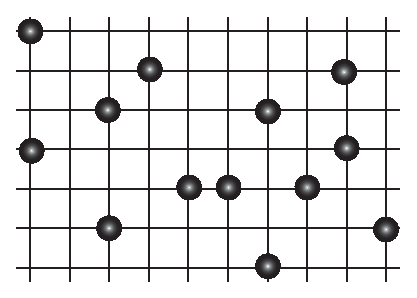
\includegraphics{./figures/FIG_LatticeModel.eps}
  \end{center}
\end{figure}
%

異なる格子点を占める粒子の間には相互作用はなく、粒子は格子点から格子点へと自由に移動することができるが、2 つ以上の粒子は同じ格子点を占めることはできないと仮定する。
1 つの格子点当たりの空間の体積を $v_0$ とすると、この系は体積が $V \equiv v_0 L$ の気体のモデルであると考えることができ、格子気体と呼ばれる。

この格子気体に関して、以下の設問に答えよ。

%なお、必要であれば、$N \gg 1$ のときに成立する Stirling の公式 $\ln N! \sim N \ln N - N$ は、証明なしで用いて構わない。

%\vspace{8pt}
\begin{enumerate}
\setlength{\parskip}{0cm} % 段落間
\setlength{\itemsep}{0.3cm} % 項目間

\item
この系のエントロピー $S$ および Helmholtz の自由エネルギー $F$ を求めよ。

\begin{itembox}[l]{{\bf ヒント:}}

ミクロカノニカル集団として取り扱えるので、エントロピーはボルツマンの関係式で導出でき、また、相互作用がないので、Helmholtz の自由エネルギー $F$ は、エントロピー項のみで記述できる。

また、必要に応じて、$N \gg 1$ のときに成立する Stirling の公式 $\ln N! \sim N \ln N - N$ を用いよ。
%\begin{align*}
%F=E-TS = -TS
%\end{align*}
\end{itembox}

\color{black}

\item
$L \gg N$ のときに、$N/L$ の項に対して $(N/L)^2$ の項を無視することで、この系の状態方程式が理想気体の状態方程式に一致することを示せ。
ただし、$\vert x \vert \ll 1$ のときの近似式 $\ln (1+x) \sim x$ は、証明なしで用いて構わない。

\begin{itembox}[l]{{\bf ヒント:}}

設問にあるように、格子点の総数 $L$ と、1 つの格子点当たりの空間の体積 $v_0$ から、この系の体積を $V \equiv v_0 L$ とみなす事ができる。

また、Helmholtz の自由エネルギー $F$ を体積で偏微分すると、以下のように圧力 $P$ を得る。
\begin{align*}
P = -\left( \dfrac{\partial F}{\partial V} \right)_{T,N} 
\end{align*}

\end{itembox}

\color{black}

\item
前問までは、すべてが同一の $N$ 粒子系を考えたが、今度は $N_A$ 個の $A$-粒子および $N_B$ 個の $B$-粒子からなる2成分系の場合に、エントロピー $S'$ の表式を求めよ。
ただし、$N_A + N_B = N$ とする。

\begin{itembox}[l]{{\bf ヒント:}}

この設問の場合、全系の微視的状態数 $W'$ は、総数が $L$ である空間格子上に同一の見分けの付かない $N_A$ をばらまいたうえで、残った格子上に、
$N_B$ 個の粒子をばらまく場合の組み合わせで表されることになる。

\end{itembox}

\item
ここまでに求めた一成分系のエントロピー $S$ と、二成分系のエントロピー $S'$ の差 $\Delta S \equiv S' - S$ の持つ物理的な意味を説明せよ。

\begin{itembox}[l]{{\bf ヒント:}}

差を具体的に算出したうえで、エントロピーの増加と不可逆過程について論ぜよ。

\end{itembox}

\color{black}

\end{enumerate}

\newpage

図に示すような空間格子(格子点の総数を $L$ とする)と、格子点上に分布する同一の見分けの付かない $N$ 個の粒子からなる系を考える。
($L$、$N \gg 1$ とする。) 
%
\begin{figure}[h]
  \begin{center}
    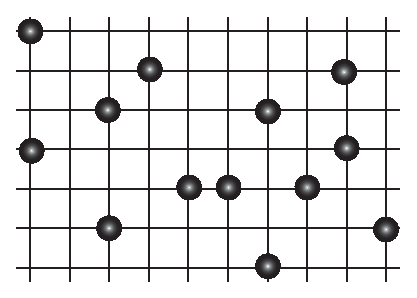
\includegraphics{./figures/FIG_LatticeModel.eps}
  \end{center}
\end{figure}
%

異なる格子点を占める粒子の間には相互作用はなく、粒子は格子点から格子点へと自由に移動することができるが、2 つ以上の粒子は同じ格子点を占めることはできないと仮定する。
1 つの格子点当たりの空間の体積を $v_0$ とすると、この系は体積が $V \equiv v_0 L$ の気体のモデルであると考えることができ、格子気体と呼ばれる。

この格子気体に関して、以下の設問に答えよ。

%なお、必要であれば、$N \gg 1$ のときに成立する Stirling の公式 $\ln N! \sim N \ln N - N$ は、証明なしで用いて構わない。

%\vspace{8pt}
\begin{enumerate}
\setlength{\parskip}{0cm} % 段落間
\setlength{\itemsep}{0.3cm} % 項目間

\item
この系のエントロピー $S$ および Helmholtz の自由エネルギー $F$ を求めよ。
\vspace{8pt}

\begin{itembox}[l]{{\bf ヒント:}}

ミクロカノニカル集団として取り扱えるので、エントロピーはボルツマンの関係式で導出でき、また、相互作用がないので、Helmholtz の自由エネルギー $F$ は、エントロピー項のみで記述できる。

また、必要に応じて、$N \gg 1$ のときに成立する Stirling の公式 $\ln N! \sim N \ln N - N$ を用いよ。
%\begin{align*}
%F=E-TS = -TS
%\end{align*}
\end{itembox}

\vspace{8pt}

{\bf (解答例)}

設問の条件から、この系はミクロカノニカル集団として取り扱うことが妥当であるので、求めるエントロピーは、微視的状態数を数え上げてボルツマンの関係式を用いることで導出できる
\footnote{
ミクロカノニカル集団に関する参考事項:\href{http://kisokouza.island.ac/documents/Stat_Phys_Entropy.pdf}{「統計力学エントロピー」の「4.3 ミクロカノニカル集団」}
}。

この設問の場合、排除体積効果を考慮するのであるから、微視的状態数は、総数が $L$ である空間格子上に同一の見分けの付かない $N$ 個の粒子を「重なり合わせなく」ばらまく場合の組み合わせ
\footnote{
「組み合わせ」に関する参考事項:\href{http://kisokouza.island.ac/documents/Permutation_Combination.pdf}{「順列」と「組み合わせ」の「3 組み合わせ(Combination)」}
}
ということになり、
\begin{align*}
W 
	&= {}_L C_N \\
	&= \dfrac{L!}{(L-N)! N!} 
\end{align*}
で表される。

したがって、求めるエントロピーは、ボルツマンの関係式から、
\begin{align*}
S 
	&= k_B \ln W \\
	&= k_B \ln \left[ \dfrac{L!}{(L-N)! N!} \right] \\
	&= k_B \left[ \ln L! - \ln (L-N)! - \ln N! \right] \\
	&\simeq k_B \left[ \{ L\ln L -L\} - \{ (L-N)\ln (L-N) - (L-N) \} - \{N\ln N -N \} \right] \\
	&= k_B \left[ L\ln L - (L-N)\ln (L-N) - N\ln N \right] 
\end{align*}
となる。

対象とする系は相互作用がないので、Helmholtz の自由エネルギー $F$ は、以下のように導出される。
\begin{align*}
F=E-TS = -TS = -k_B T \left[ L\ln L - (L-N)\ln (L-N) - N\ln N \right] 
\end{align*}

\newpage

\item
$L \gg N$ のときに、$N/L$ の項に対して $(N/L)^2$ の項を無視することで、この系の状態方程式が理想気体の状態方程式に一致することを示せ。
ただし、$\vert x \vert \ll 1$ のときの近似式 $\ln (1+x) \sim x$ は、証明なしで用いて構わない。

\vspace{8pt}

\begin{itembox}[l]{{\bf ヒント:}}

設問にあるように、格子点の総数 $L$ と、1 つの格子点当たりの空間の体積 $v_0$ から、この系の体積を $V \equiv v_0 L$ とみなす事ができる。

また、Helmholtz の自由エネルギー $F$ を体積で偏微分すると、以下のように圧力 $P$ を得る。
\begin{align*}
P = -\left( \dfrac{\partial F}{\partial V} \right)_{T,N} 
\end{align*}
\end{itembox}
%\vspace{8pt}

{\bf (解答例)}

設問にあるように、格子点の総数 $L$ と、1 つの格子点当たりの空間の体積 $v_0$ から、この系の体積を $V \equiv v_0 L$ とみなすと、
Helmholtz の自由エネルギー $F$ を体積で微分して圧力 $P$ を得る、以下の関係を用いて、
\begin{align*}
P = -\left( \dfrac{\partial F}{\partial V} \right)_{T,N} 
	&=
	\dfrac{1}{v_0}  k_B T \dfrac{\partial }{\partial L} \left[ L\ln L - (L-N)\ln (L-N) - N\ln N \right] \\
	&=
	\dfrac{k_B T}{v_0}  \left[ \{\ln L +1\} - \{\ln (L-N) + 1\} \right] \\
	&=
	\dfrac{k_B T}{v_0}  \ln \left(\dfrac{L}{L-N} \right) \\	
	&=
	-\dfrac{k_B T}{v_0}  \ln \left(\dfrac{L-N}{L} \right) \\
	&=
	-\dfrac{k_B T}{v_0}  \ln \left(1-\dfrac{N}{L} \right) \\
	&\simeq
	-\dfrac{k_B T}{v_0} \left(-\dfrac{N}{L} \right) \\
	&= 	-\dfrac{N k_B T}{V}
\end{align*}
なお、六行目への展開では、対数のテイラー展開を用いている
\footnote{
ここでは、対数のテイラー展開($\ln \left(1 + x \right) = x - \dfrac{x^2}{2} + \dfrac{x^3}{3} -\dots$)を利用して、さらに、設問の条件に従い二次の項以降を無視することで、以下の展開を行っている。
\begin{align*}
\ln \left(1 - \dfrac{N}{L} \right) 
	&= 
	\left[ \left (- \dfrac{N}{L} \right) - \dfrac{\left (- \dfrac{N}{L} \right)^2}{2} \right] \\
	&= \left (- \dfrac{N}{L} \right)
\end{align*}
}。

したがって、以下の理想気体の状態方程式を得る。
\begin{equation*}
PV = N k_B T
\end{equation*}

\newpage

\item
前問までは、すべてが同一の $N$ 粒子系を考えたが、今度は $N_A$ 個の $A$-粒子および $N_B$ 個の $B$-粒子からなる2成分系の場合に、エントロピー $S'$ の表式を求めよ。
ただし、$N_A + N_B = N$ とする。

\vspace{8pt}

\begin{itembox}[l]{{\bf ヒント:}}

この設問の場合、全系の微視的状態数 $W'$ は、総数が $L$ である空間格子上に同一の見分けの付かない $N_A$ をばらまいたうえで、残った格子上に、
$N_B$ 個の粒子をばらまく場合の組み合わせで表されることになる。

\end{itembox}
%\vspace{8pt}

{\bf (解答例)}

この設問の場合、全系の微視的状態数 $W'$ は、総数が $L$ である空間格子上に同一の見分けの付かない $N_A$ をばらまいたうえで、残った格子上に、
$N_B$ 個の粒子をばらまく場合の組み合わせで表されることになり、
\begin{align*}
W' 
	&= {}_L C_{N_A} \times {}_{(L-N_A)} C_{N_B} \\
	&= \dfrac{L!}{(L-N_A)! N_A!} \times \dfrac{(L-N_A)!}{(L-N_A-N_B)! N_B!} \\
	&= \dfrac{L!}{(L-N_A-N_B)! N_A! N_B!} 
\end{align*}
で表される。

したがって、求めるエントロピーは、ボルツマンの関係式から、
\begin{align*}
S' 
	&= k_B \ln W' \\
	&= k_B \ln \left[ \dfrac{L!}{(L-N_A-N_B)! N_A! N_B!} \right] \\
	&= k_B \left[ \ln L! - \ln (L-N_A-N_B)! - \ln N_A! - \ln N_B! \}\right] \\
	&\simeq k_B \left[ \{ L\ln L -L\} - \{ (L-N_A-N_B)\ln (L-N_A-N_B) - (L-N_A -N_B) \} \right. \\
	&\quad \left. - \{N_A\ln N_A -N_A \} - \{N_B\ln N_B -N_B \} \right] \\
	&= k_B \left[ L\ln L - (L-N)\ln (L-N) - N_A\ln N_A - N_B\ln N_B \right]
\end{align*}
となる。


\newpage

\item
ここまでに求めた一成分系のエントロピー $S$ と、二成分系のエントロピー $S'$ の差 $\Delta S \equiv S' - S$ の持つ物理的な意味を説明せよ。

\begin{itembox}[l]{{\bf ヒント:}}

差を具体的に算出したうえで、エントロピーの増加と不可逆過程について論ぜよ。

\end{itembox}

{\bf (解答例)}

それぞれのエントロピーの差は、以下のようになる。
\begin{align*}
\Delta S 
	&= k_B \left[ L\ln L - (L-N)\ln (L-N) - N_A\ln N_A - N_B\ln N_B \right] \\
	&\quad - k_B \left[ L\ln L - (L-N)\ln (L-N) - N\ln N \right] \\
	&= k_B [N_A ( \ln N - \ln N_A) + N_B ( \ln N - \ln N_B)] \\
	&= N_A k_B \ln \left( \dfrac{N}{N_A} \right) + N_B k_B \ln \left( \dfrac{N}{N_B} \right)
\end{align*}

異種混合の場合には、同種混合に比べて上記の $\Delta S$ だけ混合によるエントロピー増加が生じている。
これは、「異種の粒子を混合した場合、一様に混合することでエントロピーを増加できること」、すなわち、不可逆過程として混合が進行することを表している。

\end{enumerate}


\newpage

%**********************************************************************
%                              問4
%**********************************************************************
\subsubsection{結晶格子の二準位系モデル}

\begin{boxnote}
{\bf 出題意図:}
二準位系と呼ばれる、相互作用のないスピン系に相当する系の平衡状態をカノニカル集団の方法を用いて計算する問題です。
基本的に前問の格子気体と似た振る舞いを示します。
\end{boxnote}
\vspace{8pt}

結晶格子点上に $N$ 個の同一の原子が配置されている。
それぞれの原子は、エネルギーが $0$ の基底状態とエネルギーが $\epsilon (>0)$ の励起状態の2つの状態だけを取ることができるとする。

原子間には相互作用がないものとして、以下の設問に答えよ。

%\vspace{8pt}
\begin{enumerate}
\setlength{\parskip}{0cm} % 段落間
\setlength{\itemsep}{0.3cm} % 項目間

\item
系が温度 $T$ の熱浴に接していると仮定して、古典カノニカル統計を適用する。

この系の1粒子状態和 $z$ および全系の状態和 $Z$ を求め、系のヘルムホルツ自由エネルギー $F$ を求めよ。

\begin{itembox}[l]{{\bf ヒント:}}

エネルギーが $0$ の基底状態のボルツマン因子は、$\exp(-\beta \times 0) = 1$ であり、エネルギーが $\epsilon (>0)$ の励起状態のボルツマン因子は、$\exp(-\beta \times \epsilon)$ である。
また、相互作用のない二準位理想系の一粒子状態和は、それぞれのボルツマン因子の和となることを用いよ。

\end{itembox}

\color{black}

\item
任意に1つの原子に目を付けたときに、この原子が基底状態および励起状態のそれぞれのエネルギー準位を占める確率 $P_0$ および $P_{\epsilon}$ を求めよ。

\begin{itembox}[l]{{\bf ヒント:}}

それぞれの状態のボルツマン因子を前問で求めた一粒子状態和で割れば、その状態を占める確率となることを用いればよい。

\end{itembox} 

\color{black}

\item
温度一定の平衡状態においては、決して $P_0 < P_{\epsilon}$ とならないことを示せ。
また、その理由を直感的に説明せよ。

\begin{itembox}[l]{{\bf ヒント:}}

実際に差を計算し、一般的なカノニカル分布では必ずしもエネルギーの低い状態の出現確率が高いわけではないこととの比較を行えばよい。

\end{itembox}

\color{black}

\end{enumerate}

\newpage

結晶格子点上に $N$ 個の同一の原子が配置されている。
それぞれの原子は、エネルギーが $0$ の基底状態とエネルギーが $\epsilon (>0)$ の励起状態の2つの状態だけを取ることができるとする。

原子間には相互作用がないものとして、以下の設問に答えよ。

%\vspace{8pt}
\begin{enumerate}
\setlength{\parskip}{0cm} % 段落間
\setlength{\itemsep}{0.3cm} % 項目間

\item
系が温度 $T$ の熱浴に接していると仮定して、古典カノニカル統計を適用する。

この系の1粒子状態和 $z$ および全系の状態和 $Z$ を求め、系のヘルムホルツ自由エネルギー $F$ を求めよ。
\vspace{8pt}

\begin{itembox}[l]{{\bf ヒント:}}

エネルギーが $0$ の基底状態のボルツマン因子は、$\exp(-\beta \times 0) = 1$ であり、エネルギーが $\epsilon (>0)$ の励起状態のボルツマン因子は、$\exp(-\beta \times \epsilon)$ である。
また、相互作用のない二準位理想系の一粒子状態和は、それぞれのボルツマン因子の和となることを用いよ。

\end{itembox}

{\bf (解答例)}

相互作用のない二準位理想系(エネルギーが $0$ の基底状態とエネルギーが $\epsilon (>0)$ の励起状態)であるため、一粒子状態和は、
\begin{align*}
z 
	&= [\exp(-\beta \times 0) + \exp(-\beta \times \epsilon)] \\
	&= [1 + \exp(-\beta \epsilon)]
\end{align*}
と書くことができる
\footnote{
状態和に関する参考事項:\href{http://kisokouza.island.ac/documents/Stat_Phys_Entropy.pdf}{「統計力学エントロピー」の「4.4.3 古典理想系でのカノニカル集団」}
}。

このとき、結晶格子点上の $N$ 個の同一の原子が対象とする系であるので、見分けのつく古典系と考え、全系の状態和は、以下のように書ける。
\begin{equation*}
Z = \Pi_i z_i = [1 + \exp(-\beta \epsilon)]^N
\end{equation*}

したがって、ヘルムホルツの自由エネルギーは、
\begin{equation*}
F = - k_BT \ln Z = -N k_B T \ln  [1 + \exp(-\beta \epsilon)]
\end{equation*}
\newpage

\item
任意に1つの原子に目を付けたときに、この原子が基底状態および励起状態のそれぞれのエネルギー準位を占める確率 $P_0$ および $P_{\epsilon}$ を求めよ。
\vspace{8pt}

\begin{itembox}[l]{{\bf ヒント:}}

それぞれの状態のボルツマン因子を前問で求めた一粒子状態和で割れば、その状態を占める確率となることを用いればよい。

\end{itembox} 

{\bf (解答例)}

それぞれの状態のボルツマン因子を一粒子状態和で除して、求める確率は以下のように算出できる。
\begin{equation*}
\begin{cases}
P_0 = \dfrac{1}{z} \exp(-\beta \times 0) = \dfrac{1}{1 + \exp(-\beta \epsilon)} \\[10pt]
P_{\epsilon} = \dfrac{1}{z} \exp(-\beta \times \epsilon) = \dfrac{\exp(-\beta \epsilon)}{1 + \exp(-\beta \epsilon)}
\end{cases}
\end{equation*}

\newpage

\item
温度一定の平衡状態においては、決して $P_0 < P_{\epsilon}$ とならないことを示せ。
また、その理由を直感的に説明せよ。
\vspace{8pt}

\begin{itembox}[l]{{\bf ヒント:}}

実際に差を計算し、一般的なカノニカル分布では必ずしもエネルギーの低い状態の出現確率が高いわけではないこととの比較を行えばよい。

\end{itembox}

{\bf (解答例)}

$P_0 - P_{\epsilon} $ は、以下のように展開できる。
\begin{align*}
P_0 - P_{\epsilon} 
	&= \dfrac{1}{1 + \exp(-\beta \epsilon)} - \dfrac{\exp(-\beta \epsilon)}{1 + \exp(-\beta \epsilon)} \\[10pt]
	&= \dfrac{1 - \exp(-\beta \epsilon)}{1 + \exp(-\beta \epsilon)}
\end{align*}

古典統計の範囲では、いかなる $\epsilon$ に対しても、$-\beta \epsilon < 0$ であるから、 $\exp(-\beta \epsilon) < 1$ となり、常に、$P_0 - P_{\epsilon} >0$ で、$P_0 > P_{\epsilon}$ であり、決して $P_0 < P_{\epsilon}$ とはならない。 

カノニカル統計においては、エントロピーの寄与により、単純にエネルギーが低い状態が多く出現するとは必ずしも限らない。

ここで対象とした 2 準位系ではエネルギー 0 の状態とエネルギー $\epsilon$ の状態はそれぞれ縮退していないので、単純にボルツマン因子に出現確率が比例することになり、
このため、エネルギーの高い状態の方が「必ず」出現確率が低くなる。

\color{black}

\end{enumerate}

\newpage


%**********************************************************************
%                              問5
%**********************************************************************

\subsubsection{高分子一次元モデル}

\begin{boxnote}
{\bf 出題意図:}
高分子のモデルとして一次元の連鎖を考え、その微視的状態数から系のエントロピーを求める問題です。
この問題は、二準位系の問題の特殊な場合(二つの準位のエネルギーが同じ)になっています。
\end{boxnote}
\vspace{8pt}
同一かつ互いに見分けのつく $N$ 個の粒子からなる1次元的な連鎖を考える。
粒子間には相互作用はなく、各粒子はエネルギーが同一の値 $\epsilon$ を持つ縮退した 2 つの状態 A および B のいずれかを互いに独立に取れるものとする。
このとき、以下の設問に答えよ。


\begin{enumerate}
\setlength{\parskip}{0cm} % 段落間
\setlength{\itemsep}{0.3cm} % 項目間

\item
状態 A にいる粒子の数が $n$ であるときに、ミクロカノニカル集団の方法を用いて、全系の微視的状態の総数 $W(n)$ が、$W(n) = N!/[ n! (N-n)!]$ で与えられることを示せ。

\begin{itembox}[l]{{\bf ヒント:}}

全系の微視的状態数 $W(n)$ は、総数 $N$ から、状態 A にいる粒子を $n$ 個選び取る「場合の数」になる。
なぜなら、状態 A にいる粒子を選び取った後では、残った粒子を状態 B に選ぶ場所はユニークに決まってしまう。

\end{itembox}

\color{black}

\item
$N \gg 1$ のとき、上の結果を用いてエントロピー $S(n)$ および Helmholtz 自由エネルギー $F(n)$ を求めよ。

\begin{itembox}[l]{{\bf ヒント:}}

エントロピー $S(n)$ は、上記の微視的状態数から、ボルツマンの関係式により導出でき、 Helmholtz 自由エネルギー $F(n)$ は相互作用エネルギーがないのであるから、以下となる。
\begin{align*}
F(n) = E - TS(n) = -TS(n)
\end{align*}

\end{itembox}

\color{black}

\item
図のように $N+1$ 個の粒子を、左右自由に向きを変えることのできる $N$ 個の結合(長さ $b$ とする)でつないだ1次元的な鎖を考える($N \gg 1$)。

\begin{figure}[h]
	\begin{center}
	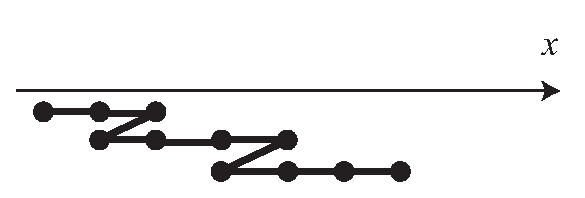
\includegraphics{./figures/FIG_chain.eps}
	\end{center}
\end{figure}
手前の粒子に対して、次の粒子が右側にいるか左側にいるかの2つの状態を、設問の2つの状態 A と B と見なすことにする。
設問 (a) の結果を利用して、この鎖の両端間の距離が $Mb$ であるときに、両端間に作用する熱力学的な力(張力に相当)を求めよ。

\begin{itembox}[l]{{\bf ヒント:}}

ただし、両端間距離を変数 $x$ で表すとき、両端間に作用する熱力学的な力 $f$ は、Helmholtz 自由エネルギー $F$ を用いて $f = (\partial F(x)/\partial x)_T$ で与えられる。
(すなわち体積と圧力の関係と同様であるが、圧力と張力では作用する方向が逆である。)

\end{itembox}

\color{black}

\end{enumerate}

\newpage


同一かつ互いに見分けのつく $N$ 個の粒子からなる1次元的な連鎖を考える。
粒子間には相互作用はなく、各粒子はエネルギーが同一の値 $\epsilon$ を持つ縮退した 2 つの状態 A および B のいずれかを互いに独立に取れるものとする。
このとき、以下の設問に答えよ。

\begin{enumerate}
\setlength{\parskip}{0cm} % 段落間
\setlength{\itemsep}{0.3cm} % 項目間

\item
状態 A にいる粒子の数が $n$ であるときに、ミクロカノニカル集団の方法を用いて、全系の微視的状態の総数 $W(n)$ が、$W(n) = N!/[ n! (N-n)!]$ で与えられることを示せ。
\vspace{8pt}

\begin{itembox}[l]{{\bf ヒント:}}

全系の微視的状態数 $W(n)$ は、総数 $N$ から、状態 A にいる粒子を $n$ 個選び取る「場合の数」になる。
なぜなら、状態 A にいる粒子を選び取った後では、残った粒子を状態 B に選ぶ場所はユニークに決まってしまう。

\end{itembox}

{\bf (解答例)}

状態 A にいる粒子の数が $n$ であるから、状態 B にいる粒子の数は $N-n$ となる。

この設問の場合、全系の微視的状態数 $W(n)$ は、総数 $N$ から、状態 A にいる粒子を $n$ 個選び取る場合の数となる。
なぜなら、状態 A にいる粒子を選び取った後では、残った粒子を状態 B に選ぶ場所はユニークに決まってしまうからである。
\begin{align*}
W(n) 
	&= {}_N C_{n} \\
	&= \dfrac{N!}{(N-n)! n!}
\end{align*}
で表される。

\newpage

\item
$N \gg 1$ のとき、上の結果を用いてエントロピー $S(n)$ および Helmholtz 自由エネルギー $F(n)$ を求めよ。
\vspace{8pt}

\begin{itembox}[l]{{\bf ヒント:}}

エントロピー $S(n)$ は、上記の微視的状態数から、ボルツマンの関係式により導出でき、 Helmholtz 自由エネルギー $F(n)$ は相互作用エネルギーがないのであるから、以下となる。
\begin{align*}
F(n) = E - TS(n) = -TS(n)
\end{align*}

\end{itembox}

{\bf (解答例)}

エントロピー $S(n)$ は、上記の微視的状態数から、ボルツマンの関係式により、
\begin{align*}
S(n) 
	&= k_B \ln W(n) \\
	&= k_B \ln \dfrac{N!}{(N-n)! n!} \\
	&\simeq k_B [ \{N\ln N - N \} - \{(N-n) \ln (N-n) - (N-n) \} - \{n\ln n -n\} ] \\
	&= k_B [ N\ln N  - (N-n) \ln (N-n)  - n\ln n ]
\end{align*}
なお、三行目へは、スターリングの公式($\ln N! \simeq N \ln N - N$)を用いた。

対象とする系は相互作用がないので、Helmholtz の自由エネルギー $F(n)$ は、以下のように導出される。
\begin{align*}
F(n) = E - TS(n) = -TS(n) = -k_B T [ N\ln N  - (N-n) \ln (N-n)  - n\ln n ] 
\end{align*}

\newpage

\item
図のように $N+1$ 個の粒子を、左右自由に向きを変えることのできる $N$ 個の結合(長さ $b$ とする)でつないだ1次元的な鎖を考える($N \gg 1$)。

\begin{figure}[h]
	\begin{center}
	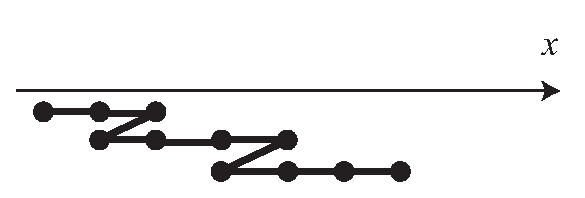
\includegraphics{./figures/FIG_chain.eps}
	\end{center}
\end{figure}
手前の粒子に対して、次の粒子が右側にいるか左側にいるかの2つの状態を、設問の2つの状態 A と B と見なすことにする。
設問 (a) の結果を利用して、この鎖の両端間の距離が $Mb$ であるときに、両端間に作用する熱力学的な力(張力に相当)を求めよ。
\vspace{8pt}

\begin{itembox}[l]{{\bf ヒント:}}

ただし、両端間距離を変数 $x$ で表すとき、両端間に作用する熱力学的な力 $f$ は、Helmholtz 自由エネルギー $F$ を用いて $f = (\partial F(x)/\partial x)_T$ で与えられる。
(すなわち体積と圧力の関係と同様であるが、圧力と張力では作用する方向が逆である。)

\end{itembox}

{\bf (解答例)}

この設問の場合、粒子間をつなぐボンドの向きを考えることにする。
鎖の両端間の距離が $Mb$ となるということは、状態 A となるボンドの数 $n_A$ が、状態 B となるボンドの数 $n_B$ よりも $M$ 個分だけ偏っている(多い、あるいは少ない)ということである。
このとき、それぞれの粒子の数は、以下となる。
\begin{equation*}
\begin{cases}
n_A = \dfrac{N+M}{2} \\[10pt]
n_B = \dfrac{N-M}{2}
\end{cases}
\end{equation*}

このとき、ボンドの微視的状態数 $W$ は、ボンドの総数 $N$ から、状態 A であるボンドの数だけ選び取り、残りを状態 B に選び出すという「組み合わせ」の積で表されることになり、
\begin{align*}
W 
	&= {}_N C_{n_A} \times {}_{(N-n_A)} C_{n_B} \\
	&= \dfrac{N!}{(N-n_A)! n_A!} \times \dfrac{(N-n_A)!}{0! (n_B)!} \\
	&= \dfrac{N!}{ \left( \dfrac{N}{2}-\dfrac{M}{2} \right)! \left( \dfrac{N}{2}+\dfrac{M}{2} \right)!}
\end{align*}
で表される。

したがって、エントロピーは、
\begin{align*}
S 
	&= k_B \ln W \\
	&= k_B \ln \left[ \dfrac{N!}{ \left( \dfrac{N}{2}-\dfrac{M}{2} \right)! \left( \dfrac{N}{2}+\dfrac{M}{2} \right)!} \right] \\
	&= k_B \left[ \ln N! -\ln \left( \dfrac{N}{2}-\dfrac{M}{2} \right)! -\ln \left( \dfrac{N}{2}+\dfrac{M}{2} \right)! \right]\\
	&= k_B \left[ \{ N\ln N - N \} - \left\{ \left( \dfrac{N}{2}-\dfrac{M}{2} \right)\ln \left( \dfrac{N}{2}-\dfrac{M}{2} \right) -\left( \dfrac{N}{2}-\dfrac{M}{2} \right) \right\} \right. \\
	&\quad \left. - \left\{ \left( \dfrac{N}{2}+\dfrac{M}{2} \right) \ln \left( \dfrac{N}{2}+\dfrac{M}{2} \right) - \left( \dfrac{N}{2}+\dfrac{M}{2} \right) \right\} \right]\\
	&= k_B \left[ N\ln N - \left( \dfrac{N}{2}-\dfrac{M}{2} \right)\ln \left( \dfrac{N}{2}-\dfrac{M}{2} \right) - \left( \dfrac{N}{2}+\dfrac{M}{2} \right) \ln \left( \dfrac{N}{2}+\dfrac{M}{2} \right) \right]\\
	&= k_B \left[ N\ln N - \dfrac{N}{2} \ln \left( \dfrac{N}{2}-\dfrac{M}{2} \right)\left( \dfrac{N}{2}+\dfrac{M}{2} \right) 
	+\dfrac{M}{2} \ln \dfrac{\left( \dfrac{N}{2}-\dfrac{M}{2} \right)}{ \left( \dfrac{N}{2}+\dfrac{M}{2} \right) } \right]  \\
	&= k_B \left[ N\ln N - \dfrac{N}{2} \ln \left( \dfrac{N^2}{4}-\dfrac{M^2}{4} \right) 
	+\dfrac{M}{2} \ln \dfrac{N - M}{ N+M } \right]  \\
	&= k_B \left[ N\ln N - \dfrac{N}{2} \ln \left\{ \dfrac{N^2}{4}\left(1-\dfrac{M^2}{N^2} \right) \right\} 
	+\dfrac{M}{2} \ln \left( 1 - \dfrac{2M}{N+M} \right) \right]  \\
	&= k_B \left[ N\ln N - \dfrac{N}{2} \ln \dfrac{N^2}{4} - \dfrac{N}{2} \ln \left(1-\dfrac{M^2}{N^2} \right) 
	+\dfrac{M}{2} \ln \left( 1 - \dfrac{2M}{N+M} \right) \right]  \\
	&\simeq k_B \left[ N\ln N - \dfrac{N}{2} \ln \dfrac{N^2}{4} - \dfrac{N}{2}\left(-\dfrac{M^2}{N^2} \right) 
	+\dfrac{M}{2} \left(- \dfrac{2M}{N+M} \right) \right]  \\
	&= k_B \left( N\ln N - \dfrac{N}{2} \ln \dfrac{N^2}{4} + \dfrac{M^2}{2N} -\dfrac{M^2}{N+M} \right) \\
	&= k_B \left( N\ln N - \dfrac{N}{2} \ln \dfrac{N^2}{4} + \dfrac{M^2}{2N} -\dfrac{M^2}{N} \right) \\
	&= k_B \left( N\ln N - \dfrac{N}{2} \ln \dfrac{N^2}{4} - \dfrac{M^2}{2N} \right)
\end{align*}
なお、10 行目への展開において、$N \gg M$ と仮定して、対数のテイラー展開を一次の項で打ち切る近似($\ln(1+x) \simeq x$)を行い、さらに11行目で、$\dfrac{M^2}{N+M} = \dfrac{M^2}{N}$ という近似も行った。

このとき、Helmholtz の自由エネルギー $F$ は、以下のように導出される。
\begin{align*}
F 	&= E - TS \\
	&= -TS \\
	&= -k_B T \left( N\ln N - \dfrac{N}{2} \ln \dfrac{N^2}{4} - \dfrac{M^2}{2N} \right) \\
	&= -k_B T \left( N\ln N - \dfrac{N}{2} \ln \dfrac{N^2}{4} - \dfrac{x^2}{2Nb^2} \right) 
\end{align*}
なお、末端間距離 $x$ が $Mb$ と等しいことから $M = \dfrac{x}{b}$ となるので上式に代入している。

したがって、求める張力は、
\begin{align*}
f 	&= \left(\dfrac{\partial F(x)}{\partial x} \right)_T \\
	&=\dfrac{\partial}{\partial x} \left[ -k_B T \left( N\ln N - \dfrac{N}{2} \ln \dfrac{N^2}{4} - \dfrac{x^2}{2Nb^2} \right) \right]\\
	&=- \dfrac{k_B T x}{Nb^2}
\end{align*}
となる。

\end{enumerate}

\newpage


























\section{高分子物理}

\subsection{高分子鎖の静的性質}

\subsubsection{理想鎖の末端間距離}

\begin{boxnote}
いろいろなボンドのモデルを用いて構成された高分子鎖の末端間距離の 2 乗の確率分布を計算することで、高分子の空間的な広がりの分布が、
どのようなボンドのモデルを用いたかには依らないユニバーサルな性質を示すことを確認する問題です。
確率変数の独立性の復習にもなっています。
\end{boxnote}

\vspace{10pt}

以下に示すような種々の高分子鎖のモデルを用いて、$N+1$ 個のビーズ(あるいは格子点)の連鎖からなる高分子鎖の末端間の平均 2 乗距離 $\langle R^2 \rangle$ を計算してみよう。

ただし、ビーズは互いに重なることを許す理想鎖の統計を考えることとする。


%\vspace{10pt}

\begin{enumerate}
\setlength{\parskip}{0cm} % 段落間
\setlength{\itemsep}{0.5cm} % 項目間
\item
格子定数 a の立方格子上の連続する $N + 1$ 個の格子点を結んでできた鎖。
%\vspace{8pt}
\begin{itembox}[l]{{\bf ヒント:}}

 隣り合うビーズ(あるいは格子点)を結ぶボンドベクトルを、$\bm{u}_i (i = 1, 2, \cdots, N)$ とすると、異なるボンドの方向は無相関になるので、
$\langle \bm{u}_i \cdot \bm{u}_j \rangle = 0 \; ( i \neq j \text{のとき})$ が成立する。
\end{itembox}

\item 
長さが a  (一定とする)で自由に回転することのできる剛体棒でつながれた $N+1$ 個のビーズの連鎖から構成される鎖。

%\vspace{8pt}
\begin{itembox}[l]{{\bf ヒント:}}

この場合には ボンドの方向が等方的に分布しているという点が上記の格子モデルとは異なるが、それ以外の性質(異なるボンドの統計的な独立性やボンド長固定の性質)は共通なので、格子モデルの場合とまったく同様な考え方で取り扱うことができる。

\end{itembox}


\item
ボンドベクトル $\bm{u}$ の方向はランダムで、長さ $u = |\bm{u}|$ が確率分布 $P(u)$ に従うようなボンドで結ばれた $N+1$ 個のビーズから構成される鎖。

%\vspace{8pt}
\begin{itembox}[l]{{\bf ヒント:}}

この場合、ボンドベクトルの場合分けは同様であるが、ボンド長に確率分布を取り入れて以下のように記述されることになる。
\begin{align*}
\langle \bm{u}_i \cdot \bm{u}_j \rangle 
%	&= \langle \bm{\hat{u}}_i \cdot \bm{\hat{u}}_j \rangle \{uP(u)\}^2 \\
	&=
\begin{cases}
\langle |\bm{u}_i |^2 \rangle = \displaystyle \int d \bm{u}  \vert \bm{u} \vert^2 P(\bm{u}) 	&\quad (\text{$i = j$ のとき}) \\
\langle \bm{u}_i \rangle \cdot \langle \bm{u}_j \rangle = \bm{0}\cdot\bm{0} = 0	&\quad(\text{$i \neq j$ のとき})
\end{cases}
\end{align*}
\end{itembox}

\vspace{10pt}

\end{enumerate}

\newpage

\begin{enumerate}
\setlength{\parskip}{0cm} % 段落間
\setlength{\itemsep}{0.5cm} % 項目間

\item
格子定数 a の立方格子上の連続する $N + 1$ 個の格子点を結んでできた鎖。

\vspace{10pt}
\begin{itembox}[l]{{\bf ヒント:}}
隣り合うビーズ(あるいは格子点)を結ぶボンドベクトルを、$\bm{u}_i (i = 1, 2, \cdots, N)$ とすると、異なるボンドの方向は無相関になるので、
$\langle \bm{u}_i \cdot \bm{u}_j \rangle = 0 \; ( i \neq j \text{のとき})$ が成立する。
\end{itembox}

\vspace{10pt}

{\bf (解答例)}

鎖が配置される $N+1$ 個のそれぞれの格子点に、端から $0, 1, 2, \cdots, N-1, N$ とインデックスを付け、さらに、その格子点を隣接する格子点とつなぐボンド($N$ 個)にも同様に、 $0, 1, 2, \cdots, N-1$ と番号付けする。
ここで、$i$ 番目の格子点の位置ベクトルを $\bm{r}_i$ とすると、$i$ 番目のボンドを表すベクトルは、
\begin{equation*}
\bm{u}_i \equiv \bm{r}_{i+1} -\bm{r}_i \quad (i=0, 1, 2, \cdot, N-1)
\end{equation*}
で定義される。

立方格子では、各格子点は 6 個の格子点と隣接(最近接格子点と呼ばれる)することになる。
この設問では、理想鎖を対象としているので、各ボンドは完全に無相関で同じ格子点へと戻ることを許容する(排除体積がない)モデルとなっている。
このとき、各ボンドベクトルの間には、ヒントにあるように、以下に示した関係が成立する。
\begin{align*}
\langle \bm{u}_i \cdot \bm{u}_j \rangle 
	&= \langle \bm{\hat{u}}_i \cdot \bm{\hat{u}}_j \rangle a^2 \\
	&=
\begin{cases}
\langle |\bm{\hat{u}}_i |^2 \rangle a^2 = a^2	&\quad (\text{$i = j$ のとき}) \\
\langle \bm{u}_i \rangle \cdot \langle \bm{u}_j \rangle = \bm{0}\cdot\bm{0} = 0	&\quad(\text{$i \neq j$ のとき})
\end{cases}
\end{align*}
ここで、$\bm{\hat{u}}_i \equiv \dfrac{\bm{u}_i}{|\bm{u}_i|}$ は $\bm{u}_i$ 方向の単位ベクトル、$a$ はボンドの長さを表している。

このとき、$0$ 番目の格子点からスタートして、$N$ 番目の鎖末端に至る高分子鎖の配位は、格子点の位置ベクトルの集合 $\{\bm{r}_i\} \equiv \{ \bm{r}_0, \bm{r}_1, \cdots, \bm{r}_N \}$ 、あるいは、ボンドベクトルの集合 $\{\bm{u}_i\} \equiv \{ \bm{u}_0, \bm{u}_1, \cdots, \bm{u}_{N-1} \}$ で指定されることになる。


鎖の末端間ベクトル $\bm{R}$ は、
\begin{equation*}
\bm{R} \equiv \bm{r}_N - \bm{r}_0
\end{equation*}
で定義され、平均二乗末端間距離 $R^2$ は、このベクトルの大きさの二乗のアンサンブル平均として、以下のように展開できる。
\begin{align*}
R^2 
	&\equiv \left \langle \left | \bm{R} \right |^2 \right \rangle \\
	&= \left \langle \left | \bm{r}_N - \bm{r}_0 \right |^2 \right \rangle \\
	&= \left \langle \left | (\bm{r}_1 - \bm{r}_0) + (\bm{r}_2 - \bm{r}_1) + \cdots + (\bm{r}_N - \bm{r}_{N-1}) \right |^2 \right \rangle \\
	&= \left \langle \left| \sum_{i=0}^{N-1} \bm{u}_{i} \right|^2 \right\rangle \\
	&= \sum_{i=0}^{N-1} \left \langle \left| \bm{u}_{i} \right|^2 \right\rangle + \sum_{i \neq j} \left \langle \bm{u}_{i} \cdot \bm{u}_{j} \right\rangle \\
	&= N a^2
\end{align*}
なお、最後の行へは前述の理想鎖でのボンドベクトルの関係($\langle \left| \bm{u}_{i} \right|^2 \rangle = a^2$ および $\langle \bm{u}_{i} \cdot \bm{u}_{j} \rangle = 0$)を利用した。

\newpage

\item 
長さが a  (一定とする)で自由に回転することのできる剛体棒でつながれた $N+1$ 個のビーズの連鎖から構成される鎖。

%\vspace{8pt}
\begin{itembox}[l]{{\bf ヒント:}}

この場合には ボンドの方向が等方的に分布しているという点が上記の格子モデルとは異なるが、それ以外の性質(異なるボンドの統計的な独立性やボンド長固定の性質)は共通なので、格子モデルの場合とまったく同様な考え方で取り扱うことができる。

\end{itembox}

{\bf (解答例)}

ここに提示された自由回転鎖においても、それぞれのボンドは等方的に振る舞い、かつ、ボンド長は固定されているため、ボンドベクトルの性質は上記の格子モデルとまったく同一となる。

したがって、平均二乗末端間距離 $R^2$ は、
\begin{align*}
R^2 
= N a^2
\end{align*}
となる。

\newpage

\item
ボンドベクトル $\bm{u}$ の方向はランダムで、長さ $u = |\bm{u}|$ が確率分布 $P(u)$ に従うようなボンドで結ばれた $N+1$ 個のビーズから構成される鎖。

\vspace{10pt}
\begin{itembox}[l]{{\bf ヒント:}}

この場合、ボンドベクトルの場合分けは同様であるが、ボンド長に確率分布を取り入れて以下のように記述されることになる。
\begin{align*}
\langle \bm{u}_i \cdot \bm{u}_j \rangle 
%	&= \langle \bm{\hat{u}}_i \cdot \bm{\hat{u}}_j \rangle \{uP(u)\}^2 \\
	&=
\begin{cases}
\langle |\bm{u}_i |^2 \rangle = \displaystyle \int d \bm{u}  \vert \bm{u} \vert^2 P(\bm{u}) 	&\quad (\text{$i = j$ のとき}) \\
\langle \bm{u}_i \rangle \cdot \langle \bm{u}_j \rangle = \bm{0}\cdot\bm{0} = 0	&\quad(\text{$i \neq j$ のとき})
\end{cases}
\end{align*}
\end{itembox}


{\bf (解答例)}

提示されたボンドは、等方的な振る舞いはこれまでのモデルと同等であるがボンド長が確率分布に従って変化する。
%ボンド長の期待値は $uP(u)$ であるので、$i$ 番目のボンドベクトル $\bm{u}_i$ は、その単位ベクトル $\bm{\hat{u}}_i$ と確率分布との積で、
%\begin{equation*}
%\bm{u}_i = \bm{\hat{u}}_i uP(u)
%\end{equation*}
%と書くことができる。
%
%したがって

このとき、ボンドベクトルの性質は以下のように記述されることになる。
\begin{align*}
\langle \bm{u}_i \cdot \bm{u}_j \rangle 
%	&= \langle \bm{\hat{u}}_i \cdot \bm{\hat{u}}_j \rangle \{uP(u)\}^2 \\
	&=
\begin{cases}
\langle |\bm{u}_i |^2 \rangle = \displaystyle \int d \bm{u}  \vert \bm{u} \vert^2 P(\bm{u}) 	&\quad (\text{$i = j$ のとき}) \\
\langle \bm{u}_i \rangle \cdot \langle \bm{u}_j \rangle = \bm{0}\cdot\bm{0} = 0	&\quad(\text{$i \neq j$ のとき})
\end{cases}
\end{align*}
なお、インデックスが等しいときの表式はボンドベクトルの長さの二乗平均を表すものであり、「ボンドベクトル $\bm{u}$ についての分布関数 $P(\bm{u})$ の分散」と考えることができる。

したがって、平均二乗末端間距離 $R^2$ は、
\begin{align*}
R^2 
	&\equiv \left \langle \left | \bm{R} \right |^2 \right \rangle \\
	&
%\vdots \\
	= \left \langle \left | \bm{r}_N - \bm{r}_0 \right |^2 \right \rangle \\
	&= \left \langle \left | (\bm{r}_1 - \bm{r}_0) + (\bm{r}_2 - \bm{r}_1) + \cdots + (\bm{r}_N - \bm{r}_{N-1}) \right |^2 \right \rangle \\
	&= \left \langle \left| \sum_{i=0}^{N-1} \bm{u}_{i} \right|^2 \right\rangle \\
	&= \sum_{i=0}^{N-1} \left \langle \left| \bm{u}_{i} \right|^2 \right\rangle + \sum_{i \neq j} \left \langle \bm{u}_{i} \cdot \bm{u}_{j} \right\rangle \\
	&= \sum_{i=0}^{N-1} \int \diff \bm{u}  \vert \bm{u} \vert^2 P(\bm{u}) \\
	&= N \int \diff \bm{u}  \vert \bm{u} \vert^2 P(\bm{u})
\end{align*}
となる。


\end{enumerate}

\newpage


%%%%%%%%%%
%% 問題 4
%%%%%%%%%%

\subsubsection{独立なボンドの中心極限定理と末端間ベクトル分布}

\begin{boxnote}
前問では高分子鎖の末端間の距離の 2 乗の確率分布を求めましたが、この問題では末端間を結んだベクトル(末端間ベクトル)の確率分布を計算してみます。
中心極限定理の復習にもなっています。
\end{boxnote}
\vspace{8pt}

十分に多数のビーズから構成される理想鎖の末端を結ぶベクトル $\bm{R} = \bm{u}_1 + \bm{u}_2 + \cdots + \bm{u}_N$ の確率分布関数が、
末端間ベクトルの分散 $V(\bm{R})$ を用いた形で、以下に示したようなガウス分布に従うことを示せ。
\begin{equation*}
P(\bm{R}) = \dfrac{1}{\sqrt{2 \pi N V(\bm{u})}} \exp \left(-\dfrac{\bm{R}^2}{2 N V(\bm{u})} \right)
\end{equation*}


\begin{itembox}[l]{{\bf ヒント:}}
ある一定の条件を満たす任意の確率分布関数 $P_X(x)$ を考える。
この確率分布に従う互いに独立な $N$ 個の確率変数 $X_1, X_2, \cdots, X_N$ を考えると、これらの和 $Y = X_1+X_2+ \cdots+X_N$ の確率分布関数は $N$ が大きな極限で、ガウス分布
\begin{equation*}
P_Y(y) = \dfrac{1}{\sqrt{2 \pi \sigma_Y^2}} \exp \left(-\dfrac{(y-\bar{Y})^2}{2 \sigma_Y^2} \right)
\end{equation*}
に近づくことが知られている(中心極限定理)。

すなわち、同じ確率分布に従う互いに独立な確率変数をたくさん加えれば、その和の値は、平均 $\bar{Y}$ と分散 $\sigma_Y$ の 2 つのパラメタだけで指定できることになる。

\end{itembox}

\newpage

十分に多数のビーズから構成される理想鎖の末端を結ぶベクトル $\bm{R} = \bm{u}_1 + \bm{u}_2 + \cdots + \bm{u}_N$ の確率分布関数が、
末端間ベクトルの分散 $V(\bm{R})$ を用いた形で、以下に示したようなガウス分布に従うことを示せ。
\begin{equation*}
P(\bm{R}) = \dfrac{1}{\sqrt{2 \pi N V(\bm{u})}} \exp \left(-\dfrac{\bm{R}^2}{2 N V(\bm{u})} \right)
\end{equation*}

%\vspace{10pt}

\begin{itembox}[l]{{\bf ヒント:}}
ある一定の条件を満たす任意の確率分布関数 $P_X(x)$ を考える。
この確率分布に従う互いに独立な $N$ 個の確率変数 $X_1, X_2, \cdots, X_N$ を考えると、これらの和 $Y = X_1+X_2+ \cdots+X_N$ の確率分布関数は $N$ が大きな極限で、ガウス分布
\begin{equation*}
P_Y(y) = \dfrac{1}{\sqrt{2 \pi \sigma_Y^2}} \exp \left(-\dfrac{(y-\bar{Y})^2}{2 \sigma_Y^2} \right)
\end{equation*}
に近づくことが知られている(中心極限定理)。

すなわち、同じ確率分布に従う互いに独立な確率変数をたくさん加えれば、その和の値は、平均 $\bar{Y}$ と分散 $\sigma_Y$ の 2 つのパラメタだけで指定できることになる。

\end{itembox}

\vspace{10pt}

{\bf (解答例)}

\vspace{10pt}

設問にあるように、鎖を構成する互いに独立なボンドベクトル $\bm{u}$ が同一の確率分布関数 $P(\bm{u})$ に従う場合、鎖の末端間ベクトル $\bm{R}$ の期待値 $E(\bm{R})$ は、
\begin{align*}
E(\bm{R}) 
	&= E(\bm{u}_0 + \bm{u}_1 + \cdots + \bm{u}_{N-1}) \\
	&= E(\bm{u}_0) + E(\bm{u}_1) + \cdots + E(\bm{u}_{N-1}) \\
	&= N \times E(\bm{u})
\end{align*}
と展開できるが、各ボンドベクトルの期待値は対称性から $\bm{0}$ となるので、結局、
\begin{equation*}
E(\bm{R}) = \bm{0}
\end{equation*}
となる。

%\begin{figure}[htp]
%\centering
%	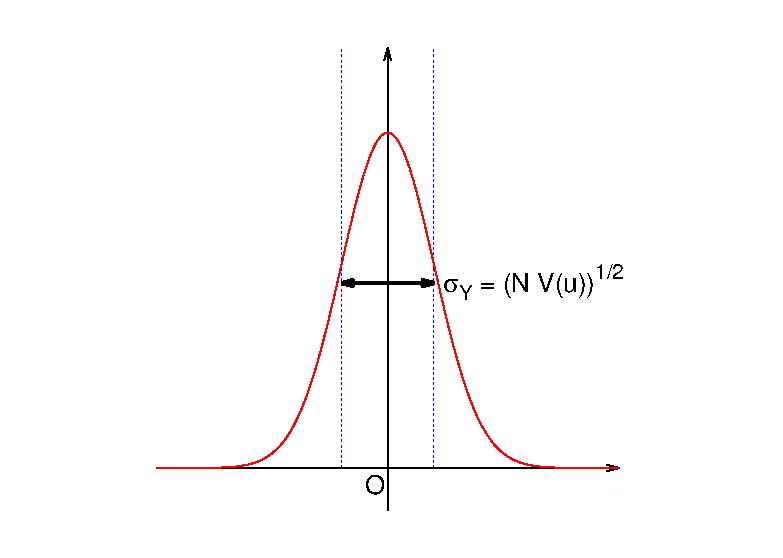
\includegraphics[width=8cm]{./figures/gauss_chain.eps}
%	\caption{末端間ベクトルの分布関数}
%\end{figure}

また、鎖の末端間ベクトルの分散 $V(\bm{R})$ は、ボンドベクトルが独立であるので、
\begin{align*}
V(\bm{R}) 
	&= V(\bm{u}_0 + \bm{u}_1 + \cdots + \bm{u}_{N-1}) \\
	&= V(\bm{u}_0) + V(\bm{u}_1) + \cdots + V(\bm{u}_{N-1}) \\
	&= N \times V(\bm{u})
\end{align*}
なお、各ボンドベクトルの長さの二乗平均を表している。

したがって、求める末端間ベクトルの確率分布関数は、
\begin{equation*}
P(\bm{R}) = \dfrac{1}{\sqrt{2 \pi N V(\bm{u})}} \exp \left(-\dfrac{\bm{R}^2}{2 N V(\bm{u})} \right)
\end{equation*}
というガウス分布に従うことになる。



\newpage

\subsubsection{フーリエ変換を用いた末端間ベクトルの確率分布の計算}

\begin{boxnote}
前問では末端間ベクトルを中心極限定理を用いて計算しましたが、ここではフーリエ変換を用いて計算してみます。

\end{boxnote}

\vspace{10pt}

\begin{enumerate}
\setlength{\parskip}{0cm} % 段落間
\setlength{\itemsep}{0.5cm} % 項目間

\item
$N+1$ 個のビーズからなる高分子鎖の格子モデルにおいて、末端間ベクトル $\bm{R}$ の確率分布関数 $P(\bm{R})$ をそれぞれのボンドベクトルの同時分布関数 $P_N(\{\bm{u}_i\})$ を用いて表したとき、末端間ベクトル分布関数 $P(\bm{R})$ が以下のように逆フーリエ変換の形で表せることを示せ
\footnote
{
フーリエ変換については、
\href{https://dl.dropboxusercontent.com/u/18899343/Math/Fourier_Transform_2014_0321.pdf}{「フーリエ変換について」}
を参照していただきたい。
}。
\begin{align*}
P(\bm{R}) 
	&= \dfrac{1}{(2 \pi)^3} \int \diff \bm{q} \exp \left( -i \bm{q} \cdot \bm{R} \right) \left[\tilde{P}_1 (\bm{q}) \right]^N \\
\end{align*}
なお、チルダのついた $\tilde{P}_1 (\bm{q})$ はフーリエ変換された量であることを表している。

\begin{itembox}[l]{{\bf ヒント:}}

互いに独立な複数の確率変数 $X_1, X_2, \cdots$ があるときに、これらの確率変数の和 $Y=X_1 + X_2 + \cdots$ も確率変数になるが、この $Y$ の確率分布は以下となる。
\begin{equation*}
P_Y(y) = \int \diff x_1 \int \diff x_2 \cdots \delta (x_1 + x_2 + \cdots -y) P_X(x_1) P_X(x_2) \cdots
\end{equation*}
\end{itembox}

\item
$N$ が大きいとき鎖の長距離での性質が重要となり、これは、波数ベクトル $|\bm{q}|$ が小さい領域に相当する。
この考えに立ち、以下の $P_1 (\bm{u})$ からのフーリエ変換において、
\begin{align*}
\tilde{P}_1 (\bm{q}) 
	&= \int \diff \bm{u} \exp(- i\bm{q} \cdot \bm{u} ) P_1 (\bm{u})
\end{align*}
指数関数の部分を波数に関してテイラー展開し、波数空間で以下のガウス分布となることを示せ。
\begin{align*}
\tilde{P}_1 (\bm{q}) 
	&\sim \exp \left( - \dfrac{a^2}{6} |\bm{q}|^2 \right)
\end{align*}

\begin{itembox}[l]{{\bf ヒント:}}

波数ベクトル空間は三次元だが、実空間での一次元の場合と同じようにテイラー展開することが可能であり、表式は以下となる。
\begin{align*}
\exp(- i\bm{q} \cdot \bm{u} )
	&\simeq \left \{ 1-( i \bm{q} \cdot \bm{u} ) +\dfrac{1}{2} (-i \bm{q} \cdot \bm{u})^2 + \cdots \right\} 
\end{align*}

また、ベクトルの内積をとった項の二乗は、ダイアディック積を用いて以下の様に書き換えることができる。
\begin{align*}
(\bm{q} \cdot \bm{u})^2 = \bm{q} \cdot (\bm{u} \bm{u}) \cdot \bm{q}
\end{align*}
\color{black}
\end{itembox}

\item
上記の結果を当初の逆フーリエ変換の式に代入し、末端間ベクトルの分布関数 $P(\bm{R})$ を実空間で求め、ガウス分布となることを示せ。
\begin{align*}
P(\bm{R}) 
	&= \left( \dfrac{3}{2 \pi N a^2} \right)^{3/2} \exp \left( -\dfrac{3|\bm{R}|^2}{2Na^2} \right)
\end{align*}



\begin{itembox}[l]{{\bf ヒント:}}
波数空間におけるガウス分布を逆フーリエ変換する計算である。
具体的な解き方としては、「微分方程式による解法」と「複素関数の性質を利用した解法」が知られている。
\end{itembox}


\item
上記の分布関数から二乗平均末端間距離を算出し、この結果が意味することを説明せよ。

\vspace{10pt}

\begin{itembox}[l]{{\bf ヒント:}}

二乗平均末端間距離は、以下のように求めることができる。

\begin{align*}
\langle |\bm{R}|^2 \rangle 
	&= \int |\bm{R}|^2 P(\bm{R}) \diff \bm{R} 
\end{align*}

この導出の際に使用するガウス積分の公式は、
\begin{align*}
\int_{-\infty}^{\infty} x^2n \exp(-ax^2) \diff x = \dfrac{(2n-1)!! \sqrt{\pi}}{2^n} \left( \dfrac{1}{a} \right)^{{2n+1}/{2}}\quad \text{ただし、$n$ は正の整数。}
\end{align*}


なお、式中にある $!!$ は二重階乗であり、 自然数 $n$ に対し、$n$ が奇数なら 1 から $n$ までの奇数の総乗、$n$ が偶数なら 2 から $n$ までの偶数の総乗である。
要するに、一つとびで掛け合わせる階乗のことであり、$0!! = 1$ である。

\end{itembox}


\end{enumerate}

\newpage 

\begin{enumerate}
\item
$N+1$ 個のビーズからなる高分子鎖の格子モデルにおいて、末端間ベクトル $\bm{R}$ の確率分布関数 $P(\bm{R})$ をそれぞれのボンドベクトルの同時分布関数 $P_N(\{\bm{u}_i\})$ を用いて表したとき、末端間ベクトル分布関数 $P(\bm{R})$ が以下のように逆フーリエ変換の形で表せることを示せ
\footnote
{
フーリエ変換については、
\href{https://dl.dropboxusercontent.com/u/18899343/Math/Fourier_Transform_2014_0321.pdf}{「フーリエ変換について」}
を参照していただきたい。
}。
\begin{align*}
P(\bm{R}) 
	&= \dfrac{1}{(2 \pi)^3} \int \diff \bm{q} \exp \left( -i \bm{q} \cdot \bm{R} \right) \left[\tilde{P}_1 (\bm{q}) \right]^N \\
\end{align*}
なお、チルダのついた $\tilde{P}_1 (\bm{q})$ はフーリエ変換された量であることを表している。

%\vspace{10pt}

\begin{itembox}[l]{{\bf ヒント:}}

互いに独立な複数の確率変数 $X_1, X_2, \cdots$ があるときに、これらの確率変数の和 $Y=X_1 + X_2 + \cdots$ も確率変数になるが、この $Y$ の確率分布は以下となる。
\begin{equation*}
P_Y(y) = \int \diff x_1 \int \diff x_2 \cdots \delta (x_1 + x_2 + \cdots -y) P_X(x_1) P_X(x_2) \cdots
\end{equation*}
\end{itembox}

\vspace{10pt}
{\bf (解答例)}

$N+1$ 個のビーズからなる理想鎖の $N$ 個の独立なボンドベクトルの同時分布関数 $P_N(\{\bm{u}_i\})$ は、$1$ 個のボンドベクトルの分布関数である $P_1$ により、以下のように記述される。
\begin{align*}
P_N(\{\bm{u}_i\}) 
	&\equiv P_N(\bm{u}_0, \bm{u}_1, \cdots, \bm{u}_{N-1})\\
	&= P_1(\bm{u}_0) P_1(\bm{u}_1) \cdots P_1(\bm{u}_{N-1})
\end{align*}

このとき、末端間ベクトルが $\bm{R}$ となる確率 $P(\bm{R})$ は、上記の同時分布関数 $P_N(\{\bm{u}_i\}) $ をデルタ関数 $\delta \left( \sum_{i=0}^{N-1} \bm{u}_i - \bm{R} \right)$ とともに用いて、以下のように表すことができる。
\begin{align*}
P(\bm{R}) 
	&\equiv \int \diff \bm{u}_0 \cdots \int \diff \bm{u}_{N-1} \delta \left( \sum_{i=0}^{N-1} \bm{u}_i - \bm{R} \right) P_N(\{\bm{u}_i \}) \\
	&= \dfrac{1}{(2 \pi)^3} \int \diff \bm{u}_0 \cdots \int \diff \bm{u}_{N-1} \int \diff \bm{q} \exp \left[ i \bm{q} \cdot \left( \sum_{i=0}^{N-1} \bm{u}_i - \bm{R} \right) \right] \prod_{j=0}^{N-1} P_1 (\bm{u}_j) \\
	&= \dfrac{1}{(2 \pi)^3} \int \diff \bm{q} \exp \left( -i \bm{q} \cdot \bm{R} \right) \prod_{j=0}^{N-1} \int \diff \bm{u}_j \exp(i\bm{q} \cdot \bm{u}_j ) P_1 (\bm{u}_j) \\
	&= \dfrac{1}{(2 \pi)^3} \int \diff \bm{q} \exp \left( -i \bm{q} \cdot \bm{R} \right) \left[\tilde{P}_1 (\bm{q}) \right]^N \\
\end{align*}
なお、チルダのついた $\tilde{P}_1 (\bm{q})$ はフーリエ変換された量であることを表しており、最後の行はその逆フーリエ変換となっている。
\newpage


\item
$N$ が大きいとき鎖の長距離での性質が重要となり、これは、波数ベクトル $|\bm{q}|$ が小さい領域に相当する。
この考えに立ち、以下の $P_1 (\bm{u})$ からのフーリエ変換において、
\begin{align*}
\tilde{P}_1 (\bm{q}) 
	&= \int \diff \bm{u} \exp(- i\bm{q} \cdot \bm{u} ) P_1 (\bm{u})
\end{align*}
指数関数の部分を波数に関してテイラー展開し、波数空間で以下のガウス分布となることを示せ。
\begin{align*}
\tilde{P}_1 (\bm{q}) 
	&\sim \exp \left( - \dfrac{a^2}{6} |\bm{q}|^2 \right)
\end{align*}

%\vspace{10pt}


%\color{red}

\begin{itembox}[l]{{\bf ヒント:}}
波数ベクトル空間においても、指数関数のテイラー展開は一変数の場合と同様に以下となる。
\begin{align*}
\exp(- i\bm{q} \cdot \bm{u} )
	&\simeq \left \{ 1-( i \bm{q} \cdot \bm{u} ) +\dfrac{1}{2} (-i \bm{q} \cdot \bm{u})^2 + \cdots \right\} 
\end{align*}

また、ベクトルの内積をとった項の二乗は、ダイアディック積により展開される。
\begin{align*}
(\bm{q} \cdot \bm{u})^2 = \bm{q}^{T} \cdot (\bm{u} \bm{u}) \cdot \bm{q}
\end{align*}

\end{itembox}

\vspace{10pt}

{\bf (解答例)}

波数ベクトルが小さい領域において、上式の指数関数の部分を波数ベクトル $\bm{q}$ に関してテイラー展開することが妥当となるので、
\begin{align*}
\tilde{P}_1 (\bm{q}) 
	&= \int \diff \bm{u} \exp(- i\bm{q} \cdot \bm{u} ) P_1 (\bm{u}) \\
	&\simeq \int \diff \bm{u} P_1 (\bm{u}) \left \{ 1-( i \bm{q} \cdot \bm{u} ) +\dfrac{1}{2} (-i \bm{q} \cdot \bm{u})^2 + \cdots \right\} \\
	&= \int \diff \bm{u} P_1 (\bm{u}) - i \int (\bm{q} \cdot \bm{u} ) P_1 (\bm{u}) d \bm{u} 
	- \dfrac{1}{2} \int (\bm{q} \cdot \bm{u})^2 P_1 (\bm{u}) d \bm{u} + \cdots \\
	&= \int \diff \bm{u} P_1 (\bm{u}) - i \bm{q} \cdot \left(\int \bm{u} P_1 (\bm{u}) d \bm{u} \right) 
	- \dfrac{1}{2} \bm{q}^{T} \cdot \left( \int (\bm{u} \bm{u}) P_1 (\bm{u}) d \bm{u} \right) \cdot \bm{q} + \cdots \\
	&= 1- i \bm{q} \cdot \langle \bm{u} \rangle 
	- \dfrac{1}{2} \bm{q}^{T} \cdot \langle \bm{u} \bm{u} \rangle \cdot \bm{q} + \cdots \\
	&= 1- i \bm{q} \cdot \bm{0} - \dfrac{1}{2} \bm{q}^{T} \cdot 
	\left (
	\begin{array}{c c c}
	\langle u_x^2 \rangle & \langle u_x u_y \rangle & \langle u_x u_z \rangle \\[10pt]
	\langle u_x u_y \rangle & \langle u_y^2 \rangle & \langle u_y u_z \rangle \\[10pt]
	\langle u_x u_z \rangle & \langle u_y u_z \rangle & \langle u_z^2 \rangle
	\end{array}
	\right)
	\cdot \bm{q} + \cdots
\end{align*}

なお、三行目の第三項での $(\bm{u} \bm{u})$ はダイアディック積である
\footnote
{
ベクトルの内積をとった項の二乗は、以下のように、ダイアディック積を用いて展開される。
\begin{align*}
(\bm{q} \cdot \bm{u})^2 = \bm{q} \cdot (\bm{u} \bm{u}) \cdot \bm{q}
\end{align*}
}。

第四行目において、第一項は確率分布関数の全空間での積分であるから 1 となり、第二項および第三項からは、それぞれの因子のアンサンブル平均
\footnote
{
任意の物理量 $x$ のアンサンブル平均(期待値)は以下の式で表される。
\begin{align*}
\langle x \rangle = \int x P(x) \diff x
\end{align*}
}
が出てきている。

$\bm{u}$ はボンドベクトルであったので、そのダイアディック積はテンソルとなり
\footnote
{
ダイアッド積の定義は、以下であった。
\begin{align*}
(\bm{a} \bm{b})_{ij} \equiv a_i b_j
\end{align*}
したがって、
\begin{align*}
\bm{u} \bm{u}
=
	\left(
	\begin{array}{c c c}
	u_x^2 		& u_x u_y	& u_x u_z \\[10pt]
	u_x u_y  	& u_y^2 	& u_y u_z \\[10pt]
	u_x u_z  	& u_y u_z 	& u_z^2
	\end{array}
	\right)
\end{align*}
}、
そのアンサンブル平均は各要素のアンサンブル平均の形で、最終行の行列の形に展開できる。

ここで対象としている鎖のボンドベクトルは、ボンド長が固定($a$ としよう)で対称性を有するものを考えているので、対角項以外は 0 になる。
また、対象としている三次元の立方格子モデルにおいては、単一のボンドベクトルの確率分布関数 $P_1 (\bm{u})$ は、任意の格子点から $6$ 個の最近接格子点に向かうボンドベクトルについて等確率であるので、
\begin{align*}
&|\bm{u}|^2 = \langle u_x^2 \rangle + \langle u_x^2 \rangle + \langle u_x^2 \rangle = a^2 \\
\therefore \quad &\langle u_x^2 \rangle = \langle u_x^2 \rangle = \langle u_x^2 \rangle = \dfrac{a^2}{3}
\end{align*}

これらの関係を考慮して、$\bm{q} = (q_x, q_y, q_z)$ とすれば、
\begin{align*}
\tilde{P}_1 (\bm{q}) 
	&= 1 - \dfrac{1}{2}
	\left( 
	\begin{array}{c c c}
	q_x 	& q_y	& q_z
	\end{array}
	\right)
	\cdot 
	\left (
	\begin{array}{c c c}
	\dfrac{a^2}{3}	&	0				&	0 \\[10pt]
	0				&	\dfrac{a^2}{3}	&	0 \\[10pt]
	0				&	0				&	\dfrac{a^2}{3}
	\end{array}
	\right)
	\cdot
	\left( 
	\begin{array}{c}
	q_x \\[10pt]
	q_y \\[10pt]
	q_z
	\end{array}
	\right)
	+ \cdots \\
%
	&= 1 - \dfrac{1}{2}
	\left( 
	\begin{array}{c c c}
	q_x 	& q_y	& q_z
	\end{array}
	\right)
	\cdot
	\left( 
	\begin{array}{c}
	\dfrac{a^2}{3}q_x \\[10pt]
	\dfrac{a^2}{3}q_y \\[10pt]
	\dfrac{a^2}{3}q_z
	\end{array}
	\right)
	+ \cdots \\
%
%	&= 1 - \dfrac{a^2}{6}
%	\left( 
%	\begin{array}{c}
%	q_x^2 \\[10pt]
%	q_y^2 \\[10pt]
%	q_z^2
%	\end{array}
%	\right)
%	+ \cdots \\
%
	&= 1 - \dfrac{a^2}{6} |\bm{q}|^2 + \cdots \\
	&\simeq \exp \left( - \dfrac{a^2}{6} |\bm{q}|^2 \right)
\end{align*}


結局、求める分布関数のフーリエ変換である $\tilde{P}_1 (\bm{q}) $ は、波数空間におけるガウス分布の形をしていることになる。

\newpage

\color{black}

\item
上記の結果を当初の逆フーリエ変換の式に代入し、末端間ベクトルの分布関数 $P(\bm{R})$ を実空間で求め、ガウス分布となることを示せ。
\begin{align*}
P(\bm{R}) 
	&= \left( \dfrac{3}{2 \pi N a^2} \right)^{3/2} \exp \left( -\dfrac{3|\bm{R}|^2}{2Na^2} \right)
\end{align*}

%\vspace{10pt}

\begin{itembox}[l]{{\bf ヒント:}}
波数空間におけるガウス分布を逆フーリエ変換する計算である。
具体的な解き方としては、「微分方程式による解法」と「複素関数の性質を利用した解法」が知られている。
\end{itembox}

{\bf 解答例 1: 微分方程式を用いた式展開}


求める分布関数のフーリエ変換である $\tilde{P}_1 (\bm{q}) $ を当初の式に代入する。
\begin{align*}
P(\bm{R}) 
	&= \dfrac{1}{(2 \pi)^3} \int \diff \bm{q} \exp \left( -i \bm{q} \cdot \bm{R} \right) \left[\tilde{P}_1 (\bm{q}) \right]^N \\
	&\sim \dfrac{1}{(2 \pi)^3} \int \diff \bm{q} \exp \left( -i \bm{q} \cdot \bm{R} \right) \exp \left( - \dfrac{Na^2}{6} |\bm{q}|^2 \right)
\end{align*}

両辺を $\bm{R}$ で微分して、
\begin{align*}
\dfrac{ \diff P(\bm{R})}{\diff \bm{R}} 
	&=\dfrac{1}{(2 \pi)^3} \difd{}{\bm{R}} \left[ \int \diff \bm{q} \exp \left( -i \bm{q} \cdot \bm{R} \right) \exp \left( - \dfrac{Na^2}{6} |\bm{q}|^2 \right) \right] \\
	&=\dfrac{1}{(2 \pi)^3} \int \exp \left( - \dfrac{Na^2}{6} |\bm{q}|^2 \right) \difp{}{\bm{R}} \exp \left( -i \bm{q} \cdot \bm{R} \right) \diff \bm{q} \\
	&= -i \dfrac{1}{(2 \pi)^3} \int \bm{q} \exp \left( - \dfrac{Na^2}{6} |\bm{q}|^2 \right) \exp \left( -i \bm{q} \cdot \bm{R} \right) \diff \bm{q}
\end{align*}

ここで、
\begin{align*}
&\dfrac{ \diff}{\diff \bm{q}} \exp \left( - \dfrac{Na^2}{6} |\bm{q}|^2 \right) = 2\times \left( -\dfrac{Na^2}{6} \right)  \bm{q} \exp \left(- \dfrac{Na^2}{6} |\bm{q}|^2 \right) \\
\therefore \quad &\bm{q} \exp \left( - \dfrac{Na^2}{6} |\bm{q}|^2 \right) = - \dfrac{3}{Na^2} \dfrac{ \diff}{\diff \bm{q}} \exp \left( - \dfrac{Na^2}{6} |\bm{q}|^2 \right) 
\end{align*}
と変形できるので、これを、先ほどの式に代入して部分積分の公式を使うと、
\begin{align*}
\dfrac{ \diff P(\bm{R})}{\diff \bm{R}} 
	&= i \dfrac{3}{Na^2} \left( \dfrac{1}{2 \pi} \right)^3 \int \dfrac{ \diff}{\diff \bm{q}} \exp \left( - \dfrac{Na^2}{6} |\bm{q}|^2 \right) \exp \left( -i \bm{q} \cdot \bm{R} \right) \diff \bm{q}\\
	&= i \dfrac{3}{Na^2} \left( \dfrac{1}{2 \pi} \right)^3 \left\{ \left[\exp \left( - \dfrac{Na^2}{6} |\bm{q}|^2 \right) \exp \left( -i \bm{q} \cdot \bm{R} \right) \right]_{-\infty}^{\infty} \right. \\
	&\quad \left. + i \bm{R} \int \exp \left( - \dfrac{Na^2}{6} |\bm{q}|^2 \right) \exp \left( -i \bm{q} \cdot \bm{R} \right) \diff \bm{q} \right\} \\
	&= - \dfrac{3 \bm{R} }{Na^2} \left( \dfrac{1}{2 \pi} \right)^3 \int \exp \left( - \dfrac{Na^2}{6} |\bm{q}|^2 \right) \exp \left( -i \bm{q} \cdot \bm{R} \right) \diff \bm{q} \\
	&= - \dfrac{3 \bm{R} }{Na^2} P(\bm{R})
\end{align*}

なお、二行目の第一項の定積分は、$N>0$ なので、$\bm{q} \rightarrow \pm \infty$ のときに $\exp \left(- \dfrac{Na^2}{6} |\bm{q}|^2 \right) \rightarrow 0 $ であるから $0$ となる。

続いて、上述のように得た微分方程式を展開しよう。
\begin{align*}
\dfrac{ \diff P(\bm{R})}{\diff \bm{R}} &= - \dfrac{3 \bm{R} }{Na^2} P(\bm{R}) \\
\int \dfrac{1}{P(\bm{R})} \diff P(\bm{R}) &= - \dfrac{3}{Na^2} \int \bm{R} \diff \bm{R} \\
\ln P(\bm{R}) &= - \dfrac{3}{Na^2} \dfrac{|\bm{R}|^2}{2} + C \\
\therefore \quad P(\bm{R}) &= C \exp \left( - \dfrac{3|\bm{R}|^2}{2 Na^2} \right)
\end{align*}

積分定数 $C$ は、上式に $\bm{R}=\bm{0}$ を代入して、
\begin{align*}
P(\bm{R}=\bm{0}) = C
\end{align*}

一方、当初の逆フーリエ変換のガウス積分より、
\begin{align*}
P(\bm{R}=\bm{0}) 
	&= \dfrac{1}{(2 \pi)^3} \int \diff \bm{q} \exp \left( - \dfrac{Na^2}{6} |\bm{q}|^2 \right) \\
	&= \dfrac{1}{(2 \pi)^3} \sqrt{\left( \dfrac{6 \pi}{N a^2} \right)^{3} }\\
	&= \left( \dfrac{6 \pi}{(2 \pi)^2 N a^2} \right)^{3/2} \\
	&= \left( \dfrac{3}{2 \pi N a^2} \right)^{3/2} = C
\end{align*}

したがって、求める分布関数として、
\begin{align*}
P(\bm{R}) 
	&\sim \left( \dfrac{3}{2 \pi N a^2} \right)^{3/2} \exp \left( -\dfrac{3|\bm{R}|^2}{2Na^2} \right)
\end{align*}
のように、末端間ベクトルについてのガウス分布を得る。

\newpage

\vspace{10pt}

{\bf 解答例 2: 複素関数の性質を利用した式展開}

求める分布関数のフーリエ変換である $\tilde{P}_1 (\bm{q}) $ を当初の式に代入し、平方完成により、
\begin{align*}
P(\bm{R}) 
	&= \dfrac{1}{(2 \pi)^3} \int \diff \bm{q} \exp \left( -i \bm{q} \cdot \bm{R} \right) \left[\tilde{P}_1 (\bm{q}) \right]^N \\
	&\sim \dfrac{1}{(2 \pi)^3} \int \diff \bm{q} \exp \left( -i \bm{q} \cdot \bm{R} \right) \exp \left( - \dfrac{Na^2}{6} |\bm{q}|^2 \right) \\
	&= \dfrac{1}{(2 \pi)^3} \int \diff \bm{q} \exp \left[ - \dfrac{Na^2}{6} \left( |\bm{q}|^2 + i \dfrac{6}{Na^2}\bm{q} \cdot \bm{R} \right) \right] \\
	&= \dfrac{1}{(2 \pi)^3} \int \diff \bm{q} \exp \left[ - \dfrac{Na^2}{6} \left\{ \left( |\bm{q}| + i \dfrac{3}{Na^2} \bm{R} \right)^2 - \left( i \dfrac{3}{Na^2} \bm{R} \right)^2 \right\} \right] \\
	&= \dfrac{1}{(2 \pi)^3} \int \diff \bm{q} \exp \left[ - \dfrac{Na^2}{6} \left( |\bm{q}| + i \dfrac{3}{Na^2} \bm{R} \right)^2 - \dfrac{3}{2Na^2} |\bm{R}|^2  \right] \\
	&= \exp \left(- \dfrac{3}{2Na^2} |\bm{R}|^2  \right) \times \dfrac{1}{(2 \pi)^3} \int \diff \bm{q} \exp \left[ - \dfrac{Na^2}{6} \left( |\bm{q}| + i \dfrac{3}{Na^2} \bm{R} \right)^2 \right]
\end{align*}
となる
\footnote{
この方法についての詳細は、\href{https://dl.dropboxusercontent.com/u/18899343/Math/Fourier_Transform.pdf}{「フーリエ変換について」}を参照していただきたい。
}。

複素関数の性質を利用することにより、上式の $\exp$ 以降の因子は、
\begin{align*}
\dfrac{1}{(2 \pi)^3} \int \diff \bm{q} \exp \left[ - \dfrac{Na^2}{6} \left( |\bm{q}| + i \dfrac{3}{Na^2} \bm{R} \right)^2 \right] 
	&= \dfrac{1}{(2 \pi)^3} \int \diff \bm{x} \exp \left[ - \dfrac{Na^2}{6} \bm{x}^2 \right] \\
	&= \dfrac{1}{(2 \pi)^3} \sqrt{\left( \dfrac{\pi}{\dfrac{N a^2}{6}} \right)^{3} }\\
	&= \left( \dfrac{6 \pi}{(2 \pi)^2 N a^2} \right)^{3/2} \\
	&= \left( \dfrac{3}{2 \pi N a^2} \right)^{3/2} \\
\end{align*}

したがって、求める分布関数として、
\begin{align*}
P(\bm{R}) 
	&\sim \left( \dfrac{3}{2 \pi N a^2} \right)^{3/2} \exp \left( -\dfrac{3|\bm{R}|^2}{2Na^2} \right)
\end{align*}
のように、末端間ベクトルについてのガウス分布を得る。

\newpage

\item
上記の分布関数から二乗平均末端間距離を算出し、この結果が意味することを説明せよ。

\vspace{10pt}

\begin{itembox}[l]{{\bf ヒント:}}

二乗平均末端間距離は、以下のように求めることができる。

\begin{align*}
\langle |\bm{R}|^2 \rangle 
	&= \int |\bm{R}|^2 P(\bm{R}) \diff \bm{R} 
\end{align*}

この導出の際に使用するガウス積分の公式は、
\begin{align*}
\int_{-\infty}^{\infty} x^2n \exp(-ax^2) \diff x = \dfrac{(2n-1)!! \sqrt{\pi}}{2^n} \left( \dfrac{1}{a} \right)^{{2n+1}/{2}}\quad \text{ただし、$n$ は正の整数。}
\end{align*}
なお、式中にある $!!$ は二重階乗であり、 自然数 $n$ に対し、$n$ が奇数なら 1 から $n$ までの奇数の総乗、$n$ が偶数なら 2 から $n$ までの偶数の総乗である。
要するに、一つとびで掛け合わせる階乗のことであり、$0!! = 1$ である。

\color{black}
\end{itembox}

\vspace{10pt}

{\bf (解答例)}

これまでに求めた末端間距離の確率分布関数 $P(\bm{R}) $ を用いて、末端間距離二乗平均 $\langle |\bm{R}|^2 \rangle$ を求めてみよう。
\begin{align*}
\langle |\bm{R}|^2 \rangle 
	&= \int |\bm{R}|^2 P(\bm{R}) \diff \bm{R} \\ 
	&= \int |\bm{R}|^2 \left( \dfrac{3}{2 \pi N a^2} \right)^{3/2} 
		\exp \left( -\dfrac{3|\bm{R}|^2}{2 N a^2} \right) \diff \bm{R} \\
	&= \left( \dfrac{3}{2 \pi N a^2} \right)^{3/2} \int |\bm{R}|^2  
		\exp \left( -\dfrac{3|\bm{R}|^2}{2 N a^2} \right) \diff \bm{R} \\
	&= \left( \dfrac{3}{2 \pi N a^2} \right)^{3/2} 
		\int_0^{\infty} \int_0^{\pi} \int_0^{2 \pi}
		r^2 \exp \left( -\dfrac{3 r^2}{2 N a^2} \right) r^2 \sin \theta \diff r \diff \theta \diff \varphi \\
	&= \left( \dfrac{3}{2 \pi N a^2} \right)^{3/2} 
		\int_0^{\infty}
		r^4 \exp \left( -\dfrac{3 r^2}{2 N a^2} \right) \diff r \int_0^{\pi} \sin \theta \diff \theta \int_0^{2 \pi} \diff \varphi \\
	&= \left( \dfrac{3}{2 \pi N a^2} \right)^{3/2} \dfrac{3 \sqrt{\pi}}{4} \left(\dfrac{2 N a^2}{3} \right)^{5/2} \times 1 \times 2\pi \\
	&= N a^2
\end{align*}
なお、四行目では極座標へと変換することでヤコビアン $r^2 \sin \theta$ がでており、六行目へは、$r$ に関する積分においてガウス積分の公式を用いた
\footnote
{
ガウス積分の公式は、
\begin{align*}
\int_{-\infty}^{\infty} x^2n \exp(-ax^2) \diff x = \dfrac{(2n-1)!! \sqrt{\pi}}{2^n} \left( \dfrac{1}{a} \right)^{{2n+1}/{2}}\quad \text{ただし、$n$ は正の整数。}
\end{align*}
なお、式中にある $!!$ は二重階乗であり、 自然数 $n$ に対し、$n$ が奇数なら 1 から $n$ までの奇数の総乗、$n$ が偶数なら 2 から $n$ までの偶数の総乗である。
}。

この確率分布関数の導出は、格子モデルに基づくボンドベクトルの性質から導出したものであり、その過程において、波数ベクトル $|\bm{q}|$ が小さい領域を対象として波数に関するテイラー展開による近似で求めたものである。
この過程においては、格子定数程度の短距離の性質を無視していることになる。
このような近似を行っているにもかかわらず、末端間距離の二乗平均に対しては、正確な値が得られる事が確認できた。

これは、独立な確率変数の多数の和が正規分布に従うという中心極限定理の帰結と考えることができる。

\end{enumerate}

\newpage

\color{black}

\subsubsection{理想鎖の慣性半径}

\begin{boxnote}
{\bf 出題意図:} 慣性半径 $R_g$ は、高分子鎖の空間的な広がりを表す指標として、実験的に求めやすいものである。
ここでは、理想鎖を対象として、その表式についての確認を行う。
%}
\end{boxnote}

\vspace{10pt}

高分子鎖の重心は、
\begin{equation*}
\bm{r}_g = \dfrac{1}{N+1} \sum_{j=0}^{N} \bm{r}_j
\end{equation*}
であり、$0 \sim N$ までの $N+1$ 個のセグメントからなる理想鎖の慣性半径 $R_g$ は、鎖の重心 $\bm{r}_g$ から各セグメントまでの距離の二乗の平均値の平方根として以下のように定義される。
\begin{equation*}
R_g^2 = \dfrac{1}{N+1} \left\langle \sum_{i=0}^{N} |\bm{r}_i - \bm{r}_g|^2 \right\rangle
\end{equation*}

$N \gg 1$ の時、
\begin{equation*}
R_g^2 \simeq \dfrac{1}{6}N a^2
\end{equation*}
となり、末端間距離と同様に鎖長 $N$ に対して $N^{1/2}$ の依存性を示すことを示せ。

\vspace{10pt}

\begin{itembox}[l]{{\bf ヒント:}}

慣性半径の定義式として、二点間の距離を用いて表したもう一つの表式がある。
\begin{equation*}
R_g^2 = \dfrac{1}{2(N+1)^2} \left \langle \sum_{i=0}^N \sum_{j=0}^N \left| \bm{r}_i - \bm{r}_j \right|^2 \right \rangle
\end{equation*}

これが、上記の確率変数の分散(あるいは二次のモーメント)を用いた定義式と等価であることを利用すればよい。
\end{itembox}

\newpage
高分子鎖の重心は、
\begin{equation*}
\bm{r}_g = \dfrac{1}{N+1} \sum_{j=0}^{N} \bm{r}_j
\end{equation*}
であり、$0 \sim N$ までの $N+1$ 個のセグメントからなる理想鎖の慣性半径 $R_g$ は、鎖の重心 $\bm{r}_g$ から各セグメントまでの距離の二乗の平均値の平方根として以下のように定義される。
\begin{equation*}
R_g^2 = \dfrac{1}{N+1} \left\langle \sum_{i=0}^{N} |\bm{r}_i - \bm{r}_g|^2 \right\rangle
\end{equation*}

$N \gg 1$ の時、
\begin{equation*}
R_g^2 \simeq \dfrac{1}{6}N a^2
\end{equation*}
となり、末端間距離と同様に鎖長 $N$ に対して $N^{1/2}$ の依存性を示すことを示せ。

\vspace{10pt}

\begin{itembox}[l]{{\bf ヒント:}}

慣性半径を表す定義式として、二点間の距離を用いて表したもう一つの表式がある。
\begin{equation*}
R_g^2 = \dfrac{1}{2(N+1)^2} \left \langle \sum_{i=0}^N \sum_{j=0}^N \left| \bm{r}_i - \bm{r}_j \right|^2 \right \rangle
\end{equation*}

これが、上記の統計的な分散(あるいはモーメント)と類似の式と等価であることを利用すればよい。
\end{itembox}

\vspace{10pt}
{\bf (解答例)}

二点間の距離により定義した表式が、一般的な重心からの距離によるものと等しいことを示そう。

アンサンブル平均の中の因子は、以下のように展開できる。
\begin{align*}
\sum_{i = 0}^N \sum_{j=0}^N \left| \bm{r}_i - \bm{r}_j \right|^2
	&= \sum_{i = 0}^N \sum_{j=0}^N  \left| (\bm{r}_i - \bm{r}_g) - (\bm{r}_j - \bm{r}_g) \right|^2 \\
	&= \sum_{i = 0}^N \sum_{j=0}^N \left[ \left| \bm{r}_i - \bm{r}_g \right|^2 + \left|\bm{r}_j - \bm{r}_g \right|^2 -2 (\bm{r}_i - \bm{r}_g) \cdot (\bm{r}_j - \bm{r}_g) \right] \\
	&= (N + 1) \left[ \sum_{i=0}^N \left| \bm{r}_i - \bm{r}_g \right|^2 + \sum_{j=0}^N \left| \bm{r}_j - \bm{r}_g \right|^2 \right] -2 \sum_{i=0}^N (\bm{r}_i - \bm{r}_g) \sum_{j=0}^N (\bm{r}_j - \bm{r}_g) \\
	&= 2(N + 1) \sum_{i=0}^N (\bm{r}_i- \bm{r}_g)^2 
\end{align*}
三行目へは、因子中に存在しないダミー変数の和が総数となり、$\sum_{i = 0}^N \sum_{j=0}^N \left| \bm{r}_i - \bm{r}_g \right|^2 = (N+1) \sum_{i = 0}^N \left| \bm{r}_i - \bm{r}_g \right|^2 $ となることを用い、さらに、最終行は、第三行第二項のそれぞれの因子が以下のように 0 となることを利用した。
\begin{align*}
\sum_{i=0}^N (\bm{r}_i - \bm{r}_g) 
	&= \sum_{i=0}^N \bm{r}_i -(N+1) \bm{r}_g \\
	&= \sum_{i=0}^N \bm{r}_i -(N+1) \dfrac{1}{N+1} \sum_{i=0}^{N} \bm{r}_i \\
	&=0
\end{align*}

これで、二点間の距離を利用して慣性半径を導出する以下の表式の妥当性が確認できた。
\begin{equation*}
R_g^2 = \dfrac{1}{2(N+1)^2} \left \langle \sum_{i=0}^N \sum_{j=0}^N \left| \bm{r}_i - \bm{r}_j \right|^2 \right \rangle
\end{equation*}

このとき、それぞれのセグメントの位置関係は、図に示したようになる。

\begin{itemize}
\item
$i < j$ の場合

\setlength\unitlength{1truecm}
\begin{picture}(12,2)(0,0)
\linethickness{0.5pt}
\put(1,1){\line(1,0){10}}
\linethickness{3pt}
\put(4,1){\line(1,0){4}}
\put(1, 1){\circle*{0.4}}
\put(4, 1){\circle*{0.4}}
%\put(6, 1){\circle*{0.4}}
\put(8, 1){\circle*{0.4}}
\put(11, 1){\circle*{0.4}}
%
\put(0.9,0.5){$0$}
\put(3.9,0.5){$i$}
%\put(5.9,0.5){$i$}
\put(7.9,0.5){$j$}
\put(10.8,0.5){$N$}
\end{picture}

ここで、考察の対象としているのは理想鎖であるから、ガウス鎖の部分鎖の統計的独立性のため、$0 \sim i$ および $j \sim N$ のセグメントをつなげた部分鎖については、隣同士のセグメントを結合するボンドのボンドベクトルのアンサンブル平均は $\bm{0}$ となる。
したがって、$i$ 番目のセグメントから、$j$ 番目のセグメントまでの部分鎖中のボンドベクトルだけを考えればよいことになる。

\item
$j < i$ の場合

\setlength\unitlength{1truecm}
\begin{picture}(12,2)(0,0)
\linethickness{0.5pt}
\put(1,1){\line(1,0){10}}
\linethickness{3pt}
\put(4,1){\line(1,0){4}}
\put(1, 1){\circle*{0.4}}
\put(4, 1){\circle*{0.4}}
%\put(6, 1){\circle*{0.4}}
\put(8, 1){\circle*{0.4}}
\put(11, 1){\circle*{0.4}}
%
\put(0.9,0.5){$0$}
\put(3.9,0.5){$j$}
%\put(5.9,0.5){$i$}
\put(7.9,0.5){$i$}
\put(10.8,0.5){$N$}
\end{picture}

$i,j$ の大小関係が反転したこちらの場合においても、条件は上記の場合とまったく同一となる。


\end{itemize}

したがって、上記二種類の等価な相関を考えればよいことになるので、例えば、 $i < j$ の場合だけを考えて 2 倍すればよい。

なお、注目する部分鎖中の任意の二つのボンドベクトルを新たなダミー変数を用いて $\bm{u}_l$ および $\bm{u}_m$ と表した場合、各ボンドの方向は無相関であるから、
\begin{align*}
\langle \bm{u}_l \cdot \bm{u}_m \rangle 
	&= \langle \bm{\hat{u}}_l \cdot \bm{\hat{u}}_m \rangle a^2 \\
	&=
\begin{cases}
\langle |\bm{\hat{u}}_l |^2 \rangle a^2 = a^2	&\quad (\text{$l = m$ のとき}) \\
\langle \bm{u}_l \rangle \cdot \langle \bm{u}_m \rangle = \bm{0}\cdot\bm{0} = 0	&\quad(\text{$l \neq m$ のとき})
\end{cases}
\end{align*}
となる。
ここで、$\bm{\hat{u}}_l \equiv \dfrac{\bm{u}_l}{|\bm{u}_l|}$ は $\bm{u}_l$ 方向の単位ベクトル、$a$ はボンドの長さを表している。
%
%したがって、求める慣性半径は、以下のように展開することができる。
%\begin{align*}
%R_g^2 
%	&= \dfrac{1}{(N+1)^3} \left \langle \sum_{i=0}^N \sum_{j=0}^{N} \sum_{k=0}^{N} (\bm{r}_i - \bm{r}_j) \cdot (\bm{r}_i - \bm{r}_k) \right \rangle \\
%	&= \dfrac{1}{(N+1)^3} \sum_{i=0}^N \sum_{k=0}^{i-1} \sum_{j=0}^{k-1} 4(i-k) \langle \bm{u}_l \cdot \bm{u}_m \rangle b_0^2 \\
%	&= \dfrac{4 a^2}{(N+1)^3} \sum_{i=0}^N \sum_{k=0}^{i-1} \sum_{j=0}^{k-1} (i-k) \\
%	&= \dfrac{4 a^2}{(N+1)^3} \sum_{i=0}^N \sum_{k=0}^{i-1} (i-k)k \\
%	&= \dfrac{4 a^2}{(N+1)^3} \sum_{i=0}^N \left [ \sum_{k=0}^{i-1} ik - \sum_{k=0}^{i-1} k^2 \right] \\
%	&= \dfrac{4 a^2}{(N+1)^3} \sum_{i=0}^N \left [ i \times \dfrac{1}{2}(i-1)i -\dfrac{1}{6}(i-1)i\{2(i-1)+1\} \right] \\
%	&= \dfrac{4 a^2}{(N+1)^3} \sum_{i=0}^N \left [ \dfrac{1}{2}(i^3 - i^2) -\dfrac{1}{6}(2i^3-3i^2+i) \right] \\
%	&= \dfrac{4 a^2}{6(N+1)^3} \sum_{i=0}^N \left ( i^3 -i \right) \\
%	&= \dfrac{4 a^2}{6(N+1)^3} \left[ \left\{\dfrac{1}{2} N (N+1) \right\}^2 -\dfrac{1}{2} N(N+1) \right] \\
%	&= \dfrac{N(N+1)\{ N(N+1) - 2 \}}{6(N+1)^3} a^2 \\
%	&= \dfrac{N(N+1)(N-1)(N+2)}{6(N+1)^3} a^2 \\
%	&\simeq \dfrac{1}{6} N a^2
%\end{align*}
%
%
%




上式の関係を利用して、結局、二つのセグメント間の距離からの慣性半径の表式を展開して、
\begin{align*}
R_g 
	&= \dfrac{1}{2(N+1)^2} \left \langle \sum_{i=0}^N \sum_{j=0}^N (\bm{r}_i - \bm{r}_j) \cdot (\bm{r}_i - \bm{r}_j) \right \rangle\\
	&= \dfrac{1}{2(N+1)^2} \left \langle 2 \sum_{i=0}^N \sum_{j=0}^{i-1} \left|\bm{r}_i - \bm{r}_j \right|^2 \right \rangle\\
	&= \dfrac{a^2}{(N+1)^2} \sum_{i=0}^N \sum_{j=0}^{i-1} (i -j) \\
	&= \dfrac{a^2}{(N+1)^2} \sum_{i=0}^N \left \{i^2 - \left (\dfrac{1}{2} \left (i-1 \right ) i \right) \right\} \\
	&= \dfrac{a^2}{2(N+1)^2} \sum_{i=0}^N (i^2 + i) \\
	&= \dfrac{a^2}{2(N+1)^2} \left\{ \dfrac{1}{6} N (N+1)(2N+1) + \left (\dfrac{1}{2} N (N + 1) \right) \right\} \\
	&= \dfrac{a^2}{12(N+1)^2} ( 2N^3  + 3N^2 + N + 3N^2 + 3N ) \\
	&= \dfrac{N(N+1)(N+2) }{6(N+1)^2} a^2\\
	&\sim \dfrac{N}{6} a^2\\
\end{align*}
二行目へは $i < j$ の場合だけを対象として、因子を二倍している。
また、四および六行目では、累乗の和に関する公式を用いた
\footnote{
累乗の和に関する公式は、以下のようになっている。
\begin{equation*}
\begin{cases}
\displaystyle \sum_{i=0}^{N} i = \dfrac{1}{2} N (N+1) \\[12pt]
\displaystyle \sum_{i=0}^{N} i^2 = \dfrac{1}{6} N (N+1)(2N+1) \\[12pt]
\displaystyle \sum_{i=0}^{N} i^3 = \left\{\dfrac{1}{2} N (N+1) \right\}^2
\end{cases}
\end{equation*}
}。
なお、四行目では初項 $0$、末項 $i-1$ として公式を用いている。 

%\vspace{10pt}

\newpage
{\bf (おまけ:積分形式での解)}

上式は、離散的な和の形で表して公式を利用して解いているが、一般的に積分の形で書くと以下のようになる。

なお、こちらの展開においては、上記の展開で行った $i , j$ の大小関係に基づく絶対値の場合分けを積分範囲の分割という形で行っているので、式中には 2 の因子はでてこない。
\begin{align*}
R_g 
	&= \dfrac{1}{2(N+1)^2} \left \langle \int_{0}^N \diff i \int_{0}^N \diff j (\bm{r}_i - \bm{r}_j) \cdot (\bm{r}_i - \bm{r}_j) \right \rangle\\
	&= \dfrac{1}{2(N+1)^2} \left \langle \int_{0}^N \diff i \int_{0}^{N} \diff j \left|\bm{r}_i - \bm{r}_j \right|^2 \right \rangle\\
	&= \dfrac{a^2}{2(N+1)^2} \int_{0}^N \diff i \int_{0}^{N} \diff j \left|\bm{r}_i - \bm{r}_j \right| \\
	&= \dfrac{a^2}{2(N+1)^2} \int_{0}^N \diff i \left\{ \int_{0}^{i} \diff j (i -j) + \int_i^N \diff j \left[ -(i-j) \right] \right\} \\
	&= \dfrac{a^2}{2(N+1)^2} \int_{0}^N \diff i \left\{ \left [ij - \dfrac{j^2}{2} \right]_0^i - \left[ ij - \dfrac{j^2}{2} \right]_i^N \right\} \\
	&= \dfrac{a^2}{2(N+1)^2} \int_{0}^N \diff i \left\{ \left (i^2 - \dfrac{i^2}{2} \right) - \left[ \left(Ni - \dfrac{N^2}{2} \right) - \left (i^2 - \dfrac{i^2}{2} \right) \right] \right\} \\
	&= \dfrac{a^2}{2(N+1)^2} \int_{0}^N \diff i \left\{ i^2 - Ni + \dfrac{N^2}{2} \right\} \\
	&= \dfrac{a^2}{2(N+1)^2} \left[ \dfrac{i^3}{3} - \dfrac{N}{2}i^2 + \dfrac{N^2}{2} i \right]_0^N \\
	&= \dfrac{a^2}{2(N+1)^2} \left( \dfrac{N^3}{3} - \dfrac{N^3}{2} + \dfrac{N^3}{2} \right) \\
	&= \dfrac{N^3 }{6(N+1)^2} a^2\\
	&\sim \dfrac{N}{6} a^2\\
\end{align*}

\color{black}

\newpage

\subsection{相分離}

\subsubsection{一様混合状態の安定限界}

\begin{boxnote}
熱力学ポテンシャルによる系の安定性条件を用いて、二成分混合系の一様状態の安定限界(スピノダル)を定義し、二成分系の相図を計算する手法を学ぶ問題です。

\end{boxnote}

\vspace{10pt}

\begin{enumerate}
\setlength{\parskip}{0cm} % 段落間
\setlength{\itemsep}{0.5cm} % 項目間

\item
ある平衡系の熱力学的状態が変数 $\phi$ で表されるものとする。
(例としては、$\phi$ は粒子密度など。) 
この系の一様状態の自由エネルギーを $F(\phi)$ とする。
この一様状態が熱力学的に不安定になる条件を求めよ。
($\phi$ が濃度の場合、この安定限界をスピノダルと呼ぶ。)

\begin{itembox}[l]{{\bf ヒント:}}
自由エネルギー曲線の形状と濃度ゆらぎとの関係について考察し、不安定条件を定めよ。
\end{itembox}

\item
二つの相が共存する条件を示せ。
なお、自由エネルギーを用いて表わすこととする。

\begin{itembox}[l]{{\bf ヒント:}}
粒子数と共役な変数について考察を進め、二相が共存する条件を自由エネルギー曲線で表すことを考えよ。
\end{itembox}

\end{enumerate}


\newpage







\begin{enumerate}
\setlength{\parskip}{0cm} % 段落間
\setlength{\itemsep}{0.5cm} % 項目間

\color{black}
\vspace{10pt}
\item
ある平衡系の熱力学的状態が変数 $\phi$ で表されるものとする。
(例としては、$\phi$ は粒子密度など。) 

この系の一様状態の自由エネルギーを $F(\phi)$ とする。
この一様状態が熱力学的に不安定になる条件を求めよ。
($\phi$ が濃度の場合、この安定限界をスピノダルと呼ぶ。)

\begin{itembox}[l]{{\bf ヒント:}}
自由エネルギー曲線の形状と濃度ゆらぎとの関係について考察し、不安定条件を定めよ。
\end{itembox}

\vspace{10pt}
{\bf (解答例
\footnote
{
ここで行った議論に関しては、
\href{https://dl.dropboxusercontent.com/u/18899343/physics/FreeEnergyForm/Free_Energy_Form.pdf}{「混合系の相分離条件」}
を参照していただきたい。
}
)}

ここでは、系の任意の状態を表す変数 $\phi$ を体積分率とする。
単位体積当たりの自由エネルギーである自由エネルギー密度を、系の一様混合状態における自由エネルギー $F(\phi)$ を系の体積 $V$ で除した $f (\phi)= \dfrac{F(\phi)}{V}$ で表すと、系の局所的な状態の評価に便利である。

自由エネルギー密度 $f(\phi)$ は、A成分の体積分率 $\phi$ により定まる $(\phi, f(\phi) )$ 平面上の曲線として表され、局所的な状態は、局所的なA成分の体積分率により定まる局所的な自由エネルギー密度 $f_{local}$ により評価できる。
したがって、一様状態の系全体の状態を表す $f(\phi)$ と局所的な状態の $f_{local}$ との大小関係から、局所的な濃度ゆらぎの安定性を評価できることになる。

ここで、具体的に、局所的に濃度ゆらぎが生じて A 成分が基準状態である $\phi$ から $\phi_{\alpha}$ と $\phi_{\beta}$ との二つの状態にゆらいだ場合を考えよう。
\begin{figure}[htbp]
	\centering
		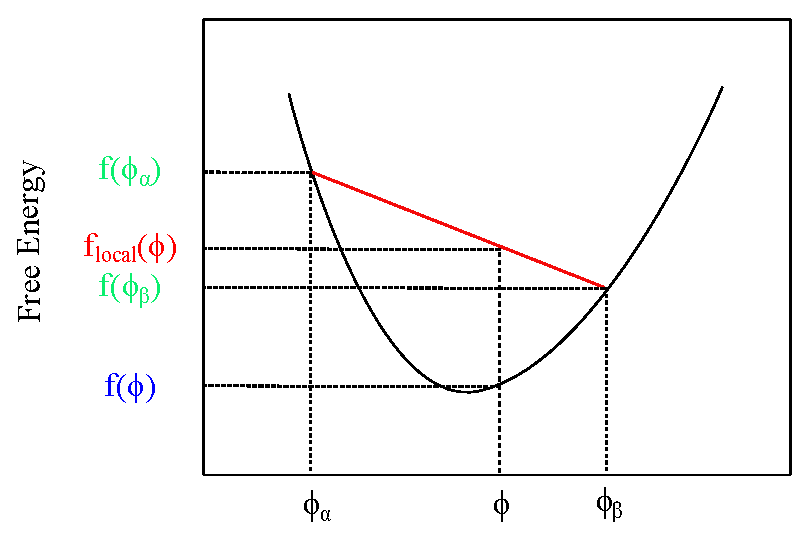
\includegraphics[width = 8 cm]{./figures/fig2.eps}
	\caption{自由エネルギー曲線が下に凸}
\end{figure}

それぞれの状態の局所的な体積を $v_{\alpha}, v_{\beta}$ とすれば
\footnote
{
本来、局所的なゆらぎの範囲を限定することは困難であり、$v_{\alpha}, v_{\beta}$ の値は不定であるが、ここでは単純化して局所的な場の元々の体積を $v$ で、$v= v_{\alpha} + v_{\beta}$ とする。
}、
局所的な自由エネルギー密度 $f_{local}(\phi)$ は、以下のように近似できる。
\begin{align*}
f_{local}(\phi)
	&= \dfrac{v_{\alpha} f(\phi_{\alpha}) + v_{\beta} f(\phi_{\beta})}{v_{\alpha} + v_{\beta}} \\
	&= \dfrac{f (\phi_\alpha) -f (\phi_\beta)}{\phi _\alpha -\phi _\beta} (\phi - \phi _\beta) + f (\phi_\beta)
\end{align*}
なお、二行目へは、成分 $A$ の物質収支に着目して変形した
\footnote
{
非圧縮性より、
\begin{align*}
	& \phi v = \phi_\alpha v_\alpha + \phi_\beta (v - v_\alpha) \\
	& v_\alpha (\phi_\beta - \phi_\alpha) = v(\phi_\beta - \phi) 
\end{align*}
}。


この場合の局所的な自由エネルギー密度 $f_{local} (\phi)$ は、 $(\phi, f(\phi) )$ 平面において、「必ず」二点、$(\phi_\alpha, f (\phi_\alpha) )$ と $(\phi_\beta, f (\phi_\beta) )$ とを結ぶ直線上にあり、体積分率が基準状態である $\phi$ である点 $(\phi, f_{local}(\phi) )$ となる。

系が一様状態を維持するためには、この状態変数の変動に対して $f_{local} (\phi)$ が減少しないこと、すなわち、$f_{local} (\phi) \geq f(\bar{\phi})$ が要請される。
これは、$\phi$ の近傍において、自由エネルギー曲線が下に凸となっていることに対応する。
自由エネルギー曲線がこのような形状となっていれば、上記条件を満たし状態変数のゆらぎが抑制されることになる。

\begin{figure}[htbp]
	\centering
		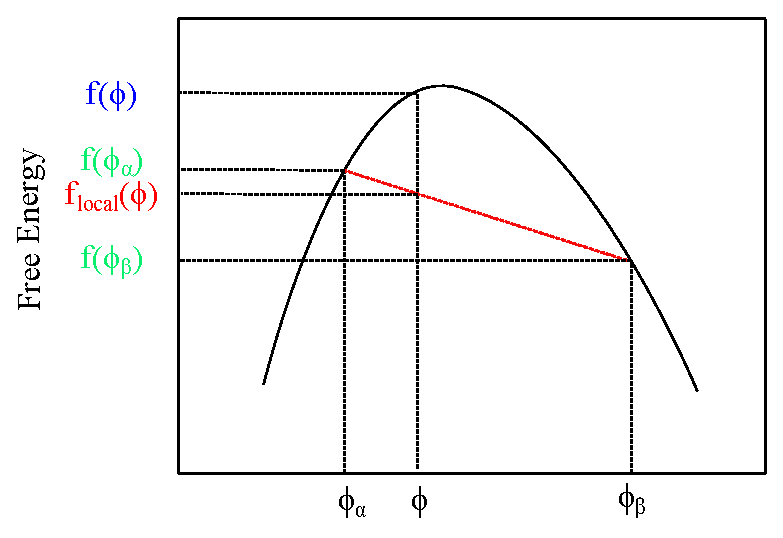
\includegraphics[width = 8 cm]{./figures/fig3.eps}
	\caption{自由エネルギー曲線が上に凸}
\end{figure}

逆に考えた場合、系が熱力学的に不安定となる条件とは、状態変数が揺らいだ時に、そのゆらぎに応じて系の局所的な自由エネルギー $f_{local} (\phi)$ が減少してしまうことに対応する。
すなわち、状態変数のゆらぎに伴って系の自由エネルギーが局所的に減少すれば、系はゆらぎに基づく二つの状態へと分離することになり、その状態での新たな状態変数に応じてさらに系全体が変化していくことになる。

したがって、系が不安定となる条件とは、自由エネルギー曲線中に上に凸な範囲が生じることとなる。
\vspace{10pt}

\color{black}

\newpage

\item
2 つの相が共存する条件を示せ。
なお、自由エネルギーを用いて表わすこととする。

\begin{itembox}[l]{{\bf ヒント:}}
粒子数と共役な変数について考察を進め、二相が共存する条件を自由エネルギー曲線で表すことを考えよ。
\end{itembox}

\vspace{10pt}
{\bf (解答例)}

二つの相の共存条件を標語的に一言でいえば、二つの相の間で「ある物理量 $A$ が保存する場合、その物理量と共役な変数が共通」となる。
なお。共役な変数とは、保存する物理量で熱力学ポテンシャル(例えばヘルムホルツエネルギー $F$)を偏微分した $\difp{F}{A}$ である。

この意味は、ある物理量が保存量であった場合、それぞれの相でその物理量が変化することで生じた熱力学的力(熱力学的ポテンシャルを微分したもの)が釣り合うということを示している。


実例を挙げて考えよう。

状態変数として粒子数 $N$ を考えてこれが保存する場合を考えよう。
これは、系の自由エネルギーとしてギッブスの自由エネルギー $G$ を想定した場合、粒子数が変化した場合の自由エネルギー変化 $\left(\difp{G}{N} \right)$ ということに対応する。
\begin{align*}
G &= E - TS + PV + \mu N \notag \\
\therefore \quad \difp{G}{N} &= \mu
\end{align*}

したがって、上式で導かれた化学ポテンシャル $\mu$ が両相で共通(釣り合う)ということになる。


%\vspace{10pt}
%{\bf (解答例 その2)}
%
%
%
%上記の標語的な表現を別の言い方で用いれば、「保存量に共役な変数は保存則に対するラグランジュの未定定数である」という
%こともできる。
%
%この言葉の意味は、以下のように考えれば理解できる。
%
%孤立系が、$\alpha$ および $\beta$ の二つの相に分離した状態を考えよう。
%それぞれの相に関係する状態変数をその相の添え字をつけて、例えば、$S_{\alpha}$ のように表すこととする。
%
%系全体としての平衡状態は、系全体のエントロピー $S_{total} (E,V,N)$ の最大化である。
%このとき、系が充分に大きければ界面は無視できる(熱力学極限)ことになり、 $S_{total} (E,V,N)$ は二つの相のエントロピーの和 $S_{\alpha}(E_{\alpha}, V_{\alpha}, N_{\alpha}) + S_{\beta}(E_{\beta}, V_{\beta}, N_{\beta})$ となる。
%
%それぞれの相の状態変数は、和が一定という拘束条件があるので独立ではない。
%\begin{align*}
%\begin{cases}
%E_{\alpha} + E_{\beta} = E_{total} \\
%V_{\alpha} + V_{\beta} = V_{total} \\
%N_{\alpha} + N_{\beta} = N_{total} 
%\end{cases}
%\end{align*}
%
%このとき、ラグランジュの未定定数を導入することで、$S_{total} (E,V,N)$ の最大化条件を求めると、以下のように書き表すことができるようになる。
%\begin{align*}
%\begin{cases}
%\difp{}{E_{\alpha}} \left[ S_{total} + \lambda_{E} \left(E_{\alpha} + E_{\beta} - E_{total} \right) \right] =0 \\
%V_{\alpha} + V_{\beta} = V_{total} \\
%N_{\alpha} + N_{\beta} = N_{total} 
%\end{cases}
%\end{align*}



\end{enumerate}

\color{black}

\newpage


\subsubsection{相分離系の自由エネルギー}

\begin{boxnote}
前問で学んだ二成分系の相図の作成方法を、二成分高分子メルトや高分子溶液に適用して、Flory-Huggins モデルにしたがって、共存線とスピノダル線を描く方法を確認します。

さらに多成分系への拡張についても議論します。

\end{boxnote}

\vspace{10pt}

A -ホモポリマーと B -ホモポリマーの混合体メルトを考える。

それぞれの重合度を $N_A, N_B$ とし、A -ポリマーと B -ポリマーの体積分率をそれぞれ $\phi_A, \phi_B$ とする。
ただし、$\phi_A + \phi_B = 1$ です。

Flory-Huggins の理論によると、この混合系が一様なら、その自由エネルギーは
\begin{equation*}
\dfrac{F}{k_B T V} = \dfrac{\phi}{N_A} \ln \phi + \dfrac{(1-\phi)}{N_B} \ln (1-\phi) + \chi \phi (1-\phi)
\end{equation*}
となる
\footnote
{
この自由エネルギー表式の導出については、
\href{https://dl.dropboxusercontent.com/u/18899343/physics/FH_model/FH_model.pdf}{「フローリー・ハギンス格子モデルによる
混合の自由エネルギー」}
を参照していただきたい。
}。


\begin{enumerate}
\setlength{\parskip}{0cm} % 段落間
\setlength{\itemsep}{0.5cm} % 項目間

\item
この系の二相共存の共存線と安定限界であるスピノダル線を $(T, \phi)$ 平面上に描け。

\begin{itembox}[l]{{\bf ヒント:}}

ポリマーブレンドのスピノダル領域は、一様系の自由エネルギー曲線が上に凸となる領域に対応している。
これは、自由エネルギーの体積分率による二階微分が 0 となる、自由エネルギー曲線の二つの変曲点の間の領域である。
このことと、二相共存組成が自由エネルギーの一階微分が等しく(化学ポテンシャルが同一)となる組成であることを用いよ。
\end{itembox}


\item
多成分の場合の、共存線とスピノダル線の描き方を述べよ。
なお、具体的な作業は多くの場合、数値計算が必要となるので概念を示せばよい。

\begin{itembox}[l]{{\bf ヒント:}}
例えば、非圧縮性を仮定した三成分系を考えたとき、混合の自由エネルギー密度 $f_{\rm{mix}}$ は二つの独立変数 $\phi_A, \phi_B$ で記述され、$\phi_A$、$\phi_B$ および $f_{\rm{mix}}$ で決まる三次元空間中の二次元曲面として表現されることになる。

\color{red}
この曲面上において、二成分混合のときと同様に、混合の自由エネルギーの一階微分が等しくなる組成、および二階微分が 0 となる点を見出せばよいことを用いよ。
\color{black}
\end{itembox}

\end{enumerate}


\newpage


\begin{enumerate}
\setlength{\parskip}{0cm} % 段落間
\setlength{\itemsep}{0.5cm} % 項目間

\item
この系の二相共存の共存線と安定限界であるスピノダル線を $(T, \phi)$ 平面上に描け。

\begin{itembox}[l]{{\bf ヒント:}}
ポリマーブレンドのスピノダル領域は、自由エネルギー曲線の形状に上に凸な部分が生じること、すなわち、自由エネルギーの体積分率 $\phi$ による二階微分が 0 となる、自由エネルギー曲線の二つの変曲点の間の領域であること、および、共存組成が、自由エネルギーの一階微分が等しくなる(化学ポテンシャルが同一)組成であることを用いよ。
\end{itembox}

%\vspace{8pt}

%\color{blue}

{\bf (解答例
\footnote
{
冗長にはなるが、「混合のエントロピーの近似式を導出し、その増減表を確かめることで系の安定状態と相分離の臨界点を明確にしてから、
共存条件、および、安定限界を示し、その上で相図の作成を行う方法を示す」形での解答例については、以下のリンクを参照していただきたい。

\href{https://dl.dropboxusercontent.com/u/18899343/physics/Phase_Separation/Phase_Separation.pdf}{「ポリマーブレンドの相図」へのリンク}
}
)}

ポリマーブレンドのスピノダル領域は、自由エネルギーの体積分率 $\phi$ による二階微分が 0 となる、自由エネルギー曲線の二つの変曲点の間の領域である。
また、相分離した場合の共存組成は、自由エネルギーの一階微分が等しくなる(化学ポテンシャルが同一)組成である。

ここで、 簡単のために対称組成($N_A = N_B = N$)のブレンドとすると、与式の一階微分は以下であり、
\begin{align*}
\dfrac{1}{k_B T V} \difd{F}{\phi} 
	&= \dfrac{1}{N} \ln \phi + \dfrac{\phi}{N} \dfrac{1}{\phi} + \dfrac{(-1)}{N} \ln (1-\phi)  + \dfrac{(1-\phi)}{N} \dfrac{1}{\phi-1} -2 \chi \phi  + \chi \\
	&= \dfrac{1}{N} \ln \dfrac{\phi}{(1-\phi)} + \chi (1-2\phi) = 0 \\
\therefore \quad \chi N &= \dfrac{1}{2\phi -1} \ln \dfrac{\phi}{(1-\phi)}
\end{align*}

二階微分は以下となる。
\begin{align*}
\dfrac{1}{k_B T V} \difdd{F}{\phi} 
	&= \dfrac{1}{N} \left[\dfrac{1}{\phi} + \dfrac{1}{1-\phi} \right] -2 \chi = 0 \\
\therefore \quad \chi N &= \dfrac{1}{2\phi(1-\phi)}
\end{align*}

したがって、上記の二式より、$(\chi N, \phi)$ 平面上に共存線及びスピノダル線をプロットできる。

このとき、$\chi$ パラメタが温度に反比例すると仮定して、上記のプロットを適当に温度でスケールして上下逆転することで、$(T, \phi)$ 平面上に、上に凸な曲線として相図を記述できる。

\newpage


\item
多成分の場合の、共存線とスピノダル線の描き方を述べよ。
なお、具体的な作業は多くの場合、数値計算が必要となるので概念を示せばよい。

\begin{itembox}[l]{{\bf ヒント:}}
例えば、非圧縮性を仮定した三成分系を考えたとき、混合の自由エネルギー密度 $f_{\rm{mix}}$ は二つの独立変数 $\phi_A, \phi_B$ で記述され、$\phi_A$、$\phi_B$ および $f_{\rm{mix}}$ で決まる三次元空間中の二次元曲面として表現されることになる。

このとき、混合の自由エネルギーの一階微分および二階微分は、混合の自由エネルギーを $\phi_A$、および、$\phi_B$ でそれぞれ偏微分して得られることになる。
\end{itembox}


{\bf (解答例)}

Flory-Huggins の理論によると、多成分系の混合の自由エネルギー密度は、$i$ 成分の体積分率を $\phi_i$ と書くと、以下のように記述できる。
\begin{equation*}
f_{\rm{mix}} = \sum_i \dfrac{\phi_i}{N_i} \ln \phi_i + \dfrac{1}{2} \sum_{i, j} \chi_{ij} \phi_i \phi_j
\end{equation*}

ここで、簡単のために三成分系を考えよう。

非圧縮性を仮定すると系の自由度は 2 となり、混合の自由エネルギーは二つの独立変数 $\phi_A, \phi_B$ で記述され、二つの変数軸($\phi_A$、および、$\phi_B$)によって張られる二次元の定義域で定義される混合の自由エネルギー密度 $f_{\rm{mix}}$ の描く曲面($\phi_A$、$\phi_B$ および $f_{\rm{mix}}$ で決まる三次元空間中の二次元曲面)として表現されることになる。

したがって、前問での解答にあったスピノーダル点および共存点を表す、混合の自由エネルギーの一階微分および二階微分は、混合の自由エネルギーを $\phi_A$、および、$\phi_B$ でそれぞれ偏微分して得られることになる。
具体的には、一階偏微分は注目する点での接平面を表す各軸方向への傾きのセット(勾配ベクトル)と考えることができ、さらに、二階偏微分はその微分であるのでヘッセ行列となる。

このとき、スピノーダル点は、上記の二階偏微分により得られるヘッセ行列の「2つの固有値の内少なくとも一方の符号
\footnote
{
なお、安定領域では固有値は2つとも正である。
}
が正から負に変わる点」をつないだものとなる。
一方、共存組成は、一階偏微分により得られる接平面が共通となる点(組成)を見出すことにより得られる。

\color{black}

\end{enumerate}

\newpage

\section{高分子に関連するマクロな事象}

\subsection{粘弾性}

\subsubsection{応力緩和関数と複素弾性率}

\begin{boxnote}

高分子濃厚系は、粘性流体と弾性体の中間の性質である「粘弾性特性」を示します。

ここでは、まず、構成方程式中に表れる応力緩和関数の確認を行った上で、複素弾性率により貯蔵弾性率および損失弾性率を導出します。


%
%
%
%
%が、そのもっとも簡単なモデルである「マックスウェル粘弾性体」の性質について確認します。 

\end{boxnote}

\vspace{10pt}

応力緩和関数 $G(t)$ は、時刻 $t=0$ にステップひずみ $\gamma_0 u(t)$ を印加したときの応力の時間変化 $\sigma(t)$ を用いて、$G(t) = \dfrac{1}{\gamma_0} \sigma(t)$ で定義される。
なお、ステップ関数 $u(t)$ の定義は以下である。
\begin{align*}
u(t) =
\begin{cases}
0 \quad (t < 0) \\
1 \quad (t \geq 0)
\end{cases}
\end{align*}


一方で、線形粘弾性体の構成方程式は、下式で定義される。
\begin{equation*}
\sigma(t)=\int_{-\infty}^{t} G(t-\tau)\dot{\gamma}(\tau) \diff \tau
\end{equation*}

以下の設問に答えよ。

%\vspace{10pt}
\begin{enumerate}
\setlength{\parskip}{0cm} % 段落間
\setlength{\itemsep}{0.5cm} % 項目間

\item
この線形の粘弾性の範囲では、構成方程式に現れる $G(t)$ が、上で定義した応力緩和関数に一致することを確認せよ。

\begin{itembox}[l]{{\bf ヒント:}}

ステップ関数を微分すればデルタ関数となることを用いて式変形し、以下に示したデルタ関数の性質を利用すればよい。
\begin{align*}
\int_{-\infty}^{\infty} f(x) \delta(x - a) \diff x = f(a)
\end{align*}

\end{itembox}

\item
複素弾性率は、複素数の形で以下のように定義される。
\begin{equation*}
\tilde{\sigma}(\omega) = [G'(\omega) + i G''(\omega)] \tilde{\gamma}(\omega)
\end{equation*}
なお、実部に対応する $G'(\omega)$ は貯蔵弾性率(弾性的な性質を表す)であり、虚部に対応する $G''(\omega)$ は損失弾性率(粘性的な性質を表す)である。

これら貯蔵弾性率および損失弾性率と応力緩和関数とのあいだには、以下の関係が成り立つことを示せ。
\begin{align*}
\begin{cases}
\displaystyle G' (\omega) = \omega \int_0^{\infty} G(t) \sin \omega t \diff t \\[8pt]
\displaystyle G'' (\omega) = \omega \int_0^{\infty} G(t) \cos \omega t \diff t
\end{cases}
\end{align*}

\begin{itembox}[l]{{\bf ヒント:}}

前述の構成方程式をフーリエ変換すると、畳み込み積分は以下のように積の形に変わり、また、微分された関数のフーリエ変換は、元の関数をフーリエ変換した関数に $i\omega$ を 掛けたものとなる
\begin{align*}
\tilde{\sigma}(\omega) 
	&= \tilde{G} (\omega) \tilde{\dot{\gamma}}(\omega) \notag \\
	&= \tilde{G} (\omega) i\omega \tilde{\gamma}(\omega)
\end{align*}

また、応力緩和関数のフーリエ変換においてオイラーの公式を用いれば、
\begin{align*}
\tilde{G} (\omega) 
	&= \int_{-\infty}^{\infty} G(t) e^{-i\omega t} \diff t \\
	&= \int_{-\infty}^{\infty} G(t) [\cos \omega t - i \sin \omega t ] \diff t \\
	&= \int_{-\infty}^{\infty} G(t) \cos \omega t \diff t -i \int_{-\infty}^{\infty} G(t) \sin \omega t \diff t
\end{align*}

これらの式の実部と虚部を比べればよい。

\end{itembox}

\end{enumerate}

\newpage

\begin{enumerate}
\setlength{\parskip}{0cm} % 段落間
\setlength{\itemsep}{0.5cm} % 項目間

\item
この線形の粘弾性の範囲では、構成方程式に現れる $G(t)$ が、上で定義した応力緩和関数に一致することを確認せよ。

\begin{itembox}[l]{{\bf ヒント:}}

ステップ関数を微分すればデルタ関数となることを用いて式変形し、以下に示したデルタ関数の性質を利用すればよい。
\begin{align*}
\int_{-\infty}^{\infty} f(x) \delta(x - a) \diff x = f(a)
\end{align*}

\end{itembox}

%\vspace{10pt}
{\bf (解答例)}

設問にあるように、時刻 $t=0$ にステップひずみ $\gamma_0 u(t)$ を印加するのであった。

ステップ関数は微分すればデルタ関数となるので、$\dot{\gamma}$ は以下のように考えることができる。
\begin{align*}
\dot{\gamma} = \gamma_0 \difd{u(t)}{t} = \gamma_0 \delta(t)
\end{align*}

これを、構成方程式に代入して、
\begin{align*}
\sigma(t)
	&=\int_{-\infty}^{t} G(t-\tau)\dot{\gamma}(\tau) \diff \tau \notag \\
	&=\int_{-\infty}^{t} G(t-\tau)\gamma_0 \delta(t) \diff \tau \notag \\
	&=G(t)\gamma_0
\end{align*}
なお、最後の行へは、デルタ関数の性質を利用した。

これで、構成方程式に現れる $G(t)$ が、先に定義した応力緩和関数に一致することが確認できた。

\color{black}

\vspace{10pt}

\newpage

\item
複素弾性率は、複素数の形で以下のように定義される。
\begin{equation*}
\tilde{\sigma}(\omega) = [G'(\omega) + i G''(\omega)] \tilde{\gamma}(\omega)
\end{equation*}
なお、実部に対応する $G'(\omega)$ は貯蔵弾性率(弾性的な性質を表す)であり、虚部に対応する $G''(\omega)$ は損失弾性率(粘性的な性質を表す)である。

これら貯蔵弾性率および損失弾性率と応力緩和関数とのあいだには、以下の関係が成り立つことを示せ。
\begin{align*}
\begin{cases}
\displaystyle G' (\omega) = \omega \int_0^{\infty} G(t) \sin \omega t \diff t \\[8pt]
\displaystyle G'' (\omega) = \omega \int_0^{\infty} G(t) \cos \omega t \diff t
\end{cases}
\end{align*}

\begin{itembox}[l]{{\bf ヒント:}}

前述の構成方程式をフーリエ変換すると、畳み込み積分は以下のように積の形に変わり、また、微分された関数のフーリエ変換は、元の関数をフーリエ変換した関数に $i\omega$ を 掛けたものとなる
\begin{align*}
\tilde{\sigma}(\omega) 
	&= \tilde{G} (\omega) \tilde{\dot{\gamma}}(\omega) \notag \\
	&= \tilde{G} (\omega) i\omega \tilde{\gamma}(\omega)
\end{align*}

また、応力緩和関数のフーリエ変換においてオイラーの公式を用いれば、
\begin{align*}
\tilde{G} (\omega) 
	&= \int_{-\infty}^{\infty} G(t) e^{-i\omega t} \diff t \\
	&= \int_{-\infty}^{\infty} G(t) [\cos \omega t - i \sin \omega t ] \diff t \\
	&= \int_{-\infty}^{\infty} G(t) \cos \omega t \diff t -i \int_{-\infty}^{\infty} G(t) \sin \omega t \diff t
\end{align*}

これらの式の実部と虚部を比べればよい。

\end{itembox}

{\bf (解答例)}

上述の構成方程式をフーリエ変換しフーリエ変換後の関数を $\tilde{}$ をつけて表すと、畳み込み積分は積の形に変わる。
\begin{align*}
\tilde{\sigma}(\omega) 
	&= \tilde{G} (\omega) \tilde{\dot{\gamma}}(\omega) \notag \\
	&= \tilde{G} (\omega) i\omega \tilde{\gamma}(\omega)
\end{align*}
二行目へは、微分のフーリエ変換が $i\omega$ の因子と元の関数の積となることを用いた。

上式を設問の式と比べて、
\begin{align*}
&\tilde{G} (\omega) i\omega = G'(\omega) + i G''(\omega) \notag \\
\therefore \quad &
\begin{cases}
G'(\omega) = \Re [i\omega \tilde{G} (\omega)] \\[8pt]
G''(\omega) = \Im [i\omega \tilde{G} (\omega)] 
\end{cases}
\end{align*}

ここで、
\begin{align*}
\tilde{G} (\omega) 
	&= \int_{-\infty}^{\infty} G(t) e^{-i\omega t} \diff t \\
	&= \int_{-\infty}^{\infty} G(t) [\cos \omega t - i \sin \omega t ] \diff t \\
	&= \int_{-\infty}^{\infty} G(t) \cos \omega t \diff t -i \int_{-\infty}^{\infty} G(t) \sin \omega t \diff t \\
\therefore \quad i \omega \tilde{G} (\omega) 
	&= \omega \int_{-\infty}^{\infty} G(t) \sin \omega t \diff t + i \omega \int_{-\infty}^{\infty} G(t) \cos \omega t \diff t 
\end{align*}
であるので、上式に代入して、
\begin{align*}
\begin{cases}
\displaystyle G' (\omega) = \omega \int_0^{\infty} G(t) \sin \omega t \diff t \\[8pt]
\displaystyle G'' (\omega) = \omega \int_0^{\infty} G(t) \cos \omega t \diff t
\end{cases}
\end{align*}

\end{enumerate}

\newpage

\subsubsection{マックスウェルモデル}

\begin{boxnote}

ここでは、粘弾性を記述する、もっとも簡単なモデルである「マックスウェルモデル」の性質について確認します。 

\end{boxnote}


\vspace{10pt}

マックスウェルモデルは、図に示したようなバネ定数 $G_0$ の線形のバネと粘性係数 $\eta$ の粘性流体の入ったダッシュポットを直列につないだものとして定義される、
最も簡単な粘弾性体のモデルである。
\begin{figure}[htb]
    \centering
        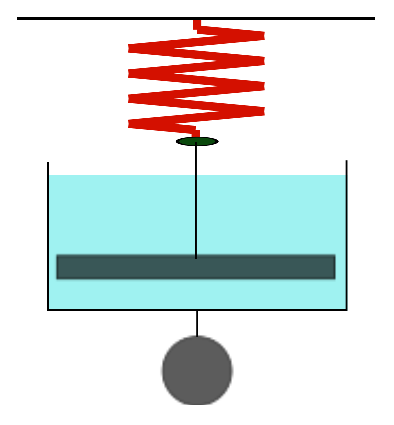
\includegraphics[width = 5cm]{./figures/Maxwell_model_2.eps}
        \caption{マックスウェルモデル}
\end{figure}

\begin{enumerate}
\setlength{\parskip}{0cm} % 段落間
\setlength{\itemsep}{0.5cm} % 項目間

\item
応力 $\sigma (t)$ とひずみ $\gamma(t)$ の関係が以下のように表されることを示せ。
\begin{align*}
G_0 \difd{\gamma (t)}{t}  
	&= \difd{\sigma (t)}{t} + \dfrac{G_0}{\eta} \sigma (t)
%\label{eq:1}
\end{align*}

\begin{itembox}[l]{{\bf ヒント:}}

マックスウェルモデルにおいて、応力はそれぞれの部分に共通となり、歪みはそれぞれの部分の和となることを利用すればよい。

また、バネ部分での釣り合いの式は、Hook の法則 $\sigma = G_0 \gamma$ を用い、ダッシュポット部分では、Newton の法則より、$\sigma = \eta \dot{\gamma}$ となることを用いよ。

\end{itembox}


\item
前問で得た、
\begin{align*}
G_0 \difd{\gamma (t)}{t}  
	&= \difd{\sigma (t)}{t} + \dfrac{G_0}{\eta} \sigma (t)
%\label{eq:1}
\end{align*}
という式を解いて、応力緩和関数 $G(t)$ が以下となることを示せ。
\begin{align*}
G(t) 
	&= G_0 \exp \left(-\dfrac{t}{\tau} \right)
\end{align*}
なお、$\tau$ は、$\tau = \dfrac{\eta}{G_0}$ であり、応力緩和関数が $\dfrac{1}{e}$ となる特徴時間(緩和時間)である。

\begin{itembox}[l]{{\bf ヒント:}}

与えられた微分方程式の右辺を 0 とおけば $\sigma(t)$ についての線形同次方程式となり、容易に解くことができる。
この結果を用いて、積分定数である $C$ を $C \rightarrow C (t)$ として、元の微分方程式に代入して定数変化法で解いていく。

結果的に得た、応力 $\sigma(t)$ についての式を構成方程式と見比べることで、応力緩和関数 $G(t)$ の表式を導出する。

\end{itembox}


\item
このマックスウェルモデルにおいて、貯蔵弾性率 $G'(\omega)$ と損失弾性率 $G''(\omega)$ が以下のように書けることを示せ。
\begin{align*}
\begin{cases}
G' (\omega) = \dfrac{\omega^2 \tau^2}{1+\omega^2 \tau^2} G_0 \\[8pt]
G'' (\omega) = \dfrac{\omega \tau}{1+\omega^2 \tau^2} G_0
\end{cases}
\end{align*}


\begin{itembox}[l]{{\bf ヒント:}}

前問で得た応力緩和関数 $G(t)$ のフーリエ変換を実際に展開した結果を、$i\omega \tilde{G} (\omega) = G'(\omega) + i G''(\omega)$ という関係に代入して、実部と虚部を比較すればよい。

\end{itembox}

\end{enumerate}



\newpage

\begin{enumerate}
\item
応力 $\sigma (t)$ とひずみ $\gamma(t)$ の関係が以下のように表されることを示せ。
\begin{align*}
G_0 \difd{\gamma (t)}{t}  
	&= \difd{\sigma (t)}{t} + \dfrac{G_0}{\eta} \sigma (t)
%\label{eq:1}
\end{align*}

\begin{itembox}[l]{{\bf ヒント:}}

マックスウェルモデルにおいて、応力はそれぞれの部分に共通となり、歪みはそれぞれの部分の和となることを利用すればよい。

また、バネ部分での釣り合いの式は、Hook の法則 $\sigma = G_0 \gamma$ を用い、ダッシュポット部分では、Newton の法則より、$\sigma = \eta \dot{\gamma}$ となることを用いよ。

\end{itembox}

{\bf (解答例)}

系全体でみた場合の歪みと応力を $\gamma, \sigma$ とし、バネの部分に適応されるものを s、ダッシュポットへを d という添え字をつけて分割して考える。

このとき、応力は共通となり、歪みはそれぞれの部分の和となるので、
\begin{equation*}
\begin{cases}
\sigma_s = \sigma_d = \sigma \notag \\
\gamma_s + \gamma_d = \gamma
\end{cases}
\end{equation*}
となる。

バネ部分での釣り合いの式は、バネの剛性率を $G_0$ とすれば、
\begin{align*}
\sigma_s (t) &= G_0 \gamma_s (t) \notag \\
\gamma_s (t) &= \dfrac{1}{G_0} \sigma_s (t) = \dfrac{1}{G_0} \sigma (t) \notag \\
\therefore \quad \dot{\gamma_s} (t) &= \dfrac{1}{G_0} \dot{\sigma} (t)
\end{align*}
なお、一行目の関係は Hook の法則に従った。

一方、ダッシュポット部分の釣り合いは、粘度を $\eta$ として、Newton の法則より、
\begin{align*}
\sigma_d (t) &= \eta \dot{\gamma_d} (t) \notag \\
\therefore \quad \dot{\gamma_d} (t) &= \dfrac{1}{\eta} \sigma_d (t) = \dfrac{1}{\eta} \sigma (t)
\end{align*}

系の歪みがそれぞれの部分の和であるので、
\begin{align*}
\dot{\gamma} (t) 
	&= \dot{\gamma_s} (t) + \dot{\gamma_d} (t) \notag \\ 
	&= \dfrac{1}{G_0} \dot{\sigma} (t) + \dfrac{1}{\eta} \sigma (t)
\end{align*}

時間微分を明示的に書き、
\begin{align*}
G_0 \difd{\gamma (t)}{t}  
	&= \difd{\sigma (t)}{t} + \dfrac{G_0}{\eta} \sigma (t)
%\label{eq:1}
\end{align*}

\vspace{10pt}

\newpage

\item
前問で得た、
\begin{align*}
G_0 \difd{\gamma (t)}{t}  
	&= \difd{\sigma (t)}{t} + \dfrac{G_0}{\eta} \sigma (t)
%\label{eq:1}
\end{align*}
という式を解いて、応力緩和関数 $G(t)$ が以下となることを示せ。
\begin{align*}
G(t) 
	&= G_0 \exp \left(-\dfrac{t}{\tau} \right)
\end{align*}
なお、$\tau$ は、$\tau = \dfrac{\eta}{G_0}$ であり、応力緩和関数が $\dfrac{1}{e}$ となる特徴時間(緩和時間)である。

\begin{itembox}[l]{{\bf ヒント:}}

与えられた微分方程式の右辺を 0 とおけば $\sigma(t)$ についての線形同次方程式となり、容易に解くことができる。
この結果を用いて、積分定数である $C$ を $C \rightarrow C (t)$ として、元の微分方程式に代入して定数変化法で解いていく。

結果的に得た、応力 $\sigma(t)$ についての式を構成方程式と見比べることで、応力緩和関数 $G(t)$ の表式を導出する。

\end{itembox}

{\bf (解答例)}

まず、設問で与えられた微分方程式の右辺を 0 とおいた方程式は、$\sigma(t)$ についての線形同次方程式となり、
\begin{align*}
\difd{\sigma (t)}{t} + \dfrac{G_0}{\eta} \sigma (t) &= 0 \notag \\
\difd{\sigma (t)}{t} &= -\dfrac{G_0}{\eta} \sigma (t) \notag \\
\int \dfrac{1}{\sigma (t)} \diff \sigma (t) &= -\dfrac{G_0}{\eta} \int \diff t \notag \\
\ln \sigma (t) &= -\dfrac{G_0}{\eta} t + C_0 \notag \\
\therefore \quad \sigma(t) &= C \exp \left(-\dfrac{G_0}{\eta} t \right)
%\label{eq:2}
\end{align*}

この結果を用いて、$C \rightarrow C (t)$ として、定数変化法で解いていく。

$\sigma(t)$ を再度、微分方程式に代入すると、以下のように展開できる。
\begin{align*}
G_0 \difd{\gamma (t)}{t}  
	&= \difd{\left[ C(t) \exp \left(-\dfrac{G_0}{\eta} t \right) \right] }{t} + \dfrac{G_0}{\eta} \left[ C(t) \exp \left(-\dfrac{G_0}{\eta} t \right) \right] \\[10pt]
	&= \difd{C(t)}{t}\exp \left(-\dfrac{G_0}{\eta} t \right) -\dfrac{G_0}{\eta} C(t) \exp \left(-\dfrac{G_0}{\eta} t \right) + \dfrac{G_0}{\eta} C(t) \exp \left(-\dfrac{G_0}{\eta} t \right) \\
\therefore \quad \difd{C(t)}{t} & = G_0 \difd{\gamma (t)}{t} \exp \left(\dfrac{G_0}{\eta} t \right) \\
\end{align*}

上式を、$t=0 \sim t$ において積分して以下を得る。
\begin{align*}
\quad C(t) - C_0 = \int_0^t G_0 \difd{\gamma (t')}{t'} 
	\exp \left(\dfrac{G_0}{\eta} t' \right) \diff t'
\end{align*}
なお、$C_0 = C(t=0)$ とした。

この結果を、応力 $\sigma(t)$ についての式に代入して、応力の時間変化 $\sigma(t) $ に関して、以下の表式を得る。
\begin{align*}
\sigma(t) 
	&= \left[\int_0^t G_0 \difd{\gamma (t')}{t'} \exp \left(\dfrac{G_0}{\eta} t' \right) \diff t' + C_0 \right] \exp \left(- \dfrac{G_0}{\eta} t \right) \notag \\
%
	&= \int_0^t \difd{\gamma (t')}{t'} 
		G_0 \exp \left[ -\dfrac{G_0}{\eta} (t-t') \right] \diff t' 
		+ C_0 \exp \left(- \dfrac{G_0}{\eta} t \right)
\end{align*}

対象となる線形粘弾性体の構成方程式は以下であったので、
\begin{equation*}
\sigma(t)=\int_{-\infty}^{t} G(t - t')\dot{\gamma}(t') \diff t'
\end{equation*}

上記の結果と見比べると、
\begin{align}
\begin{cases}
G(t) = G_0 \exp \left[ -\dfrac{G_0}{\eta} t \right] \\
C_0 = 0
\end{cases}
\end{align}

したがって、緩和時間 $\tau$ を $\tau = \dfrac{\eta}{G_0}$ とおいて、以下となる。
\begin{align*}
G(t) 
	&= G_0 \exp \left(-\dfrac{t}{\tau} \right)
\end{align*}

%また、$\sigma(0) = G_0 \gamma_0$ より、
%\begin{align*}
%\sigma(0) 
%	&= G_0 \gamma_0 = (G_0 + C_1) \exp \left(0 \right)\notag \\
%\therefore \quad C_1 &= G_0 (\gamma -1)
%\end{align*}
%


%ここで、設問の条件より、$\sigma(t) = G(t) \gamma_0 $ であったので、結局、
%\begin{align*}
%G(t) 
%	&= \dfrac{1}{\gamma_0} G_0 \gamma_0 \exp \left(-\dfrac{G_0}{\eta} t \right) \notag \\
%	&= G_0 \exp \left(-\dfrac{t}{\tau} \right)
%\end{align*}
%なお、緩和弾性率が $\dfrac{1}{e}$ となる緩和時間として、$\tau = \dfrac{\eta}{G_0}$ とした。

\color{black}

\newpage

\item
このマックスウェルモデルにおいて、貯蔵弾性率 $G'(\omega)$ と損失弾性率 $G''(\omega)$ が以下のように書けることを示せ。
\begin{align*}
\begin{cases}
G' (\omega) = \dfrac{\omega^2 \tau^2}{1+\omega^2 \tau^2} G_0 \\[8pt]
G'' (\omega) = \dfrac{\omega \tau}{1+\omega^2 \tau^2} G_0
\end{cases}
\end{align*}


\begin{itembox}[l]{{\bf ヒント:}}

前問で得た応力緩和関数 $G(t)$ のフーリエ変換を実際に展開した結果を、$i\omega \tilde{G} (\omega) = G'(\omega) + i G''(\omega)$ という関係に代入して、実部と虚部を比較すればよい。

\end{itembox}


{\bf (解答例)}



前問で得た応力緩和関数 $G(t)$ のフーリエ変換を取ると、
\begin{align*}
\tilde{G}(\omega) 
	&= \int_0^{\infty} G(t) e^{-i\omega t } \diff t \notag \\
	&= G_0 \int_0^{\infty} e^{-\left(\dfrac{1}{\tau} + i\omega \right)t} \diff t \notag \\
	&= G_0 \left[ \dfrac{1}{\dfrac{1}{\tau} + i\omega} e^{ -\left(\dfrac{1}{\tau} + i\omega \right)t} \right]_0^{\infty} \notag \\
	&= G_0 \dfrac{1}{\dfrac{1}{\tau} + i\omega} \\
	&= G_0 \dfrac{\tau}{1 + i \omega \tau}
\end{align*}

ここで、前問の解答で示したように、$i\omega \tilde{G} (\omega) = G'(\omega) + i G''(\omega)$ であったので、上式の結果を代入すると、
\begin{align*}
G'(\omega) + i G''(\omega)
	&= G_0 \dfrac{i \omega \tau}{1 + i \omega \tau} \\
	&= G_0 \dfrac{i \omega \tau \left(1 - i \omega \tau \right)}{\left(1 + i \omega \tau \right) \left(1 - i \omega \tau \right)} \\
	&= G_0 \dfrac{\omega^2 \tau^2}{1+ \omega^2 \tau^2} +i G_0 \dfrac{\omega \tau}{1+ \omega^2 \tau^2}
\end{align*}

したがって、
\begin{align*}
\begin{cases}
G' (\omega) = \dfrac{\omega^2 \tau^2}{1+\omega^2 \tau^2} G_0 \\[8pt]
G'' (\omega) = \dfrac{\omega \tau}{1+\omega^2 \tau^2} G_0
\end{cases}
\end{align*}
を得る。

\end{enumerate}

\section{その他の事項}

\subsection{方程式の無次元化}

\begin{boxnote}
現象の基礎方程式が与えられたときに、その方程式で記述される現象を整理するためには、方程式のパラメタの組み合わせから構成される「無次元パラメタ」を使用することが重要です。
本問では、基礎方程式に「変数の無次元化」を施すことにより、この無次元パラメタを導き出す方法を確認します。

%まず、物質の移動を表現する「拡散方程式」について、無次元化を行う。
%さらに、高分子流体などの流体力学を説くときの基本方程式である Navier-Stokes(NS) 方程式に無次元化を適用することで、NS 流体を特徴付ける無次元パラメタである「レイノルズ数」を導いてみます。

\end{boxnote}

\vspace{10pt}

\begin{enumerate}
\setlength{\parskip}{0cm} % 段落間
\setlength{\itemsep}{0.5cm} % 項目間
\item
拡散方程式

以下の表式で表される、拡散方程式
\begin{equation*}
\difp{f(x, t)}{t} = D \difpp{f(x, t)}{x}
\end{equation*}
に対して、長さと時間の単位量(${\it l}_0$、$t_0$ )と無次元量($\tilde{x}$ および $\tilde{t}$)を用いて、次のような変数変換(無次元化)を行う。
\begin{equation*}
\begin{cases}
x= {\it l}_0 \tilde{x} \\
t = t_0 \tilde{t}
\end{cases}
\end{equation*}
%ここに、${\it l}_0$ と $t_0$ は長さと時間の単位量であり、$\tilde{x}$ と $\tilde{t}$ は無次元量である。
単位量 ${\it l}_0$ と $t_0$ を適切に選ぶことにより、上の拡散方程式は常に次の基本形に変換できることを示せ。
\begin{equation*}
\difp{\tilde{f}(\tilde{x}, \tilde{t})}{\tilde{t}} = \difpp{ \tilde{f}(\tilde{x}, \tilde{t})}{\tilde{x}}
\end{equation*}

\begin{itembox}[l]{{\bf ヒント:}}
単位量と無次元量に関する適切な関係式を元の拡散方程式に代入して数係数をまとめたうえで、この項を都合の良い値(一般には、1 とする場合が多い)となるように設定すればよい。

なお、この基本形の性質を求めることで、任意の係数(拡散係数の値など)の場合について、その性質を理解できたことになる。

\end{itembox}


\item
Navier-Stokes 方程式

非圧縮流体の運動を記述する Navier-Stokes 方程式は以下のように表される。
\begin{equation*}
\rho\dfrac{\partial \bm{v}}{\partial t} + \rho \bm{v} \cdot \nabla \bm{v} = - \nabla P + \eta \Delta \bm{v} + \bm{K}
\end{equation*}
ここに、$\rho$ は流体の密度(非圧縮のため一定と仮定)、$\bm{v}$ は流体の流速、$P$ は局所的な圧力、$\eta$ は粘性係数(一定と仮定)、$\bm{K}$ はこの流体に作用する外力(重力など)である。

この式に対して先の問題と同じように無次元化を行うと、(外力の項は別として)単位をうまく選んでも消せないパラメタが残る。
このようなパラメタがレイノルズ数
\begin{equation*}
Re = \dfrac{\rho \left(\dfrac{{\it l}_0^2}{t_0} \right)}{\eta}
\end{equation*}
であることを示せ。

\begin{itembox}[l]{{\bf ヒント:}}
無次元化するための単位量として、長さ $l_0$、時間 $t_0$、質量 $m_0$ を設定して、圧力については、 
$P = \dfrac{m_0}{l_0 (t_0)^2} \tilde{P}$ と換算して考えればよい。

なお、この結果は、粘性流体の性質はレイノルズ数を決めれば決まってしまうことを表していることになる。

\end{itembox}


\item 経路積分の無次元化 

SCF 理論において、経路積分 $Q(s, \bm{r}: s', \bm{r'})$ は以下の式で表され、ポリマー鎖のコンフォメーションを考慮した形で平衡状態における鎖中のセグメントの濃度分布を求めることが出来る。 
\begin{equation*}
\difp{Q(s, \bm{r}: s', \bm{r'})}{s} = \dfrac{b^2}{6} \nabla^2 Q(s, \bm{r}: s', \bm{r'}) - V(\bm{r}) Q(s, \bm{r}: s', \bm{r'})
\end{equation*}
ここで、$s, s'$ はポリマー鎖中のセグメントを指定するインデックス、$\bm{r}, \bm{r'}$ は位置ベクトル、$V(\bm{r})$ は自己無撞着場であり、$b$ は有効結合帳である。

$s$ と $\bm{r}$ に対して以下のように単位量を定めて無次元化し、物理的に意味を持つ無次元パラメタを見出せ。

\begin{align*}
\begin{cases}
s= s_0 \tilde{s} \\
\bm{r} = l_0 \tilde{\bm{r}}
\end{cases}
\end{align*}

\begin{itembox}[l]{{\bf ヒント:}}

上記の無次元化により、数係数 $\dfrac{s_0 b^2}{6} \dfrac{1}{l_0^2} $ を得る。
数係数の処理にはいろいろな考え方を適応することが可能であるが、例えば、
$s_0$ にポリマーの鎖長を表すセグメント数 $N$ を当てはめて、数係数が 1 となるようにおけば、以下のようになり、単位長さをポリマーの慣性半径となるように定めることになる。
\begin{align*}
l_0 = \sqrt{\dfrac{N b^2}{6}} = R_g
\end{align*}

\end{itembox}

\end{enumerate}

\newpage


\begin{enumerate}
\setlength{\parskip}{0cm} % 段落間
\setlength{\itemsep}{0.5cm} % 項目間

\item
拡散方程式

以下の表式で表される、拡散方程式
\begin{equation*}
\difp{f(x, t)}{t} = D \difpp{f(x, t)}{x}
\end{equation*}
に対して、長さと時間の単位量(${\it l}_0$、$t_0$ )と無次元量($\tilde{x}$ および $\tilde{t}$)を用いて、次のような変数変換(無次元化)を行う。
\begin{equation*}
\begin{cases}
x= {\it l}_0 \tilde{x} \\
t = t_0 \tilde{t}
\end{cases}
\end{equation*}
%ここに、${\it l}_0$ と $t_0$ は長さと時間の単位量であり、$\tilde{x}$ と $\tilde{t}$ は無次元量である。
単位量 ${\it l}_0$ と $t_0$ を適切に選ぶことにより、上の拡散方程式は常に次の基本形に変換できることを示せ。
\begin{equation*}
\difp{\tilde{f}(\tilde{x}, \tilde{t})}{\tilde{t}} = \difpp{ \tilde{f}(\tilde{x}, \tilde{t})}{\tilde{x}}
\end{equation*}

\begin{itembox}[l]{{\bf ヒント:}}
単位量と無次元量に関する適切な関係式を元の拡散方程式に代入して数係数をまとめたうえで、この項を都合の良い値(一般には、1 とする場合が多い)となるように設定すればよい。

なお、この基本形の性質を求めることで、任意の係数(拡散係数の値など)の場合について、その性質を理解できたことになる。

\end{itembox}

\vspace{10pt}

{\bf (解答例)}

関数 $f(x, t)$ が数密度だとすると、
\begin{align*}
\begin{cases}
f(x,t) = \dfrac{1}{(l_0)^3} \tilde{f}(\tilde{x}, \tilde{t}) \notag \\[10pt]
\difp{}{t} = \dfrac{1}{t_0} \difp{}{\tilde{t}} \notag \\[10pt]
\difpp{}{x} = \dfrac{1}{l_0^2} \difpp{}{\tilde{x}}
\end{cases}
\end{align*}

これらの関係式を元の拡散方程式に代入して、数係数をまとめると、
\begin{align*}
&\dfrac{1}{t_0} \difp{}{\tilde{t}} \dfrac{1}{(l_0)^3} \tilde{f}(\tilde{x}, \tilde{t}) = D \dfrac{1}{l_0^2} \difpp{}{\tilde{x}} \dfrac{1}{(l_0)^3} \tilde{f}(\tilde{x}, \tilde{t}) \notag \\
\therefore \quad &\dfrac{1}{D} \dfrac{l_0^2}{t_0} \difp{}{\tilde{t}} \tilde{f}(\tilde{x}, \tilde{t}) = \difpp{}{\tilde{x}} \tilde{f}(\tilde{x}, \tilde{t})
\end{align*}

したがって、$\dfrac{1}{D} \dfrac{l_0^2}{t_0} = 1$ となるように長さ、あるいは、時間の単位を選べば、単位や係数項にとらわれることなく拡散現象を計算できることになる。

具体的には、以下のような関係となるように基準単位を選べばよい。
\begin{align*}
\begin{cases}
t_0 = \dfrac{l_0^2}{D} \\
\text{あるいは} \\
l_0 = \sqrt{D t_0}
\end{cases}
\end{align*}


\newpage

\item
Navier-Stokes 方程式

非圧縮流体の運動を記述する Navier-Stokes 方程式は以下のように表される。
\begin{equation*}
\rho\dfrac{\partial \bm{v}}{\partial t} + \rho \bm{v} \cdot \nabla \bm{v} = - \nabla P + \eta \Delta \bm{v} + \bm{K}
\end{equation*}
ここに、$\rho$ は流体の密度(非圧縮のため一定と仮定)、$\bm{v}$ は流体の流速、$P$ は局所的な圧力、$\eta$ は粘性係数(一定と仮定)、$\bm{K}$ はこの流体に作用する外力(重力など)である。

この式に対して先の問題と同じように無次元化を行うと、(外力の項は別として)単位をうまく選んでも消せないパラメタが残る。
このようなパラメタがレイノルズ数
\begin{equation*}
Re = \dfrac{\rho \left(\dfrac{{\it l}_0^2}{t_0} \right)}{\eta}
\end{equation*}
であることを示せ。

\begin{itembox}[l]{{\bf ヒント:}}
無次元化するための単位量として、長さ $l_0$、時間 $t_0$、質量 $m_0$ を設定して、圧力については、 
$P = \dfrac{m_0}{l_0 (t_0)^2} \tilde{P}$ と換算して考えればよい。

なお、この結果は、粘性流体の性質はレイノルズ数を決めれば決まってしまうことを表していることになる。

\end{itembox}

\vspace{10pt}
{\bf (解答例)}

ここで、無次元化するための単位量(ものさし)として、
\begin{align*}
\begin{cases}
\text{長さ} \quad l_0 \\
\text{時間} \quad t_0 \\
\text{質量} \quad m_0 
\end{cases}
\end{align*}
とすると、
\begin{equation*}
\begin{cases}
%x_i = l_0 \tilde{x_i}  \notag \\[8pt]
%t = t_0 \tilde{t} \notag \\[8pt]
v_i = \dfrac{l_0}{t_0} \tilde{v_i} \notag \\[8pt]
\nabla = \dfrac{1}{l_0} \tilde{\nabla} \notag \\[8pt]
P = \dfrac{m_0}{l_0 (t_0)^2} \tilde{P} \notag \\[8pt]
\Delta = \dfrac{1}{(l_0)^2} \tilde{\Delta}
\end{cases}
\end{equation*}

これらの無次元量を用いて、 Navier-Stokes 方程式(外力の項は無視した)は以下のように展開できる。
\begin{align*}
\rho \dfrac{l_0}{t_0} \dfrac{1}{t_0} \dfrac{\partial \tilde{v}_i}{\partial \tilde{t}} + \rho \dfrac{l_0}{t_0} \tilde{v_i} \cdot \dfrac{1}{l_0} \tilde{\nabla} \dfrac{l_0}{t_0} \tilde{v_i} &= - \dfrac{1}{l_0} \tilde{\nabla} \dfrac{m_0}{l_0 (t_0)^2} \tilde{P} + \eta \dfrac{1}{(l_0)^2} \tilde{\Delta} \dfrac{l_0}{t_0} \tilde{v_i} \notag \\
\dfrac{\rho l_0}{(t_0)^2} \dfrac{\partial \tilde{v}_i}{\partial \tilde{t}} + \dfrac{\rho l_0}{(t_0)^2} \tilde{v_i} \cdot \tilde{\nabla} \tilde{v_i} &= - \dfrac{m_0}{(l_0)^2 (t_0)^2} \tilde{\nabla} \tilde{P} + \dfrac{\eta}{l_0 t_0} \tilde{\Delta} \tilde{v_i} \notag \\
\difp{\tilde{v}_i}{\tilde{t}} + \tilde{v_i} \cdot \tilde{\nabla} \tilde{v_i} &= - \dfrac{(t_0)^2}{\rho l_0} \dfrac{m_0}{(l_0)^2 (t_0)^2} \tilde{\nabla} \tilde{P} + \dfrac{(t_0)^2}{\rho l_0} \dfrac{\eta}{l_0 t_0} \tilde{\Delta} \tilde{v_i} \notag \\
\therefore \quad \difp{\tilde{v}_i}{\tilde{t}} + \tilde{v_i} \cdot \tilde{\nabla} \tilde{v_i} &= - \dfrac{m_0}{\rho (l_0)^3} \tilde{\nabla} \tilde{P} + \dfrac{\eta t_0}{\rho (l_0)^2} \tilde{\Delta} \tilde{v_i}
\end{align*}

したがって、右辺の第一項にまとまった数係数 $\dfrac{m_0}{\rho (l_0)^3} = 1$ となるように、例えば、$m_0  = \rho (l_0)^3$ のように単位量を選定すれば、第二項に、設問中に示された「慣性力と粘性力の比である無次元パラメタのレイノルズ数」の逆数が残ることになる。
\begin{align*}
\difp{\tilde{v}_i}{\tilde{t}} + \tilde{v_i} \cdot \tilde{\nabla} \tilde{v_i} &= - \tilde{\nabla} \tilde{P} + \dfrac{1}{\left( \dfrac{\rho \dfrac{(l_0)^2}{t_0}}{\eta} \right)} \tilde{\Delta} \tilde{v_i}
\end{align*}

\newpage

\item 経路積分の無次元化 

SCF 理論において、経路積分 $Q(s, \bm{r}: s', \bm{r'})$ は以下の式で表され、ポリマー鎖のコンフォメーションを考慮した形で平衡状態における鎖中のセグメントの濃度分布を求めることが出来る。 
\begin{equation*}
\difp{Q(s, \bm{r}: s', \bm{r'})}{s} = \dfrac{b^2}{6} \nabla^2 Q(s, \bm{r}: s', \bm{r'}) - V(\bm{r}) Q(s, \bm{r}: s', \bm{r'})
\end{equation*}
ここで、$s, s'$ はポリマー鎖中のセグメントを指定するインデックス、$\bm{r}, \bm{r'}$ は位置ベクトル、$V(\bm{r})$ は自己無撞着場であり、$b$ は有効結合帳である。

$s$ と $\bm{r}$ に対して以下のように単位量を定めて無次元化し、物理的に意味を持つ無次元パラメタを見出せ。

\begin{align*}
\begin{cases}
s= s_0 \tilde{s} \\
\bm{r} = l_0 \tilde{\bm{r}}
\end{cases}
\end{align*}

\begin{itembox}[l]{{\bf ヒント:}}

上記の無次元化により、数係数 $\dfrac{s_0 b^2}{6} \dfrac{1}{l_0^2} $ を得る。
数係数の処理にはいろいろな考え方を適応することが可能であるが、例えば、
$s_0$ にポリマーの鎖長を表すセグメント数 $N$ を当てはめて、数係数が 1 となるようにおけば、以下のようになり、単位長さをポリマーの慣性半径となるように定めることになる。
\begin{align*}
l_0 = \sqrt{\dfrac{N b^2}{6}} = R_g
\end{align*}

\end{itembox}

\vspace{10pt}
{\bf (解答例)}

設問中の単位量を用いて無次元化すると、
\begin{align*}
\dfrac{1}{s_0} \difp{\tilde{Q}(\tilde{s}, \tilde{\bm{r}}: \tilde{s}', \tilde{\bm{r}}')}{\tilde{s}} &= \dfrac{b^2}{6} \dfrac{1}{l_0^2} \tilde{\nabla}^2 \tilde{Q}(\tilde{s}, \tilde{\bm{r}}: \tilde{s}', \tilde{\bm{r}}') - V(\bm{r}) \tilde{Q}(\tilde{s}, \tilde{\bm{r}}: \tilde{s}', \tilde{\bm{r}}') \\
\therefore \quad \difp{\tilde{Q}(\tilde{s}, \tilde{\bm{r}}: \tilde{s}', \tilde{\bm{r}}')}{\tilde{s}} &= \dfrac{s_0 b^2}{6} \dfrac{1}{l_0^2} \tilde{\nabla}^2 \tilde{Q}(\tilde{s}, \tilde{\bm{r}}: \tilde{s}', \tilde{\bm{r}}') - s_0 V(\bm{r}) \tilde{Q}(\tilde{s}, \tilde{\bm{r}}: \tilde{s}', \tilde{\bm{r}}')
\end{align*}

また、自己無撞着場は位置 $\bm{r}$ において $K$ 種のセグメントが平均場から受ける相互作用を表すので $\displaystyle V(\bm{r}) = \sum_{K'} \chi_{K K'} \phi_{K'}$ であるから $\chi \tilde{\phi}$ と書くと、結局、与式は以下のように変形できる。
\begin{align*}
\difp{\tilde{Q}(\tilde{s}, \tilde{\bm{r}}: \tilde{s}', \tilde{\bm{r}}')}{\tilde{s}} = \dfrac{s_0 b^2}{6} \dfrac{1}{l_0^2} \tilde{\nabla}^2 \tilde{Q}(\tilde{s}, \tilde{\bm{r}}: \tilde{s}', \tilde{\bm{r}}') - s_0 \chi \tilde{\phi} \tilde{Q}(\tilde{s}, \tilde{\bm{r}}: \tilde{s}', \tilde{\bm{r}}')
\end{align*}

ここで、右辺第一項にまとめた数係数 $\dfrac{s_0 b^2}{6} \dfrac{1}{l_0^2} $ に注目しよう。
$s_0$ にポリマーの鎖長を表すセグメント数 $N$ を当てはめて、数係数が 1 となるようにおけば、結局、
\begin{align*}
l_0 = \sqrt{\dfrac{N b^2}{6}} = R_g
\end{align*}
単位長さをポリマーの慣性半径となるように定めることになる。

このとき、
\begin{align*}
\difp{\tilde{Q}(\tilde{s}, \tilde{\bm{r}}: \tilde{s}', \tilde{\bm{r}}')}{\tilde{s}} = \tilde{\nabla}^2 \tilde{Q}(\tilde{s}, \tilde{\bm{r}}: \tilde{s}', \tilde{\bm{r}}') - N \chi \tilde{\phi} \tilde{Q}(\tilde{s}, \tilde{\bm{r}}: \tilde{s}', \tilde{\bm{r}}')
\end{align*}
と書くことが出来ることになり、ポリマーの慣性半径 $R_g$ を長さの単位として、$\chi N$ という無次元パラメタで系を記述できることになる。 


\color{black}

\end{enumerate}



\end{document}